\newcommand*{\ATLASLATEXPATH}{latex/}

\documentclass[UKenglish,texlive=2013]{\ATLASLATEXPATH atlasdoc}

% The language of the document must be set: usually UKenglish or USenglish.

% british and american also work!
% Commonly used options:
%  texlive=YYYY          Specify TeX Live version (2013 is default).
%  atlasstyle=true|false Use ATLAS style for document (default).
%  coverpage             Create ATLAS draft cover page for collaboration circulation.
%                        See atlas-draft-cover.tex for a list of variables that should be defined.
%  cernpreprint          Create front page for a CERN preprint.
%                        See atlas-preprint-cover.tex for a list of variables that should be defined.
%  PAPER                 The document is an ATLAS paper (draft).
%  CONF                  The document is a CONF note (draft).
%  PUB                   The document is a PUB note (draft).
%  txfonts=true|false    Use txfonts rather than the default newtx - needed for arXiv submission.
%  paper=a4|letter       Set paper size to A4 (default) or letter.

\usepackage{\ATLASLATEXPATH atlaspackage}
\usepackage{\ATLASLATEXPATH atlasbiblatex}
\usepackage{\ATLASLATEXPATH atlascontribute}
\usepackage{\ATLASLATEXPATH atlasphysics}

\usepackage{tabulary}

\addbibresource{muonrawhits.bib}
\addbibresource{bibtex/bib/ATLAS.bib}

\graphicspath{{logos/}{figures/}}

\usepackage{muonrawhits-defs}

\AtlasTitle{Studies of the ATLAS MDT and CSC hit rates using proton-proton collisions at 13 TeV}

\author{The ATLAS Collaboration}

\AtlasVersion{0.1}

\AtlasRefCode{MUON-2015-XXX}

% \AtlasNote{ATL-COM-PHYS-2014-XXX}

\AtlasAbstract{%
  This is a bare bones ATLAS document. Put the abstract for the document here.
}

% The following information is needed for the cover page. The commands are only defined
% if you use the coverpage option in atlasdoc or use the atlascover package

% \AtlasCoverSupportingNote{Short title note 1}{https://cds.cern.ch/record/XXXXXXX}
% \AtlasCoverSupportingNote{Short title note 2}{https://cds.cern.ch/record/YYYYYYY}

% Comment deadline
% \AtlasCoverCommentsDeadline{DD Month 2014}

% Analysis team members - contact editors should no longer be specified
% as there is a generic email list name for the editors
% \AtlasCoverAnalysisTeam{Peter Analyser, Susan Editor1, Jenny Editor2, Alphonse Physicien}

% A PUB note has readers and not an EdBoard -- give their names here (one line or several entries)
% \AtlasCoverReaderMember{Reader~1, Reader~2}
% \AtlasCoverReaderMember{Reader~1}
% \AtlasCoverEdBoardMember{Reader~2}




\hypersetup{pdftitle={ATLAS draft},pdfauthor={The ATLAS Collaboration}}

\begin{document}

\maketitle

\tableofcontents

% List of contributors - print here or after the Bibliography.
%\PrintAtlasContribute{0.30}
%\clearpage

\section{Introduction}
\label{sec:intro}

Muons are important at $\pt$ of a few GeV ($H\rightarrow ZZ^\star\rightarrow 4\ell$, $H\rightarrow J/\psi \gamma \rightarrow 2\ell\gamma$) and up to $\pt$ of many TeV ($W'$, $Z'$).

The MDTs had problems in 2012 and were upgraded during LS1 to address this. The CSCs had updates to the RODs during LS1. Understanding their performance in new data is important.

In the next long shutdown, projected to be in 2018, the current small wheel will be replaced by the so-called New Small Wheel (NSW). One of the driving performance requirements of the NSW is the ability to cope with a large flux of incident particles. Extrapolating the current particle flux to post-LS2 conditions is therefore important.

Section \ref{sec:detector} describes the ATLAS detector, and in particular, the MDTs and CSCs. Section \ref{sec:dataset} describes the data set used in this study. Section \ref{sec:hitrates} describes the measured hit rates in the MDTs and CSCs as a function of detector region, luminosity, distance from the beam pipe. Section \ref{sec:extrapolations} describes extrapolations of the hit rates from the current LHC conditions to Run 3 and the HL-LHC conditions. Section \ref{sec:conclusions} concludes with a summary of the studies.



\section{The ATLAS detector}
\label{sec:detector}

The ATLAS detector is a multi-purpose detector at the Large Hadron Collider (LHC). It is a nearly hermetic detector built to measure the trajectory and momenta of particles arising from proton-proton collisions. 

The Inner Detector (ID) measures the trajectory of charged particles immersed in a multi-tesla solenoidal magnetic field, thus providing precise momentum measurements. It is composed of three detector technologies: silicon pixels, silicon strips (SCT), and a transition radiation tracker (TRT). It is surrounded by non-compensating electromagnetic and hadronic calorimeters, whose active material are liquid argon and scintillator, respectively.

Outside the ID and calorimeters, the muon spectrometer (MS) exists to measure the trajectory of muons immersed in a multi-tesla toroidal magnetic field. The MS consists of three concentric shells, or ``layers'', split into barrel and endcap regions. Four detector technologies are used: monitored drift tubes (MDTs) and cathode strip chambers (CSCs) provide precise momentum measurements, and resistive plate chambers (RPCs) and thin gap chambers (TGCs) provide fast measurements for triggering at the 40 MHz LHC collision rate. The MDTs and the CSCs are the focus of this note.

The MDTs consist of $\sim\!400,000$ drift tubes and cover the most of the MS. They are used up to $|\eta| < 2.7$ in the middle and outer layers, and up to $|\eta| < 2.0$ in the inner layer, where the incident particle flux becomes unmanageable. The tubes are grouped into chambers which consist of three to eight layers of drift tubes. The gas mixture in the tubes is 93\% Ar and 7\% $\text{CO}_2$, which have a maximal drift time of about $\sim\!700$ ns.

The CSCs are deployed in the region $2.0 < |\eta| < 2.7$ of the endcap inner layer, which is the region closest to the beampipe and subject to the largest incident particle flux. The CSCs are multiwire proportional chambers with cathode planes segmented into strips in orthogonal directions for measurements of $\eta$ and $\phi$. In this study, only the $\eta$ strips are considered in the measurement of hit rates because they are finer than the $\phi$ strips and offer information about the dependence of the hit rate on the distance from the beampipe. Neighboring hit strips are grouped into clusters, and the spatial coordinates are derived from a charge-dependent interpolation of this cluster.

Some naming conventions are adopted in this note. The MS is divided in the $\phi$-plane into 16 sectors, 8 of which are referred to as ``large'' (L) sectors and 8 of which are ``small'' (S), determined by their coverage in $\phi$. The three concentric layers are referred to as the Inner, Middle, and Outer layers according to the distance from the interaction point. Within a layer, the chambers are further divided into $\eta$ stations between 1 and 8, also according to their distance from the IP. Last, the positive (negative) $z$ region of the MS is referred to as the A (C) side.

Groups of chambers are designated with acronyms of this information -- for example, the MDT EIL1 chambers refer to the large sectors of the first $\eta$ station of MDT chambers in the inner endcap, including all $\phi$ sectors. In this note, the hit rates are not divided into $\phi$ sectors since the hit rates are generally symmetric in this coordinate. These conventions are shown schematically in Figure~\ref{fig:detector-ms}.

\begin{figure}
  \begin{center}
    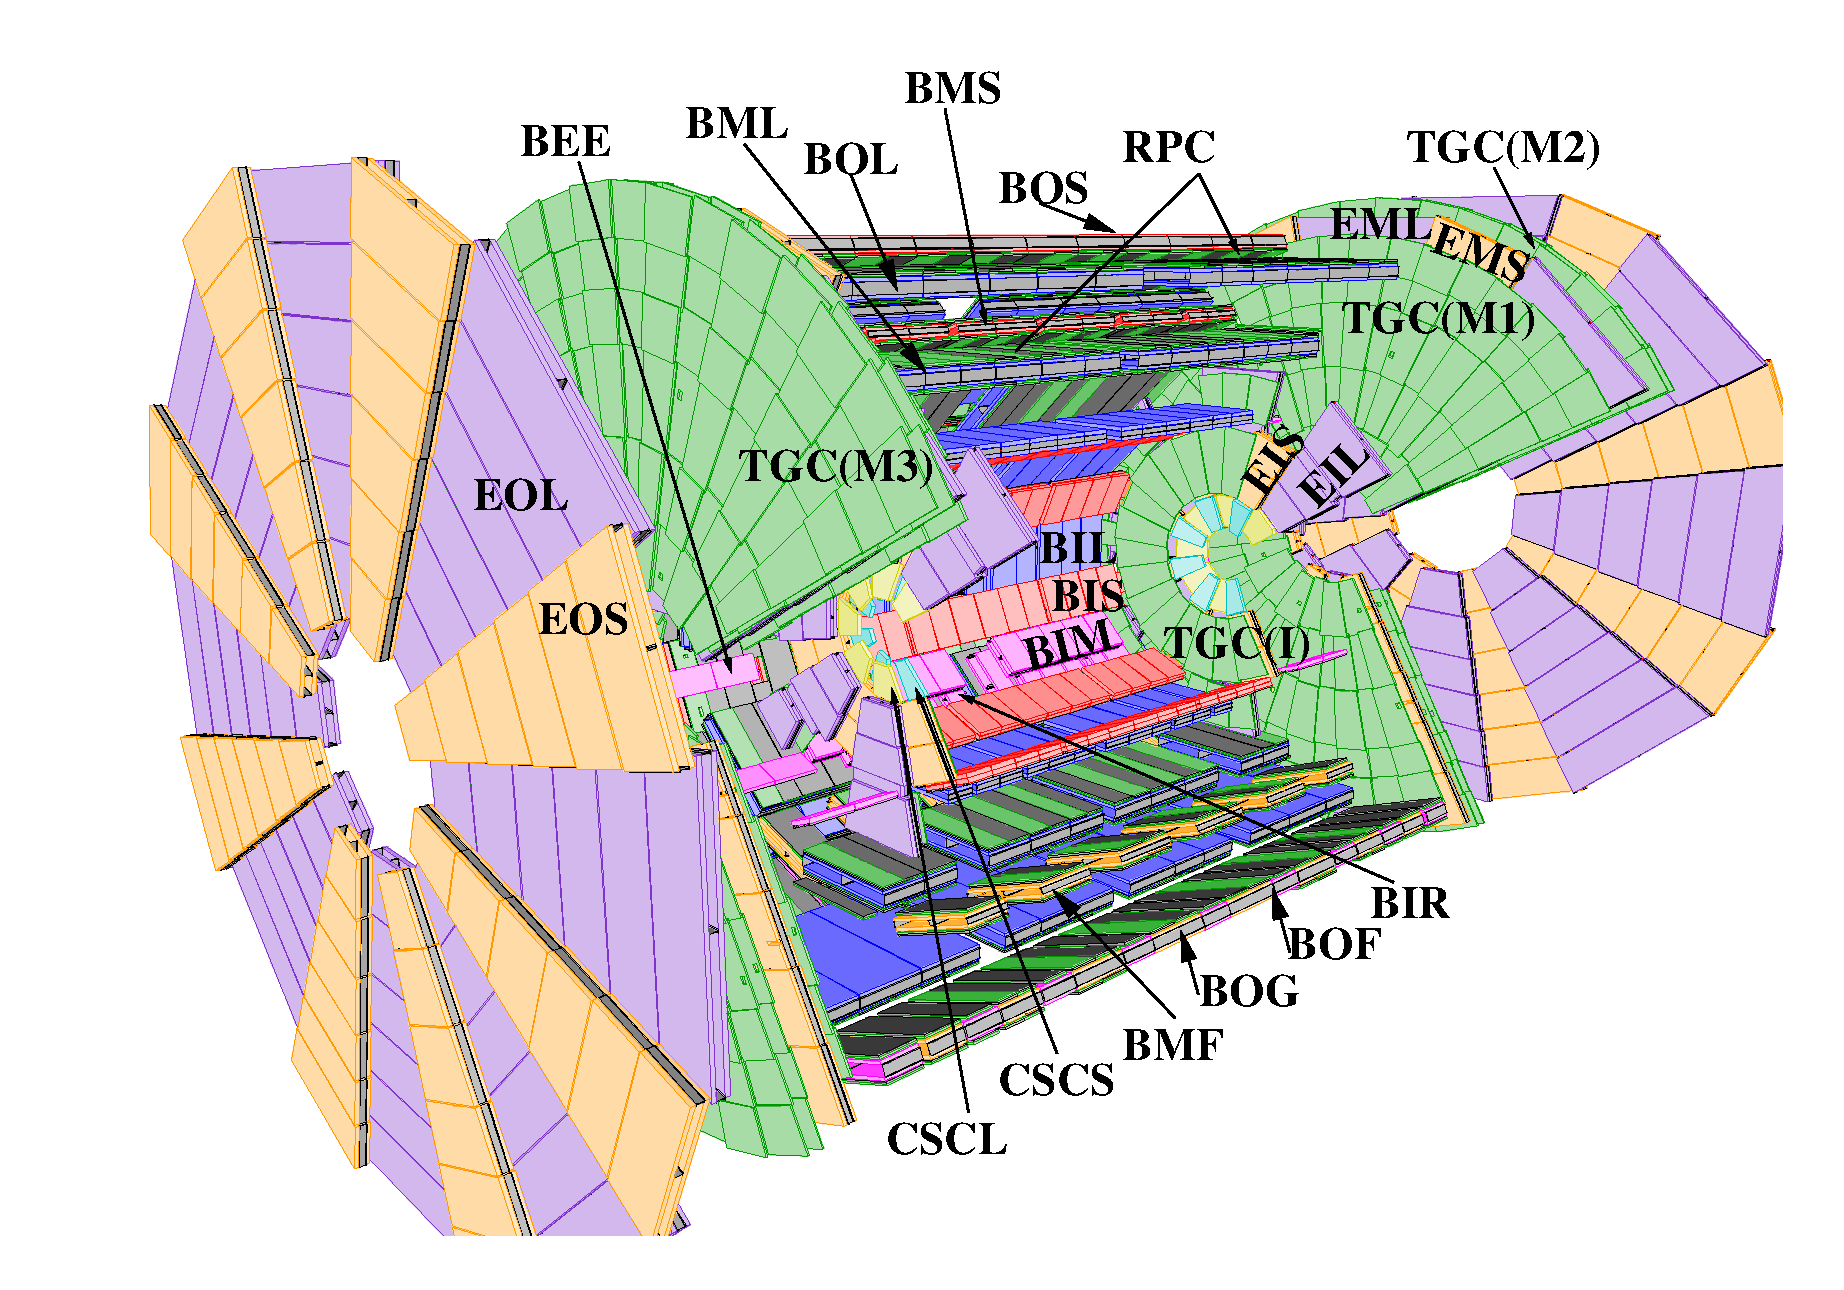
\includegraphics[width=0.80\textwidth]{./figures/TDR_Muon_system_Initial.pdf}
    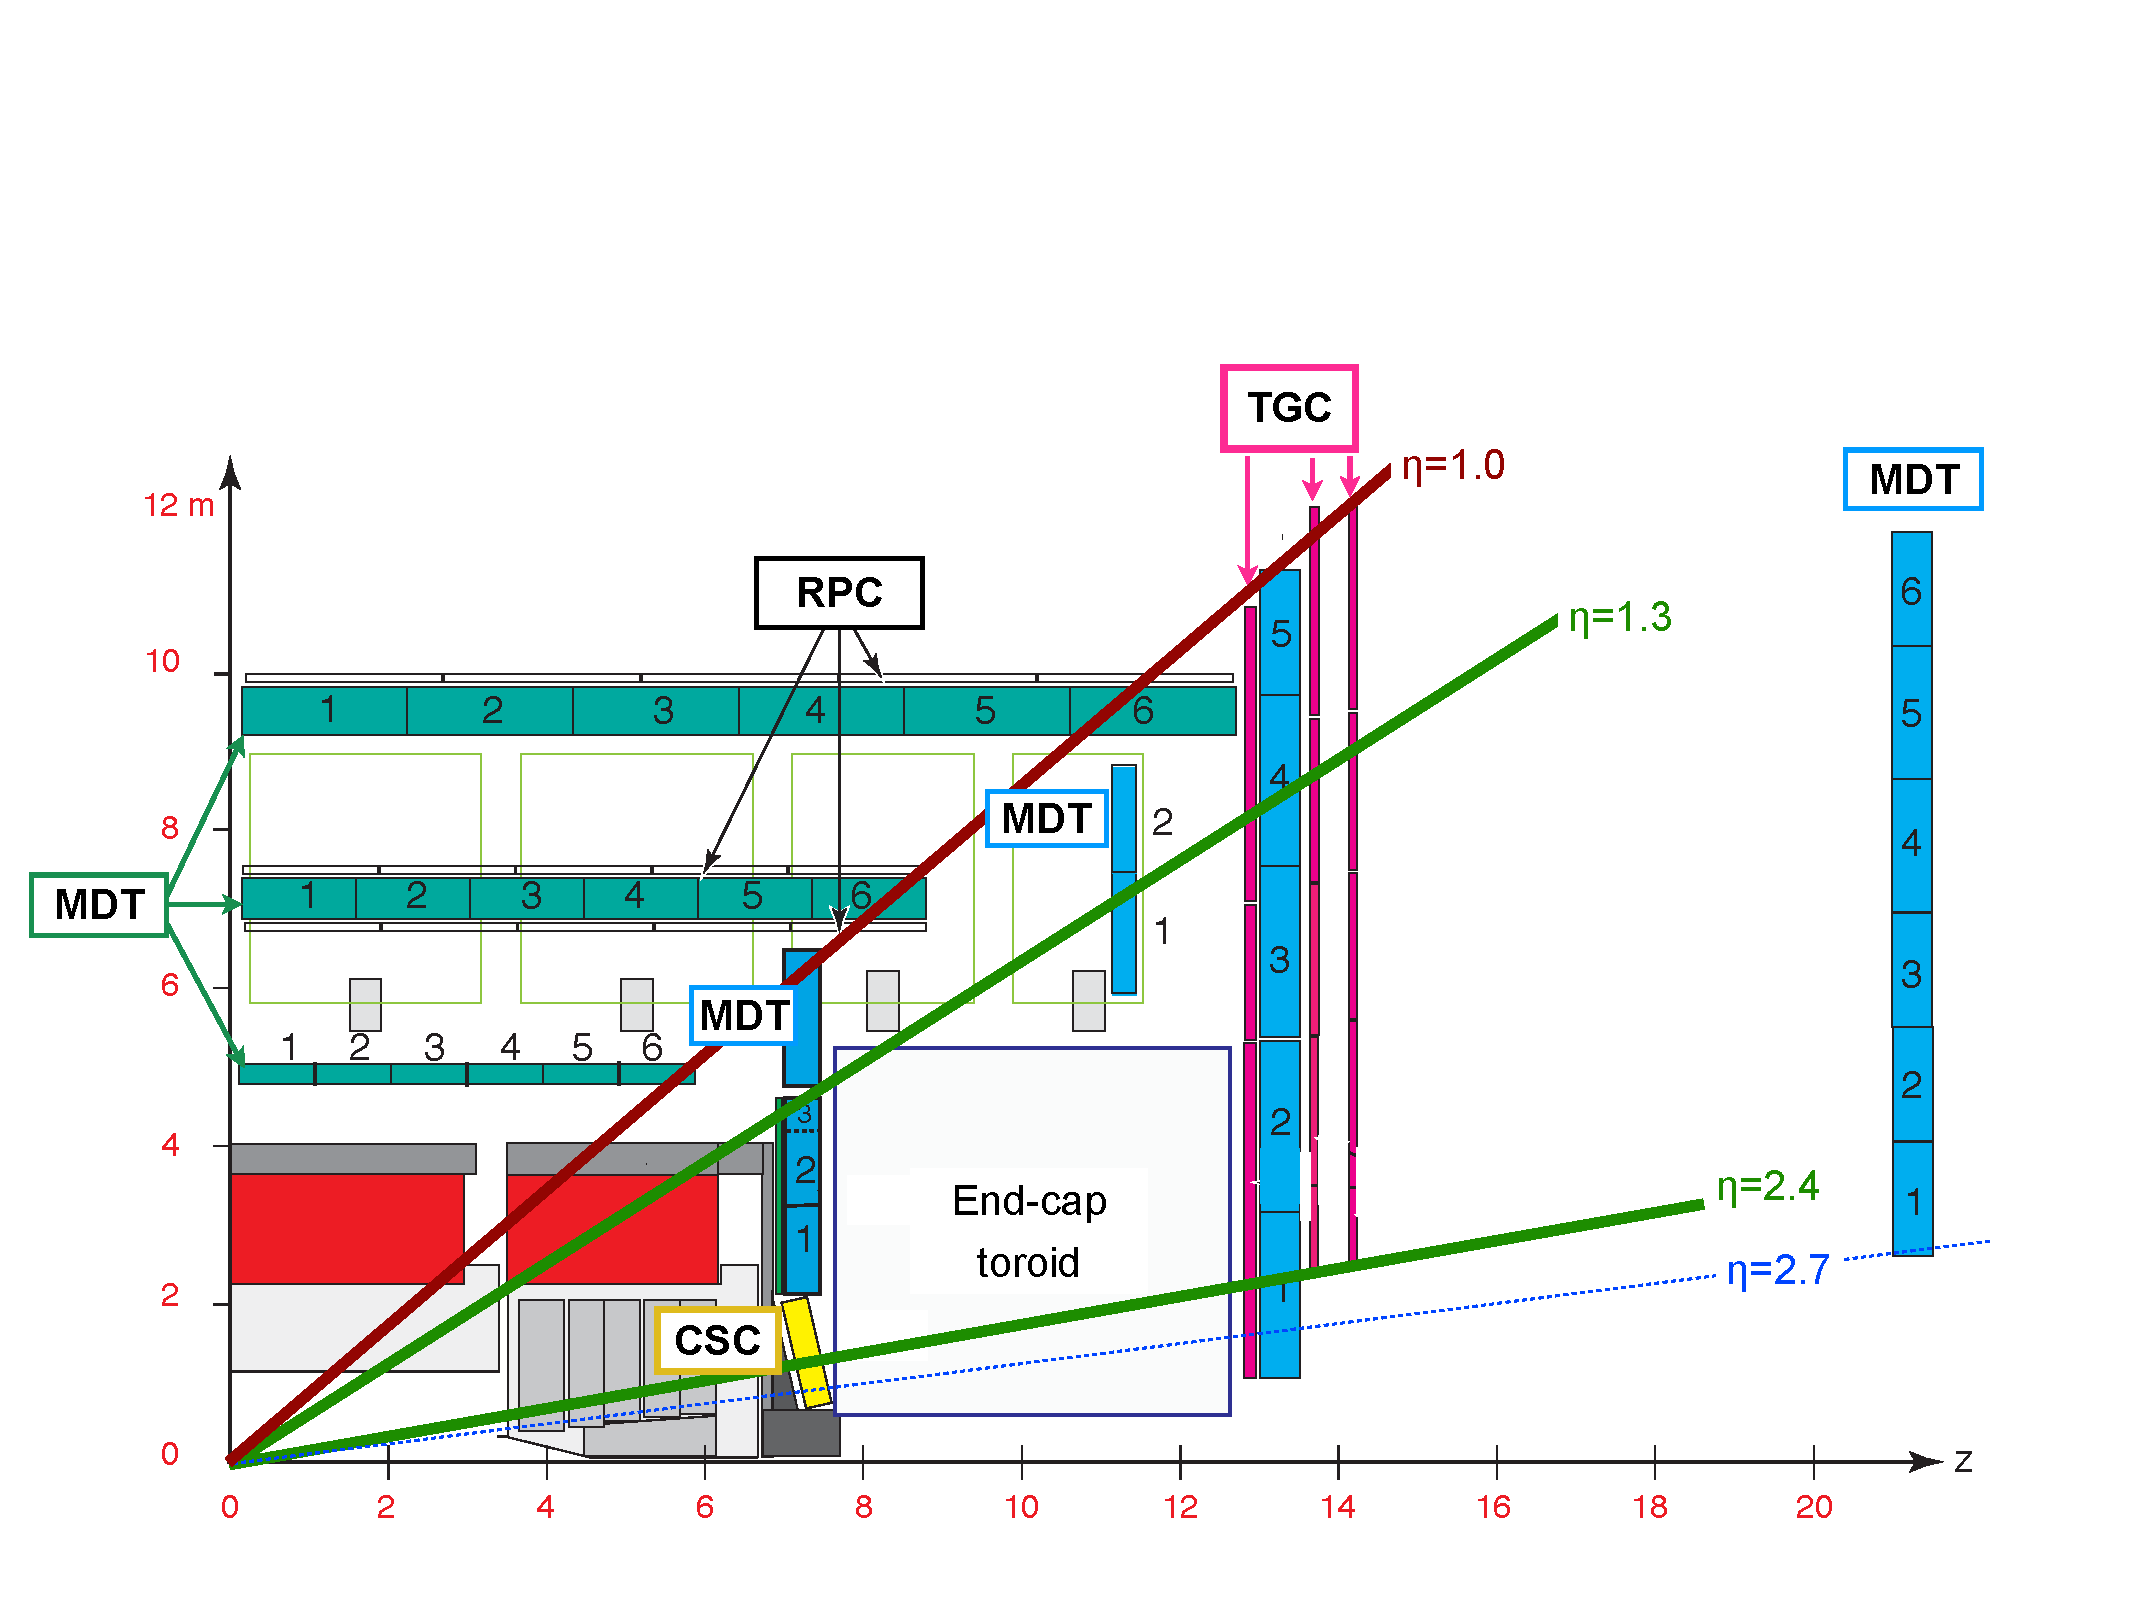
\includegraphics[width=0.80\textwidth]{./figures/TRIG-2012-03_fig_01.pdf}
    \caption{Schematic pictures from the TDR showing a cross-section (top) and quarter-section (bottom) of the muon system. The MDT chambers in the barrel are arranged in three concentric cylindrical shells around the beam axis. In the endcap region, muon chambers form large wheels, perpendicular to the z-axis. In the forward region, CSC is used in the innermost tracking layer. The RPC and TGC chambers are arranged in three layers (called stations) as indicated in the figure.}
    \label{fig:detector-ms}
  \end{center}
\end{figure}



\section{Data set}
\label{sec:data}

The data in this note are taken from proton-proton collisions provided by the LHC in 2015. The collision energy increased from 8 TeV to 13 TeV and the spacing of proton bunches decreased from 50 ns to 25 ns. 

The bunch structure of the LHC proton beams changed throughout 2015 as the machine was commissioned. The MDTs are especially sensitive to this structure because they have a long livetime of 1300 ns (52 BC) and are therefore susceptible to particle fluxes before and after the collision of interest. For comparison, the TGCs have a livetime of 50 ns.

Data are only included if all ATLAS detectors and magnets are operational and fit for physics analysis.

To study a generic sample of proton-proton collisions, events are selected if they pass a so-called ``zero bias'' trigger. The zero bias trigger fires one LHC orbit after a EM15 trigger fires, thus providing an unbiased and luminosity-dependent sample of collisions. The trigger is prescaled to have a rate of 5 Hz. 



\section{Hit rates}
\label{sec:hitrates}

The majority of hits in the MDTs and CSCs are due to \textit{cavern background}, not muons. Cavern background is a mixture of prompt particles from a recent proton collisions and long-lived particles accumulated from many collisions before and after the collision of interest. The most abundant particles in the cavern background are low energy photons, neutrons, and electrons, among other charged particles.

Hit rates are defined as the number of hits recorded in a given detector element divided by the livetime and active area of that detector element. The livetime is the amount of time for which the detector element is active and recording data around the proton collision of interest. The livetime of the MDTs (CSCs) is taken to be 1300 (140) ns, or 52 (5.6) bunch crossings, and the active area of each detector is derived by summing up the active area of each detector element. In the case of the MDTs, the detector elements are cylindrical tubes with a diameter of typically 3 centimeters and a length of about 1 meter. For the CSCs, these are strips with a pitch of 5 millimeters and a length of about 1 meter.

The hit rates for MDT and CSC chambers in Run 284285, which was among the longest and highest luminosity runs in 2015, are shown in Figure~\ref{fig:hitrates-vs-region-raw}. The average instantaneous luminosity in this run is $\mathcal{L}=4.1\times10^{33}$. The reported hit rate includes all $\phi$-sectors for the given $\eta$ station. The regions furthest from the interaction point, such as the MDT BOL and BOS chambers, record the smallest hit rate. The regions closest to the beampipe, such as the CSC, MDT EIL, and MDT EIS chambers, record the largest hit rate. The behavior of the hit rates is broadly consistent with previously measured rates \cite{ATL-COM-MUON-2013-003,ATL-COM-MUON-2013-011}.

\begin{figure}
  \begin{center}
    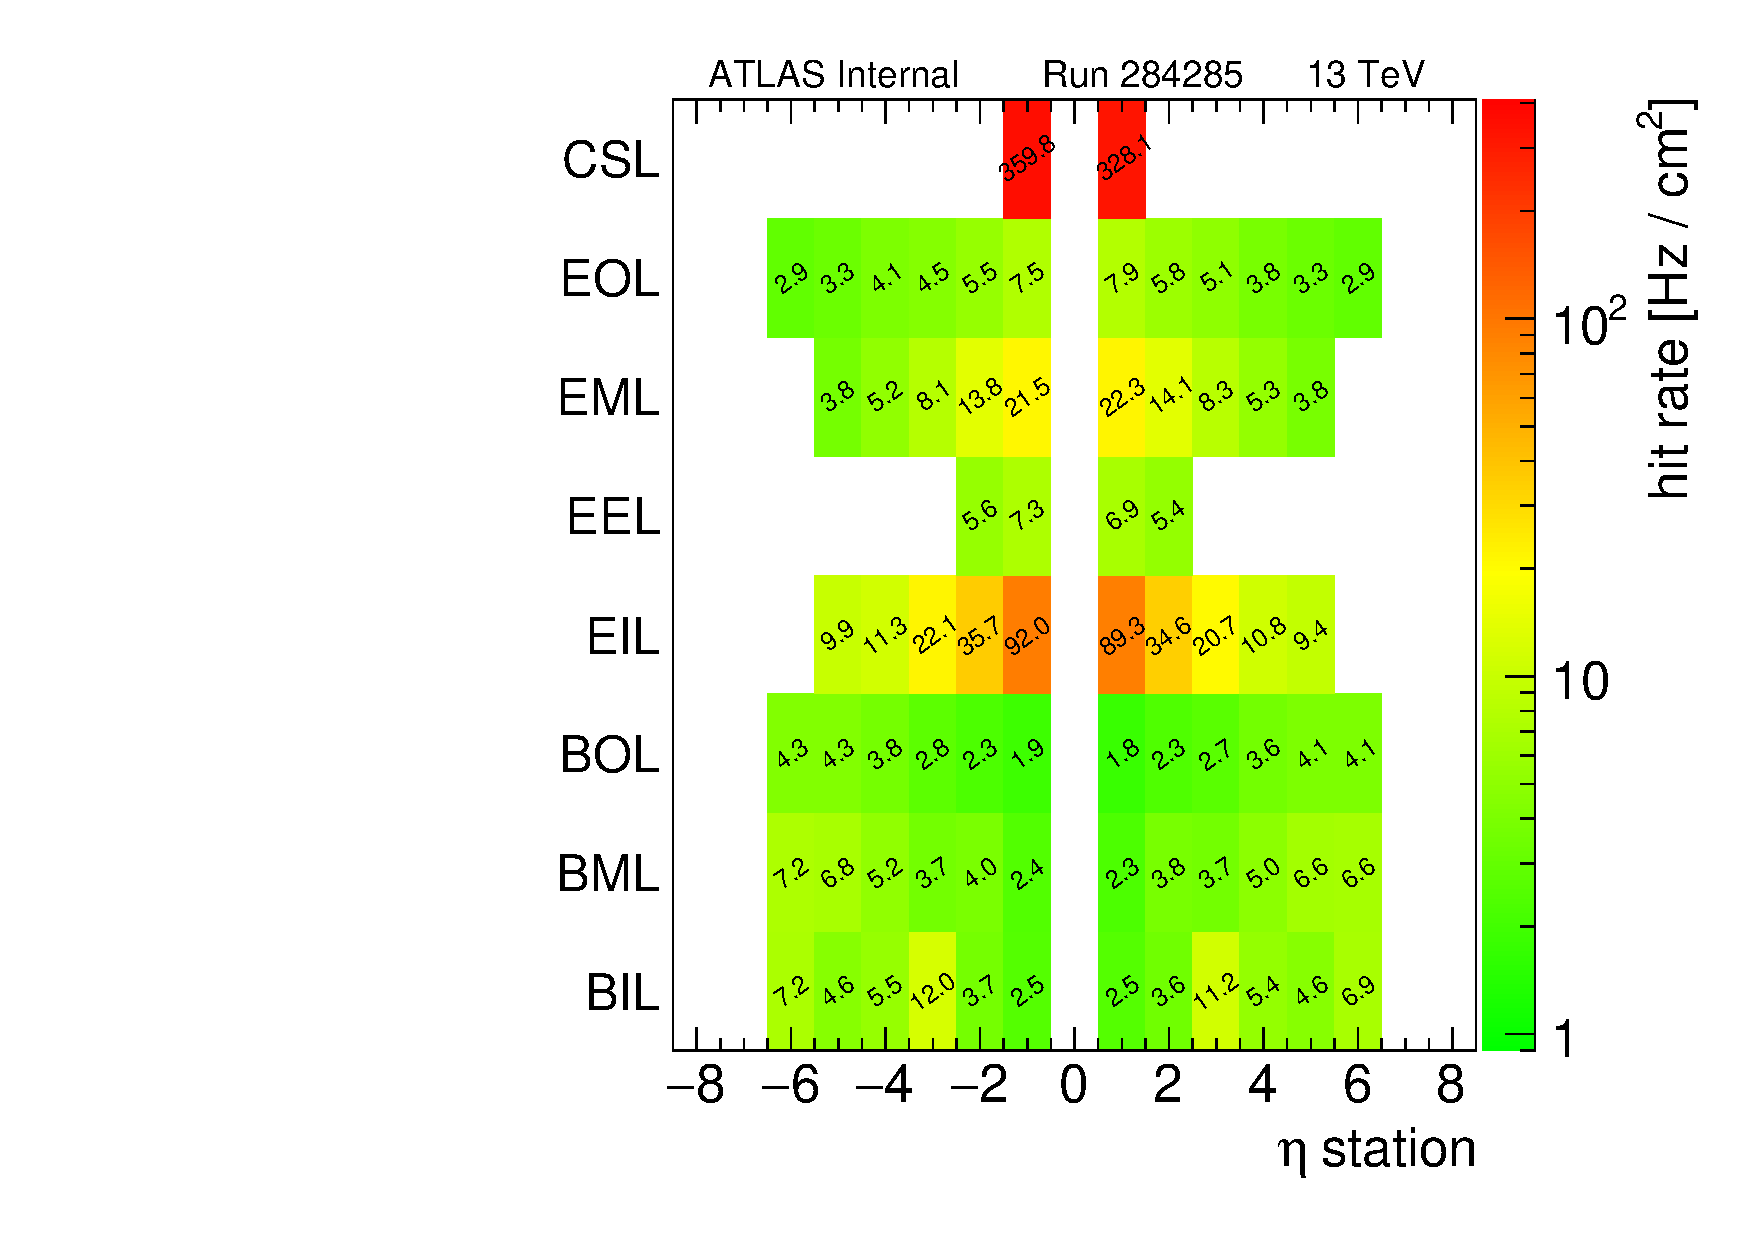
\includegraphics[width=0.45\textwidth]{./figures/rate_raw_vs_region_L_00284285.pdf}
    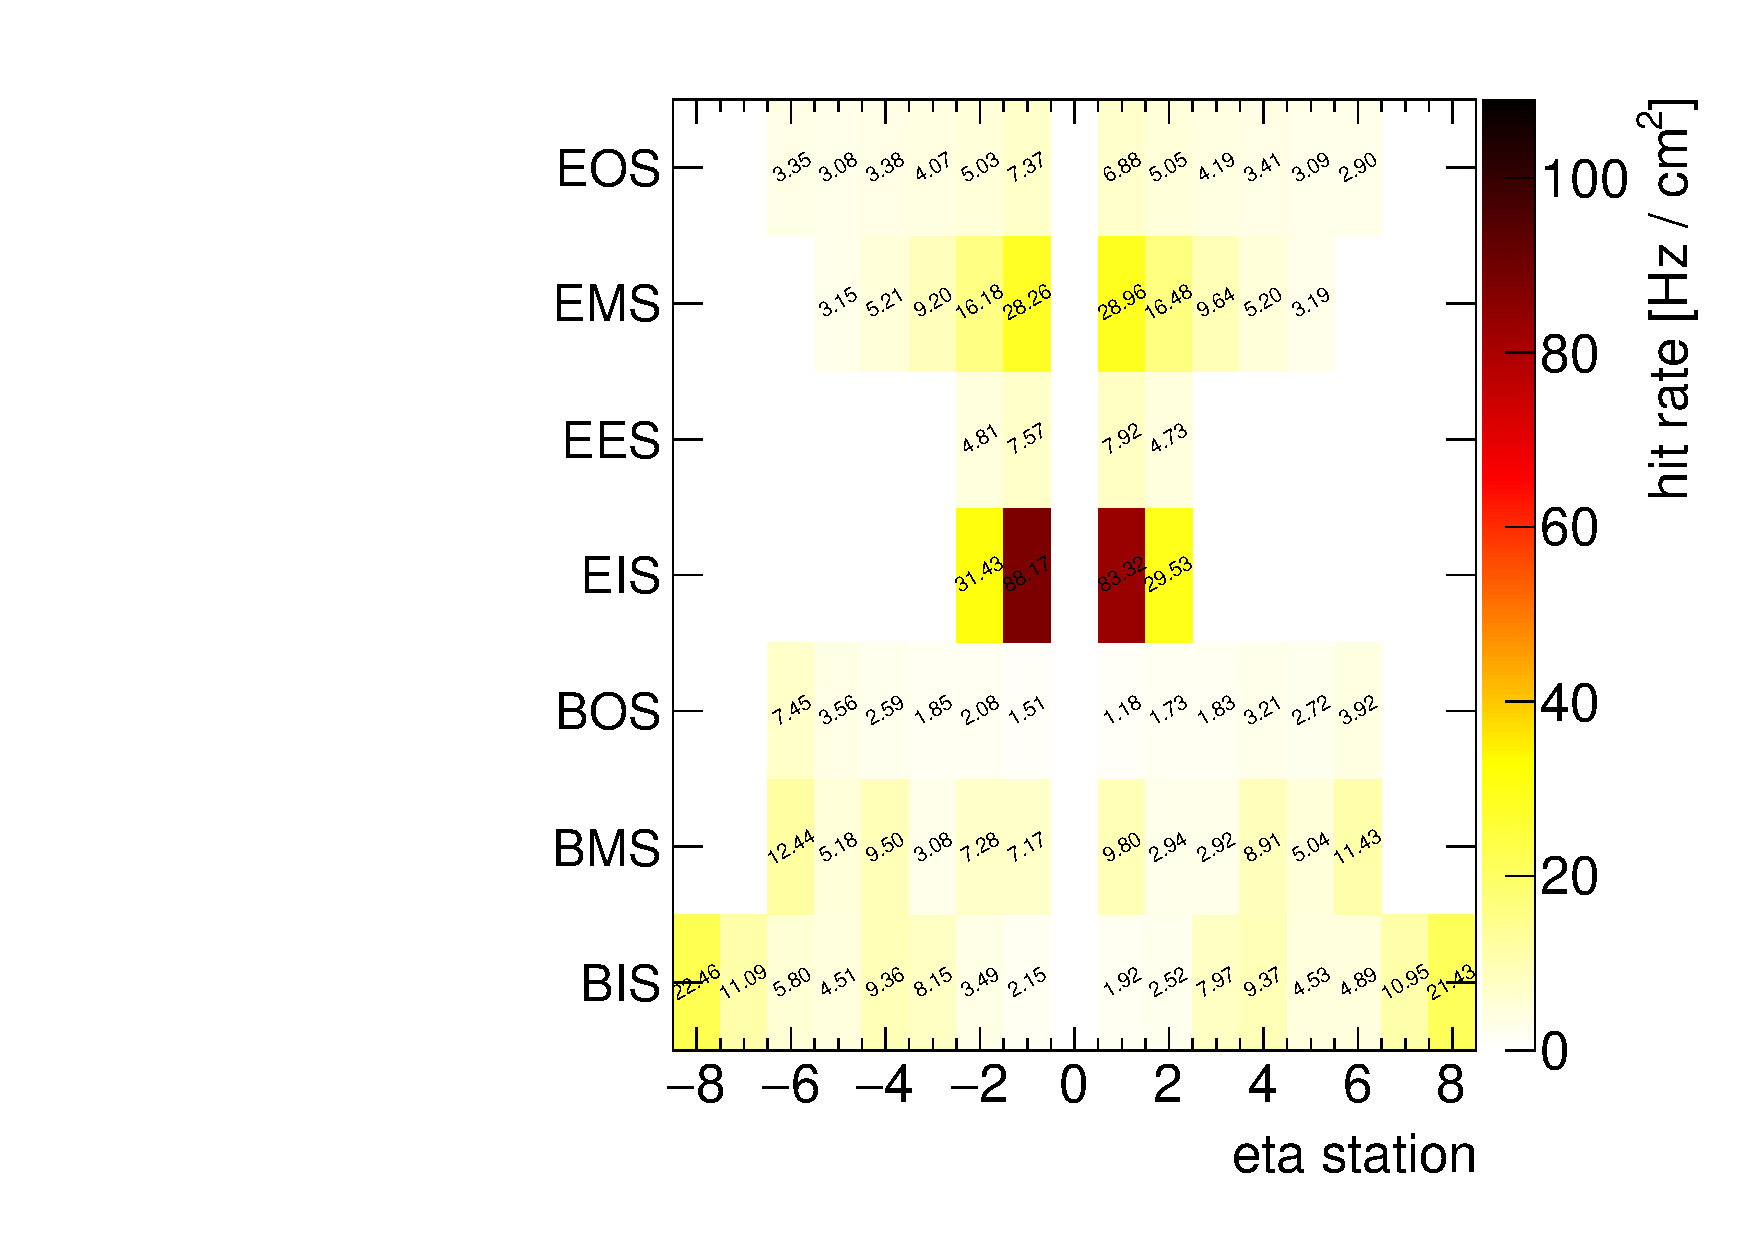
\includegraphics[width=0.45\textwidth]{./figures/rate_raw_vs_region_S_00284285.pdf}
    \caption{Total hit rate in the CSCs and MDTs in Run 284285 in the largest regions of the detector. The rates are split into large sectors (left) and small sectors (right). Positive eta stations indicate the $+z$ side of ATLAS, and negative eta stations indicate the $-z$ side.}
    \label{fig:hitrates-vs-region-raw}
  \end{center}
\end{figure}

The regions of the MDTs and CSCs with the highest rate are of special interest because the harsher conditions probe the data-taking capacity of the detectors. The hit rate as a function of instantaneous luminosity in this regions is measured to gauge the detector performance in the presence of increasing particle flux, since the instantaneous luminosity is linearly proportional to the number of interactions in a proton bunch crossing.

The hit rates for the CSC L and S chambers, MDT EIL1 and EIS1 chambers, and MDT EML1 and EMS1 chambers are shown as a function of the instantaneous luminosity in Figures~\ref{fig:hitrates-vs-lumi-csc-raw}, \ref{fig:hitrates-vs-lumi-mdt-ei1-raw}, and \ref{fig:hitrates-vs-lumi-mdt-em1-raw}, respectively. Linear fits are overlaid and provide a reasonable description of the data. The hit rates show strong dependence on the number of filled bunches in the LHC. The hit rates do not show non-linear behavior, such as saturation, at the highest instantaneous luminosity reached in 2015. This indicates robust MDT and CSC operation during 2015 data-taking.

\begin{figure}
  \begin{center}
    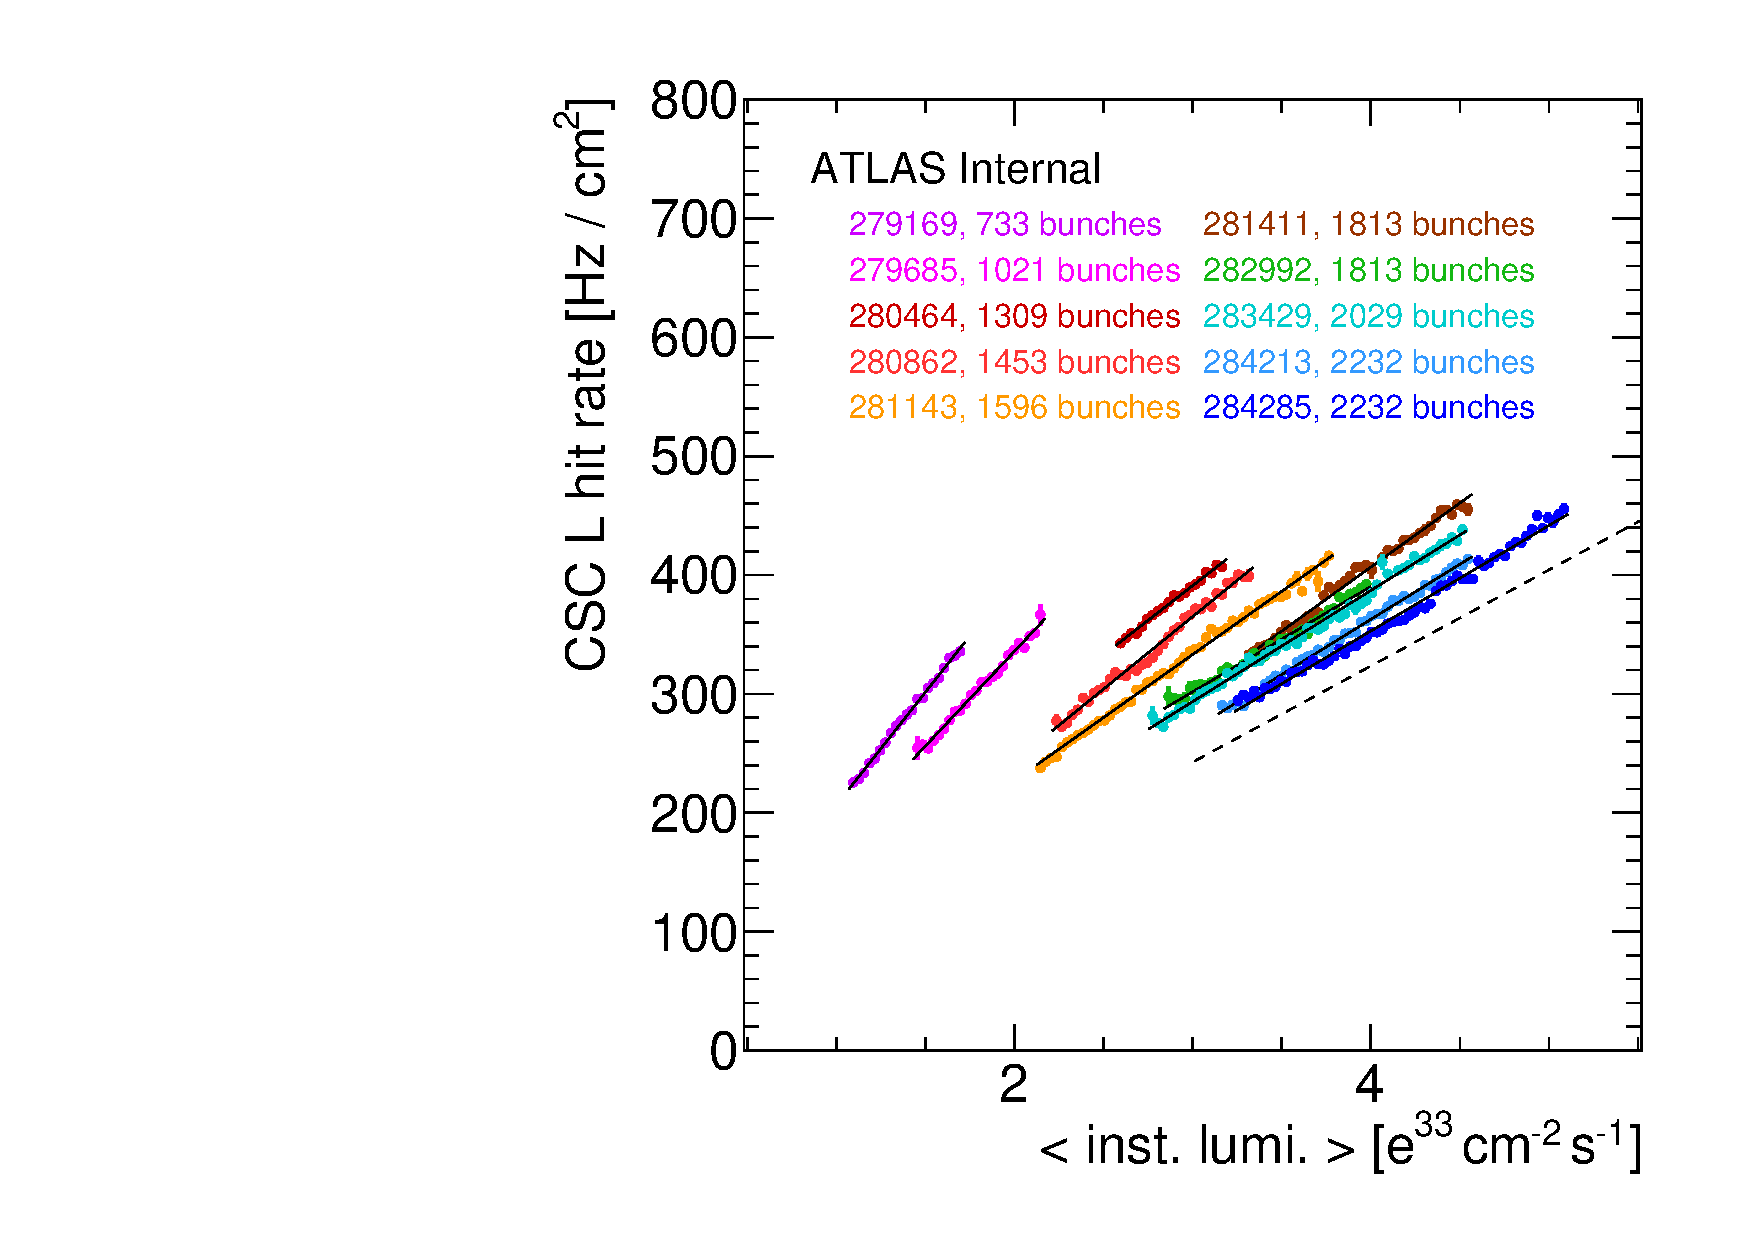
\includegraphics[width=0.45\textwidth]{./figures/rate_raw_vs_lumi_vs_evts_csc_CSL1_overlay.pdf}
    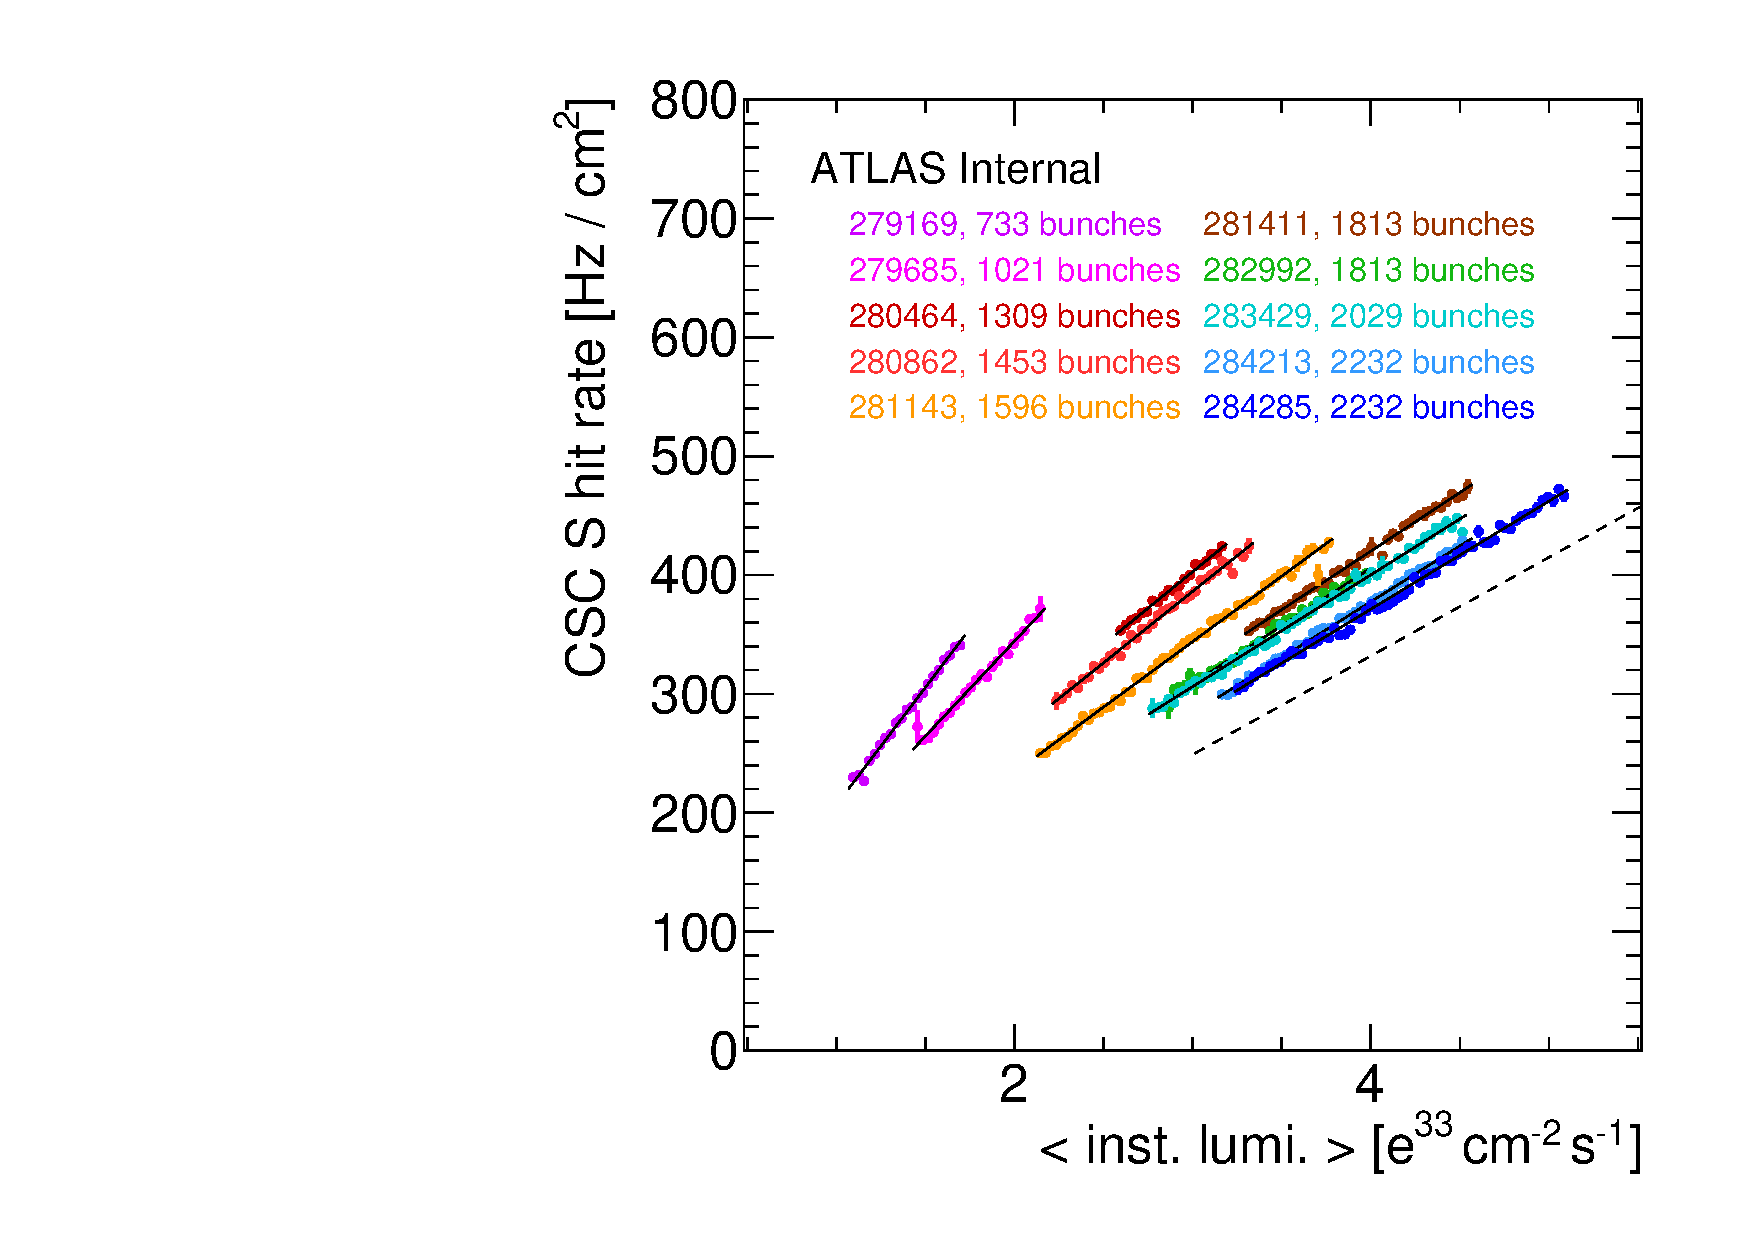
\includegraphics[width=0.45\textwidth]{./figures/rate_raw_vs_lumi_vs_evts_csc_CSS1_overlay.pdf}
    \caption{Total hit rate in the CSC large (left) and small (right) chambers as a function of instantaneous luminosity, for multiple runs.}
    \label{fig:hitrates-vs-lumi-csc-raw}
  \end{center}
\end{figure}

\begin{figure}
  \begin{center}
    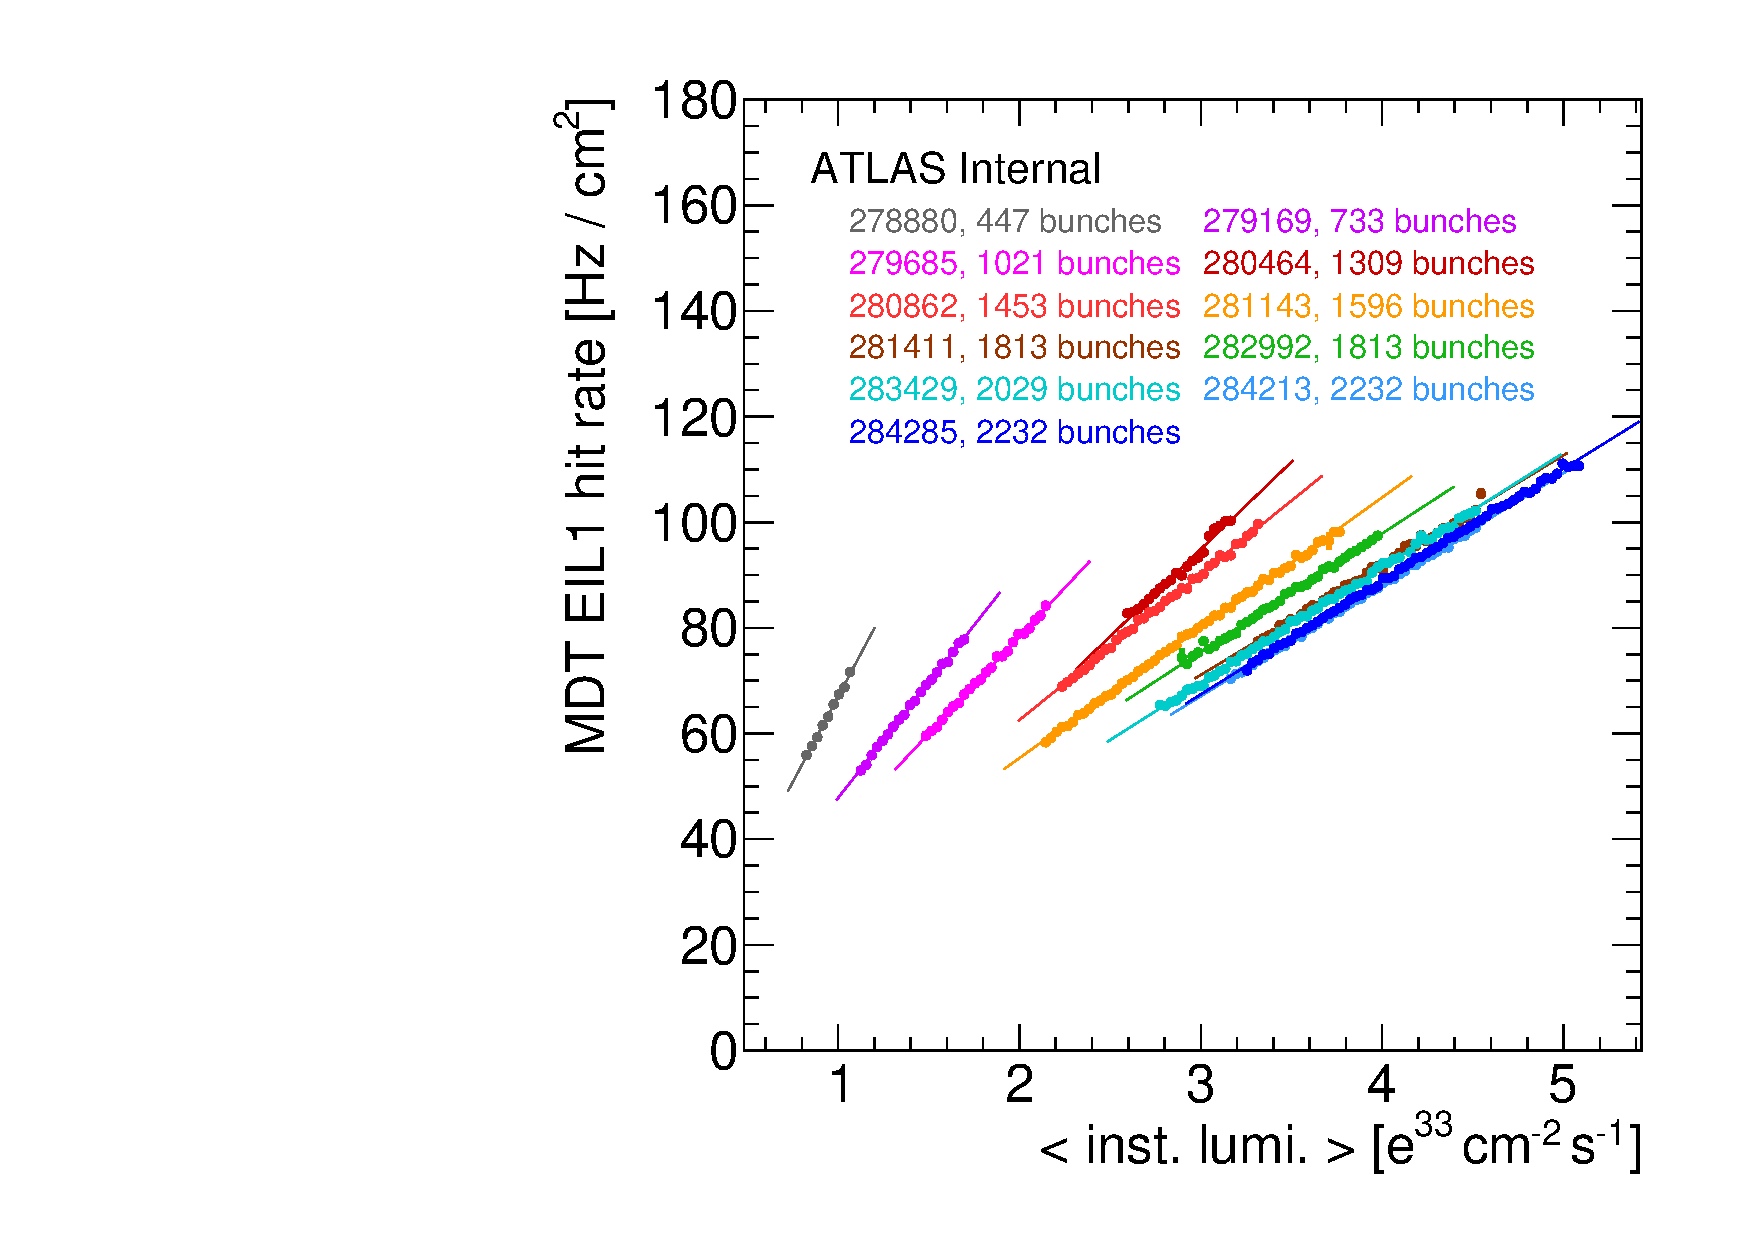
\includegraphics[width=0.45\textwidth]{./figures/rate_raw_vs_lumi_vs_evts_mdt_EIL1_overlay.pdf}
    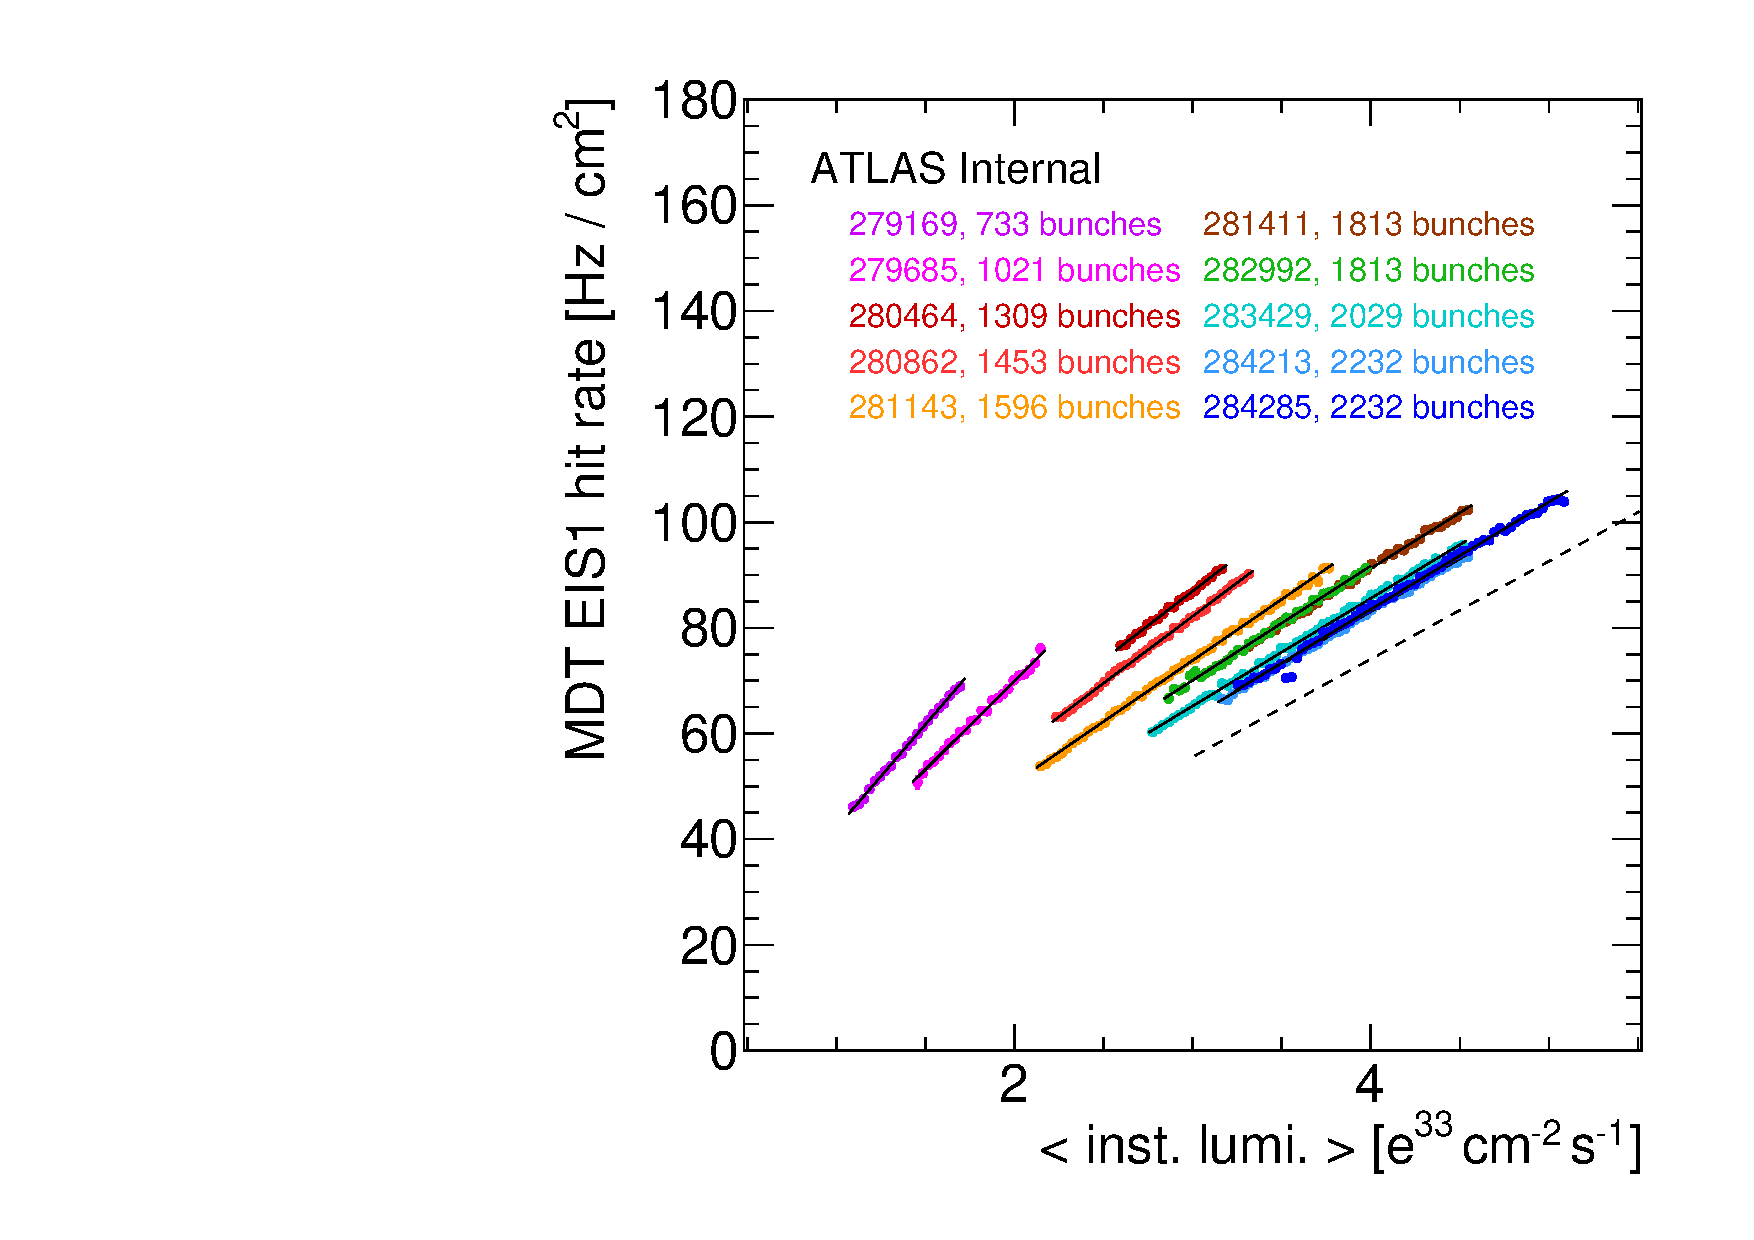
\includegraphics[width=0.45\textwidth]{./figures/rate_raw_vs_lumi_vs_evts_mdt_EIS1_overlay.pdf}
    \caption{Total hit rate in the MDT EI large (left) and small (right) chambers as a function of instantaneous luminosity, for multiple runs.}
    \label{fig:hitrates-vs-lumi-mdt-ei1-raw}
  \end{center}
\end{figure}

\begin{figure}
  \begin{center}
    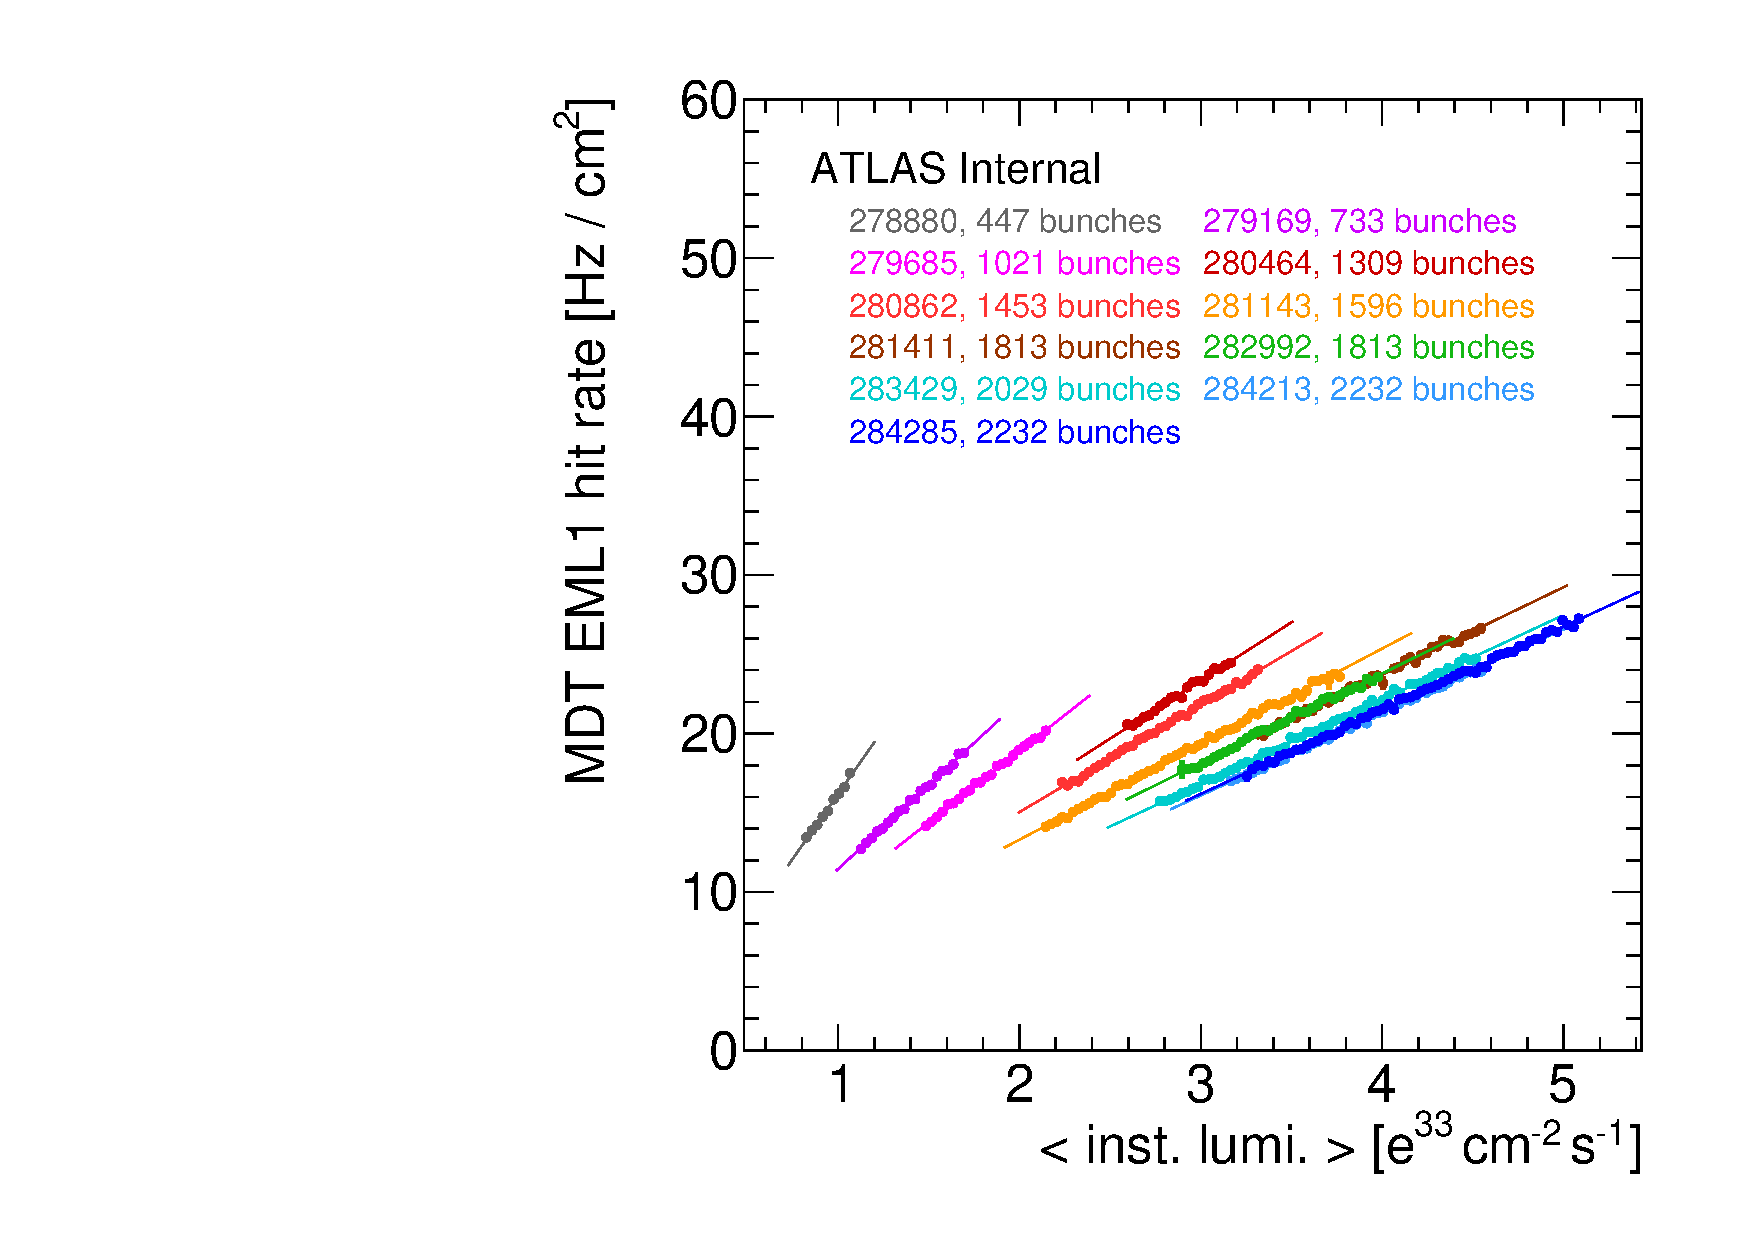
\includegraphics[width=0.45\textwidth]{./figures/rate_raw_vs_lumi_vs_evts_mdt_EML1_overlay.pdf}
    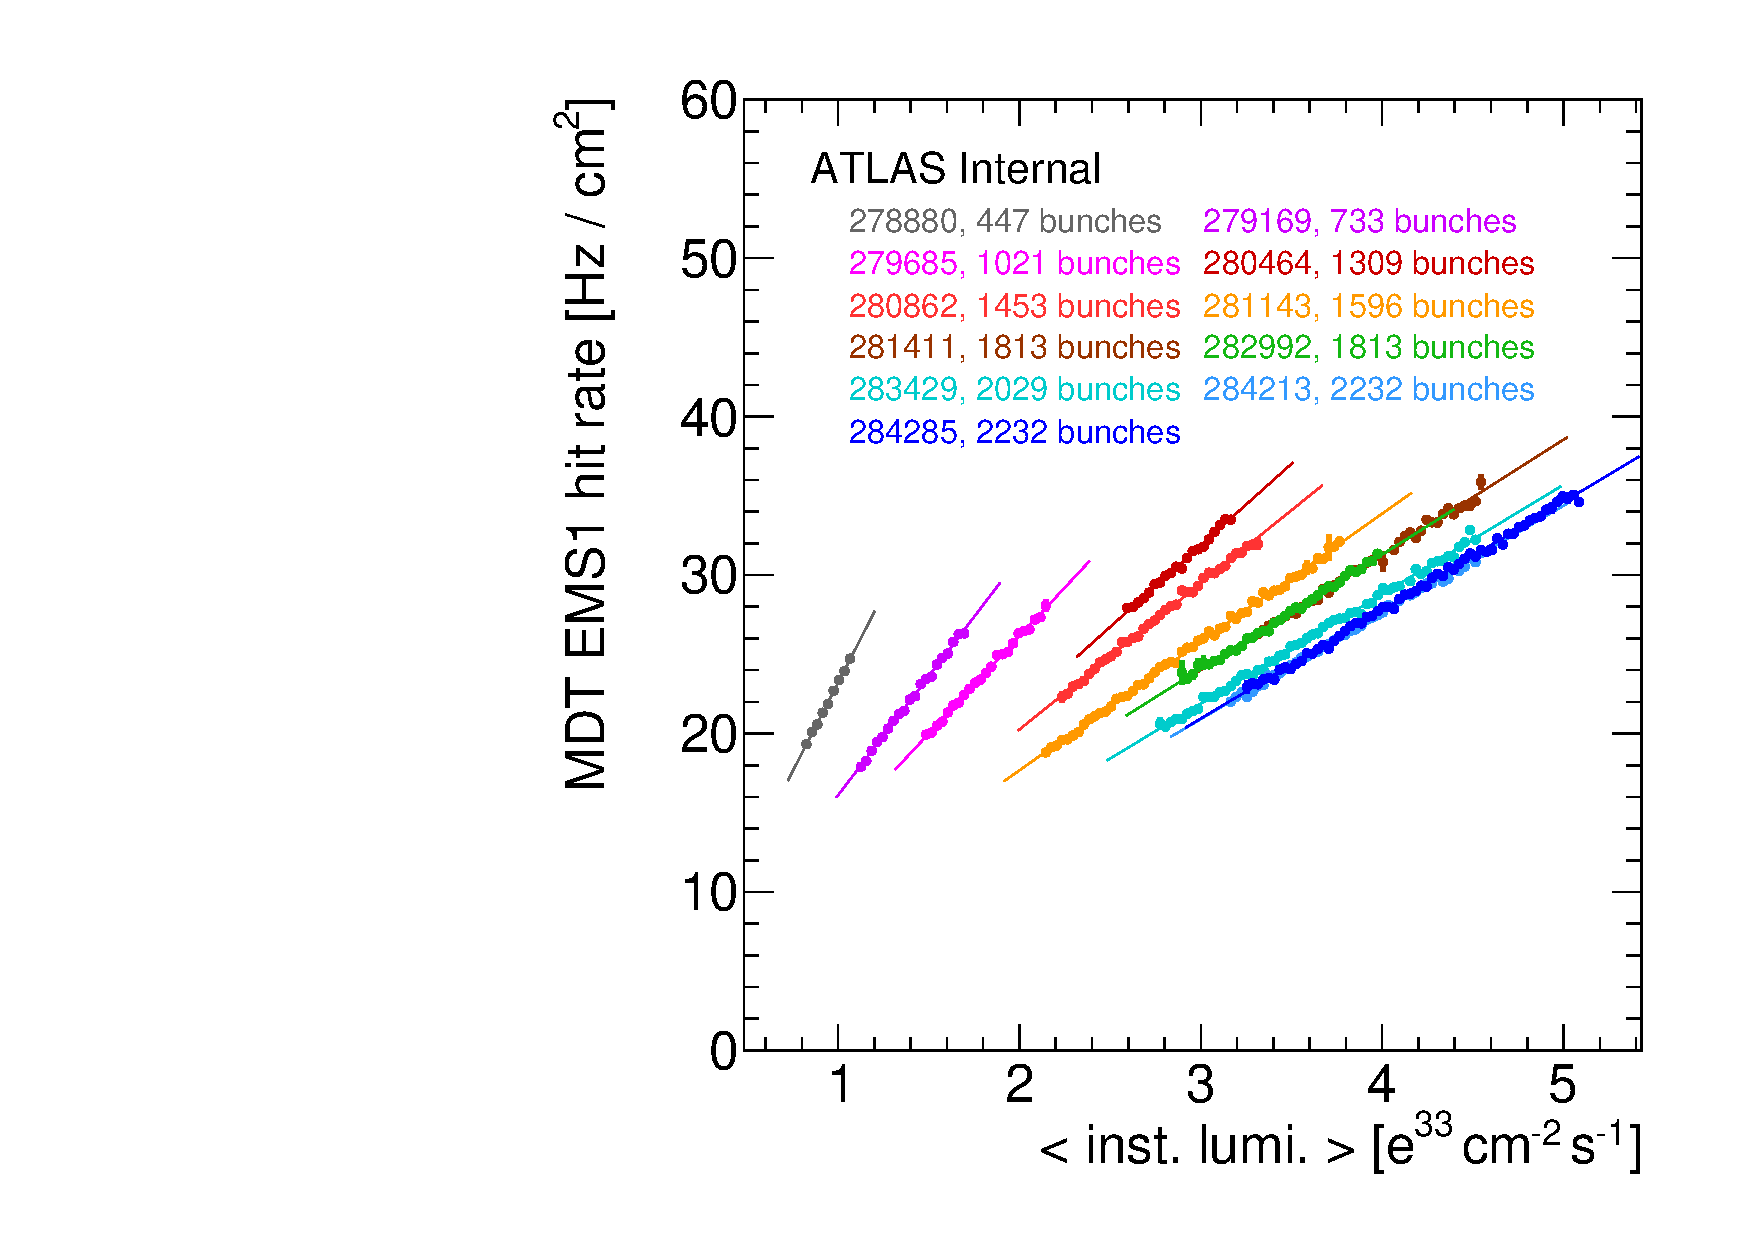
\includegraphics[width=0.45\textwidth]{./figures/rate_raw_vs_lumi_vs_evts_mdt_EMS1_overlay.pdf}
    \caption{Total hit rate in the MDT EM large (left) and small (right) chambers as a function of instantaneous luminosity, for multiple runs.}
    \label{fig:hitrates-vs-lumi-mdt-em1-raw}
  \end{center}
\end{figure}

In the endcap chambers, the hit rate depends significantly on the transverse distance $r$ from the beampipe. This is shown in Figure~\ref{fig:hitrates-vs-r-raw} for Run 284285 in the inner endcap, which includes CSC, MDT EIL1 and EIS1, and MDT EIL2 and EIS2 chambers. The CSC hit rates are as large as 800 $\text{Hz} / \text{cm}^2$ closest to the beampipe and as small as 150 $\text{Hz} / \text{cm}^2$ furthest from the beampipe. Exponential fits as a function of $r$ are overlaid and provide a reasonable description of the data. A comparison of the average and peak hit rates in the CSCs are sumarized in Table~\ref{tab:hitrates-vs-r-raw}.

\begin{figure}
  \begin{center}
    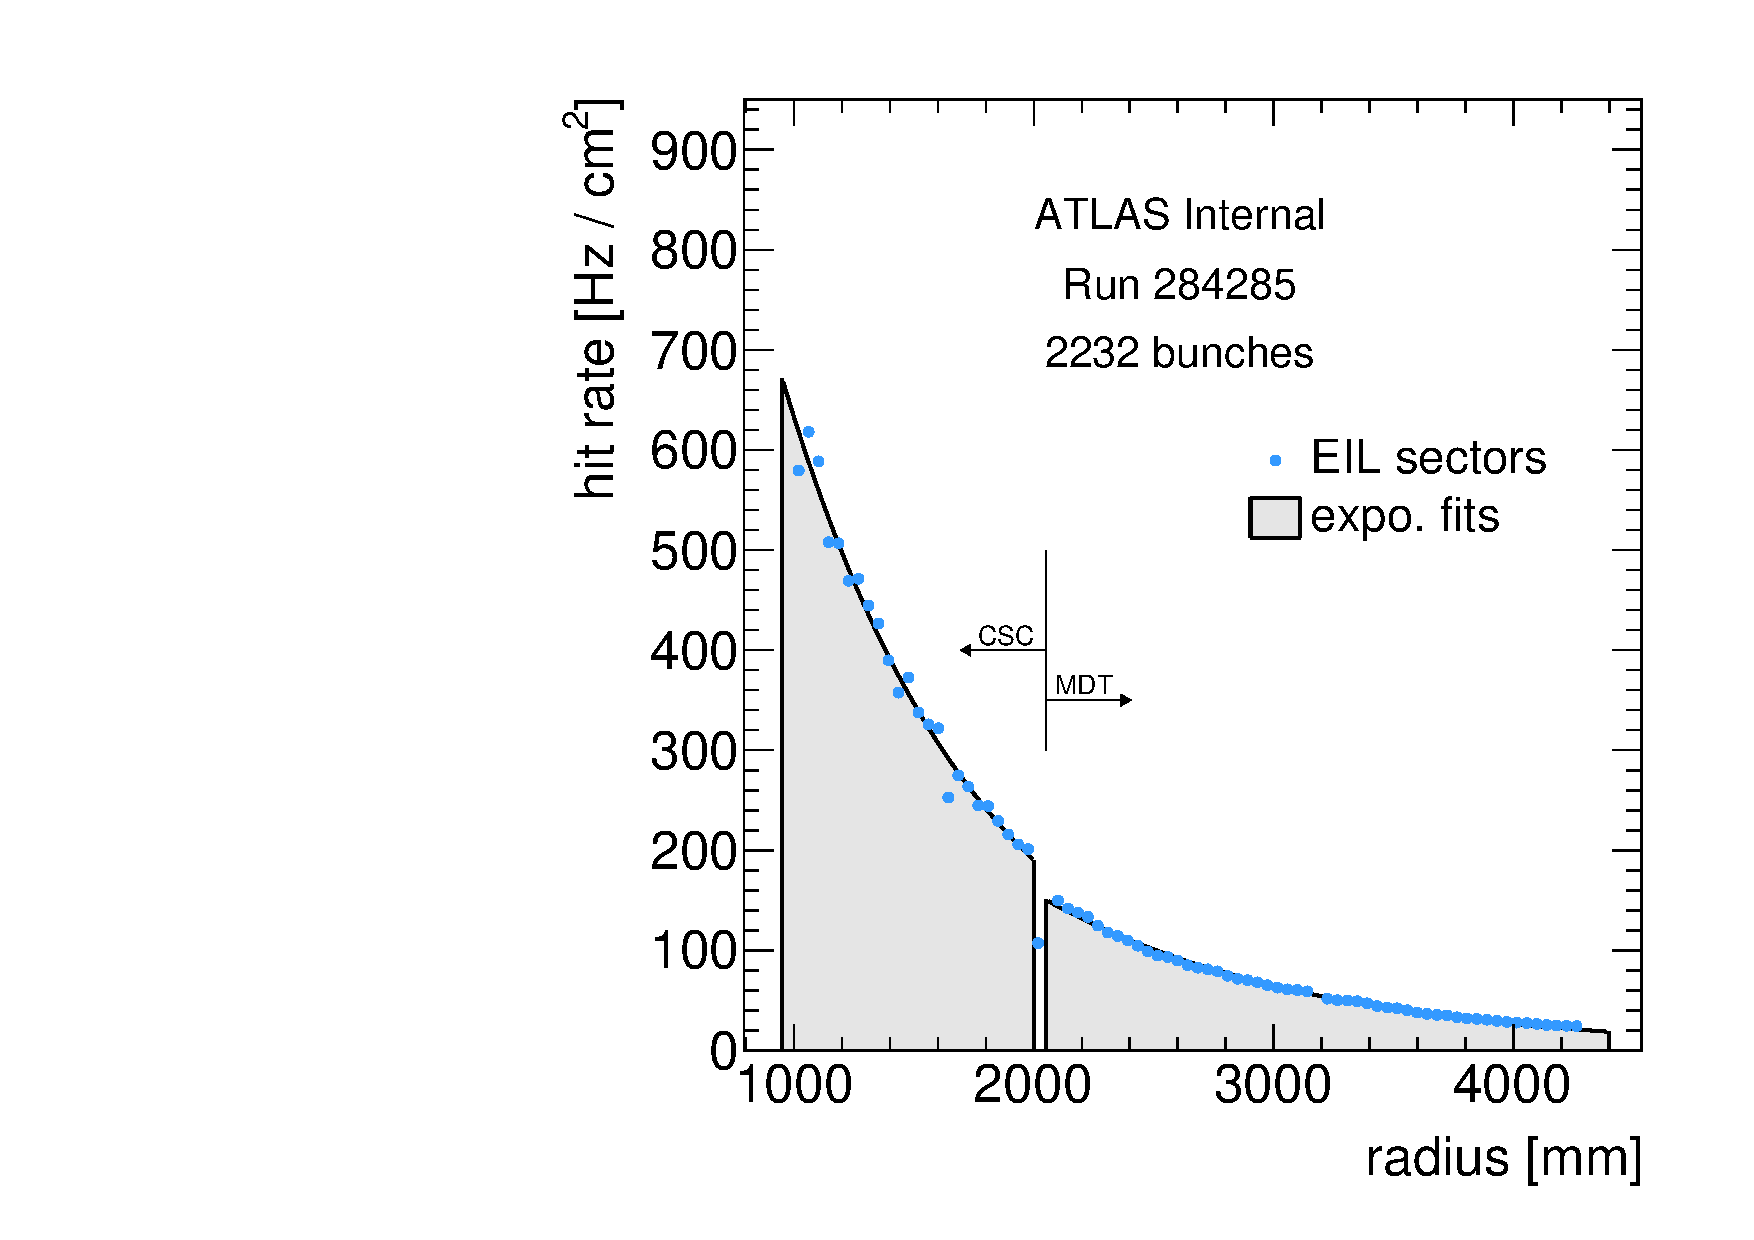
\includegraphics[width=0.45\textwidth]{./figures/rate_raw_vs_r_EIL_00284285.pdf}
    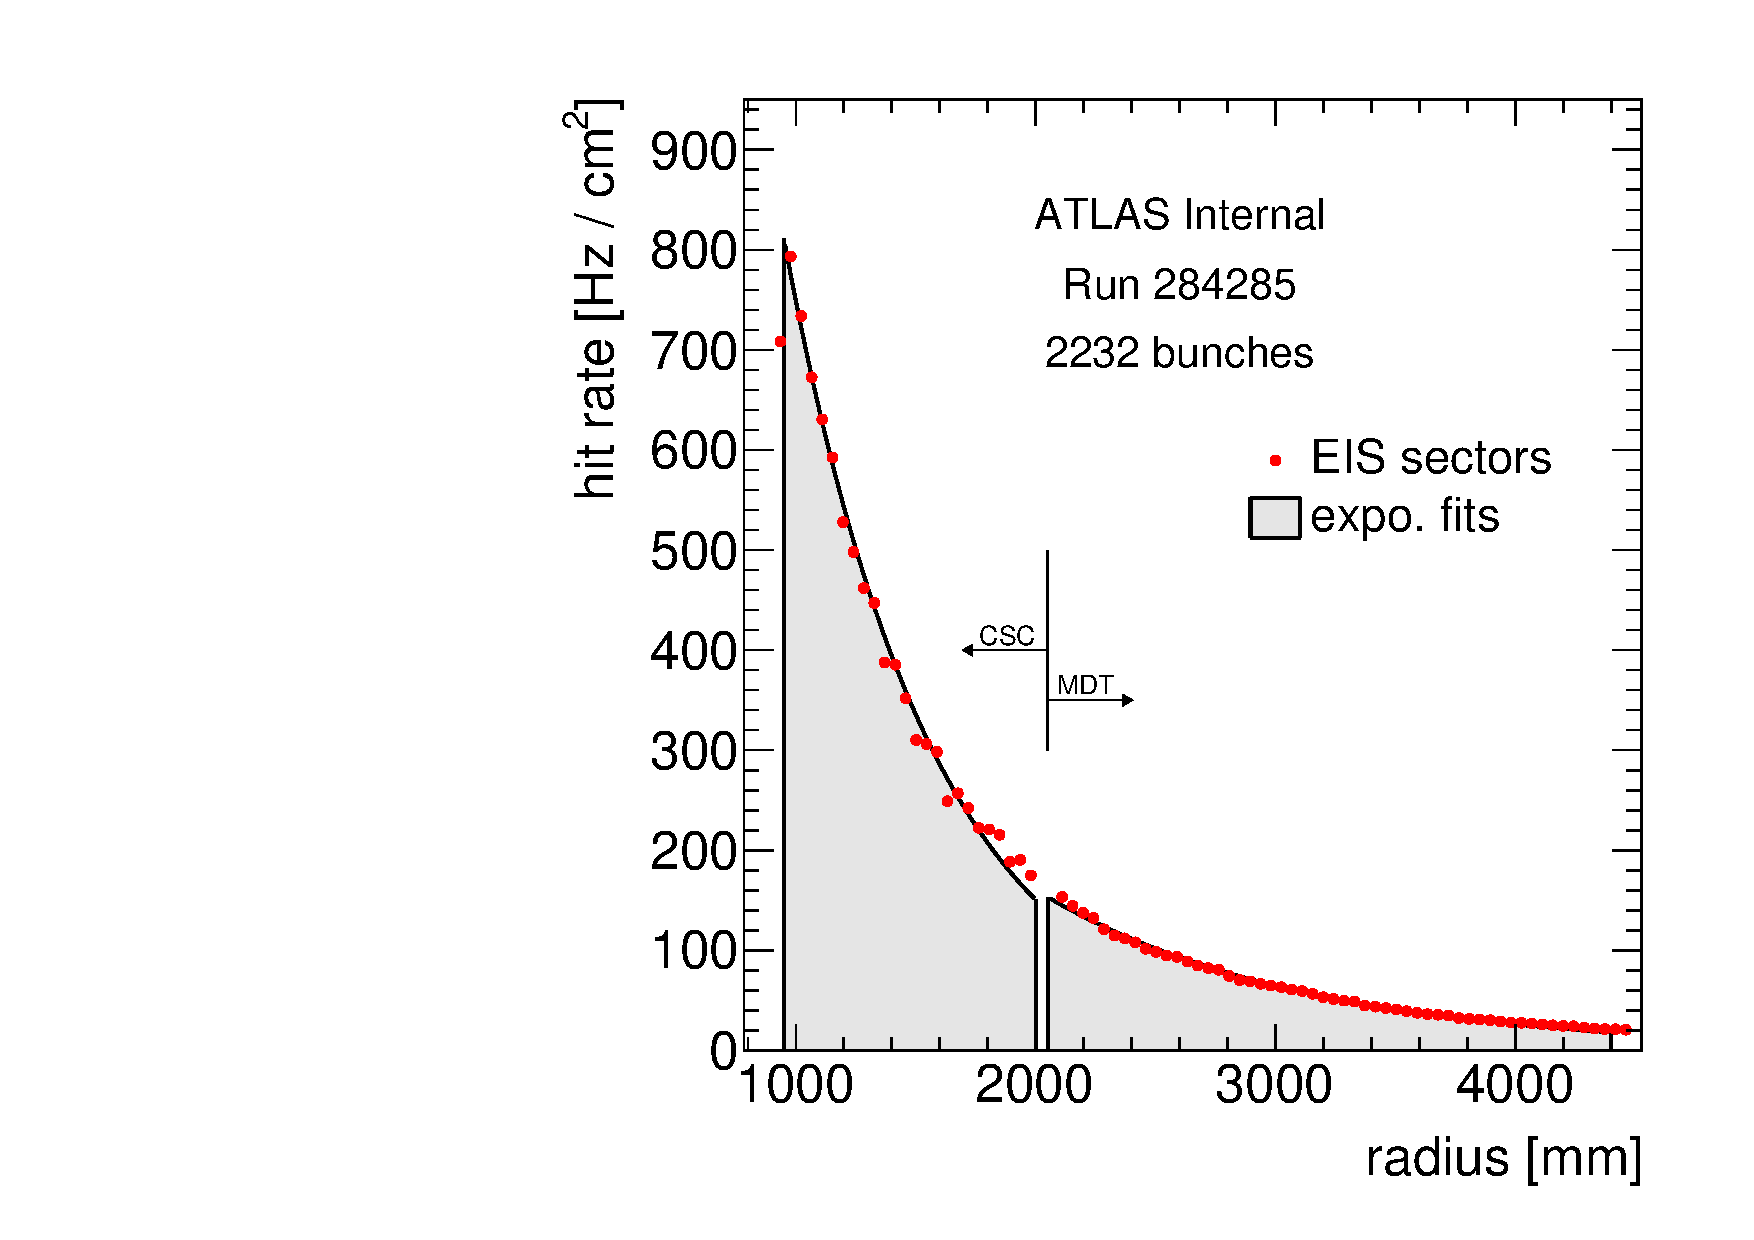
\includegraphics[width=0.45\textwidth]{./figures/rate_raw_vs_r_EIS_00284285.pdf}
    \caption{Total hit rate as a function of the transverse distance from the beam pipe in the small wheel, for large (left) and small (right) sectors, in Run 284285.}
    \label{fig:hitrates-vs-r-raw}
  \end{center}
\end{figure}

\newcommand*{\hspsix}{\hspace*{0.6cm}}

\begin{table}
  \begin{center}
    \renewcommand{\arraystretch}{1.4}
    \begin{tabular}{c|c|c|c|c}
      \multicolumn{2}{c|}{}                                             & \multicolumn{2}{c|}{\rate}                   & \multicolumn{1}{c}{} \\
      \hspsix region \hspsix & expo. fit                                & \hspsix average \hspsix & peak: smallest $r$ & peak / average \\
      \hline\hline
      CSC L                  & $e^{\ 7.65\ -\ 1.20\cdot r \text{ [m]}}$ & 344                     & 668                & 1.94 \\
      CSC S                  & $e^{\ 8.22\ -\ 1.61\cdot r \text{ [m]}}$ & 360                     & 803                & 2.23 \\
    \end{tabular}
    \caption{Comparison of the CSC chamber average hit rate with the hit rate closest to the beampipe in Run 284285. The average luminosity in Run 284285 is $\mathcal{L}=4.1\times10^{33}$.}
    \label{tab:hitrates-vs-r-raw}
  \end{center}
\end{table}


\section{Extrapolations to higher luminosity}
\label{sec:extrapolations}

Future runs of the LHC expect to deliver significantly higher instantaneous luminosity than current operations. To cope with these harsher data-taking conditions, upgrades to the muon spectrometer are planned. In Long Shutdown 2 which is scheduled to start in 2018, the current endcap small wheels will be replaced by the New Small Wheels equipped with small Thin Gap Chambers (sTGC) and MicroMegas (MM) detectors. In Long Shutdown 3, which is scheduled to start near 2022, an additional round of upgrades is now being planned as the LHC will enter its high-luminosity phase, the HL-LHC.

% the MDT electronics are being considered for replacement, and additional coverage for the barrel muon trigger system is under consideration.

A crucial ingredient in the planning of these upgrades is the hit rate of incident particles the detectors are expected to receive. This section presents an expected rate in the hottest regions of the MS as extrapolated from data-taking in 2015. This extrapolation does not address potential changes in the ATLAS shielding or the beam pipe, or the particle sensitivity of future detector technologies, both of which can have a large effect and must be characterized with simulation. The hottest regions of the MS in 2015 data are the innermost regions of the endcap inner small wheel (CSC L, CSC S, MDT EIL1, MDT EIS1) and endcap middle big wheel (EML1, EMS1).

The hit rates presented in Section~\ref{sec:hitrates} of the note include all hits reported by the detectors, including those from electronic noise. The contribution from electronic noise is detector-dependent, hence the inclusive hit rate may be less useful for projecting to future LHC conditions because new detectors (sTGC, MM) will be deployed in the NSW. The projections are split into two parts to address this. First, the inclusive hit rates are projected and can be considered an upper-bound of the future rates. Second, hit rates with hit quality criteria cuts (\textit{ADC cuts}) are projected, which remove a large fraction of electronic noise while maintaining good efficiency for hits from incident particles. This is a more accurate reflection of the conditions for future MS detectors, though an unfolding to particle fluxes is still not attempted. Here, the criteria for suppressing electronic noise are at least 50 ADC counts for an MDT tube and at least 100 ADC counts for the highest-ADC strip in a CSC cluster. The MDT (CSC) quality criteria is assumed to be fully (78.9\%) efficient for incident charged particles.

The predictions are performed by considering the hit rates in 2015 data-taking as a function of the instantaneous luminosity, fitting the linear dependence, and extrapolating to higher luminosity. These rates are shown in Section~\ref{sec:hitrates} with linear fits overlaid, for the inclusive hit rates.

The parameters of the linear fit depend on the number of filled bunches in the LHC, as expected. The maximum number of filled bunches in 2015 is 2232 bunches, whereas Run 3 of the LHC is expected to fill at most 2808 bunches, and the HL-LHC is expected to fill at most 3564 bunches. To extrapolate to more filled bunches, the fitted slopes are considered for 2015 runs with as few as 447 filled bunches and as many as 2232 bunches, and the dependency is extracted by fitting this spectrum to a first-order inverse power law, as shown in Figure~\ref{fig:extrapolations-slope-vs-bunches-raw} with vertical lines at 2808 and 3564 filled bunches. The fitted slopes are the same as reported in Figures~\ref{fig:hitrates-vs-lumi-csc-raw}, \ref{fig:hitrates-vs-lumi-mdt-ei1-raw}, and \ref{fig:hitrates-vs-lumi-mdt-em1-raw}. The same procedure is followed for the projected hit rates with ADC cuts.

\begin{figure}
  \begin{center}
    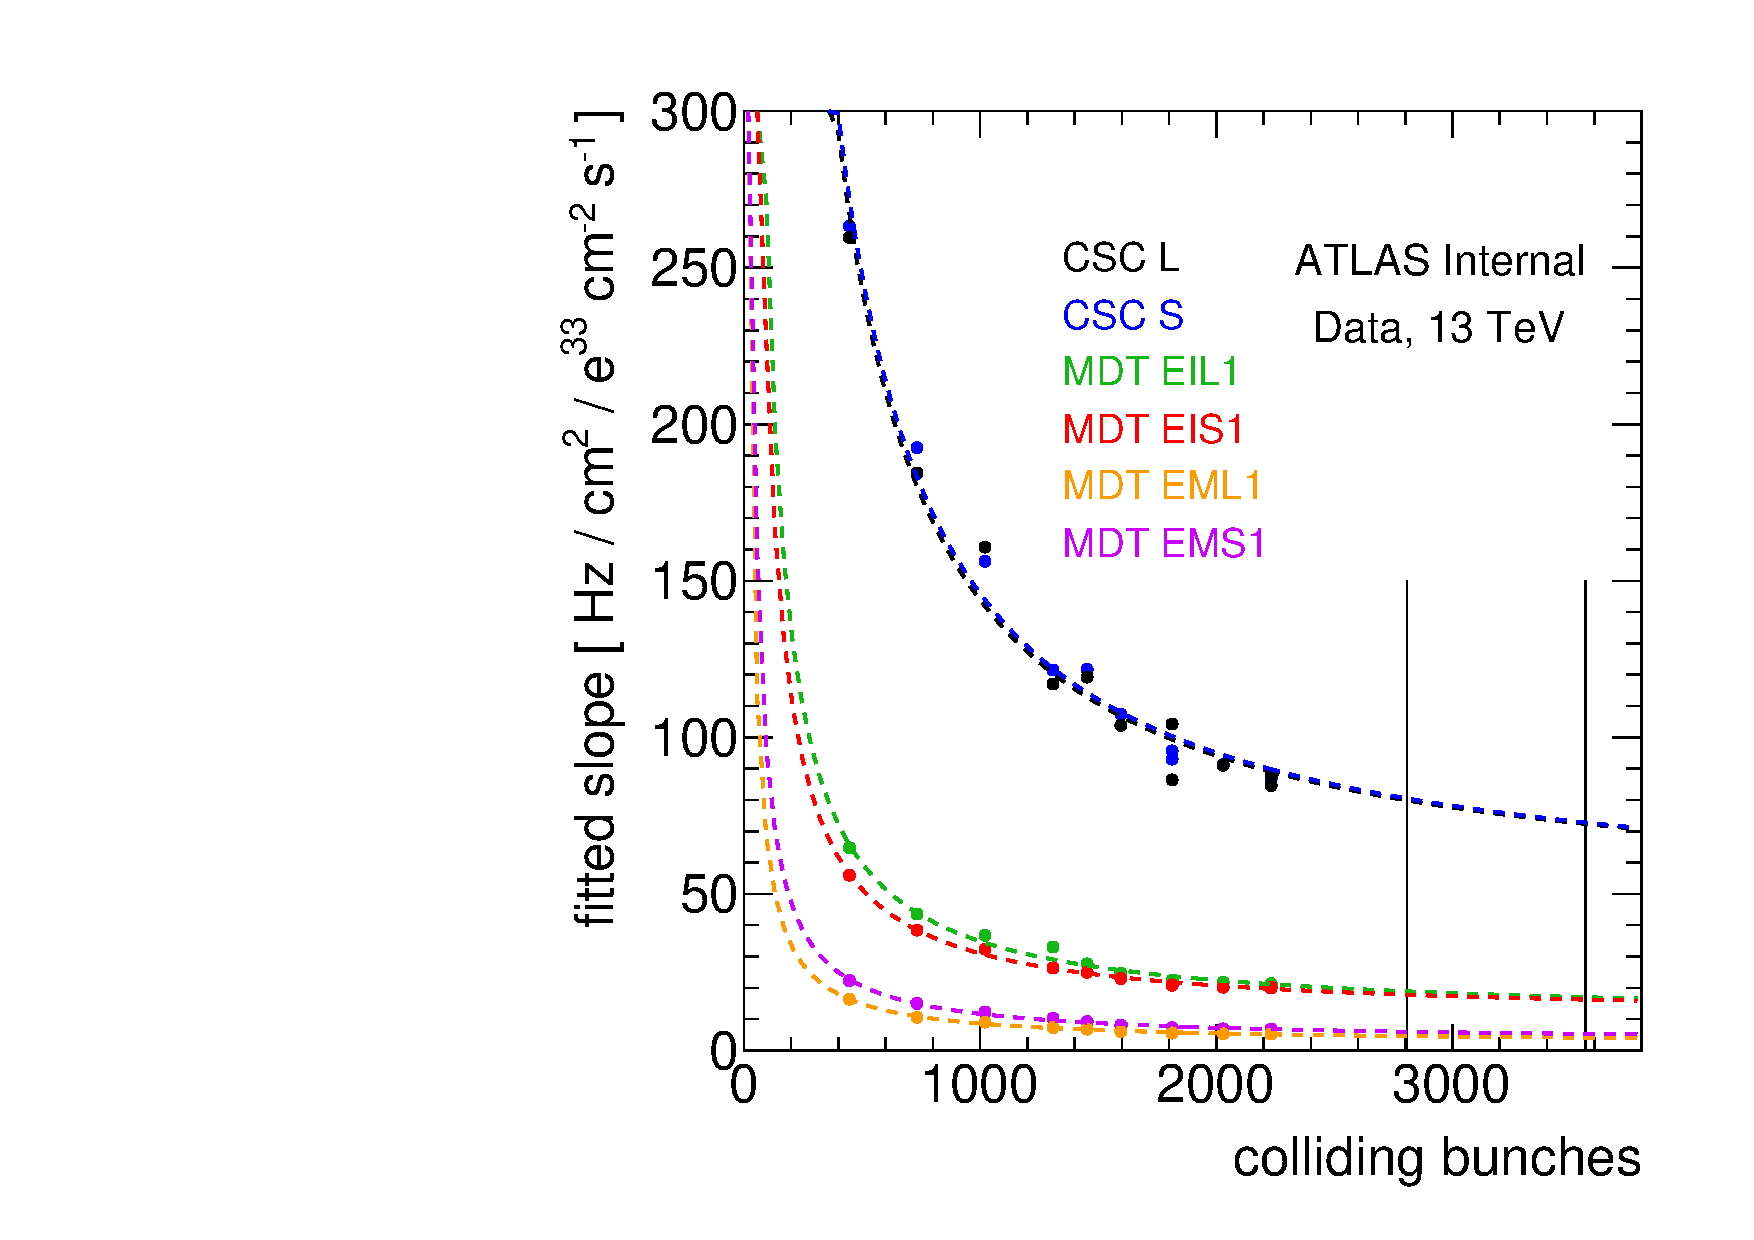
\includegraphics[width=0.45\textwidth]{./figures/slope_vs_bunches_raw_lin.pdf}
    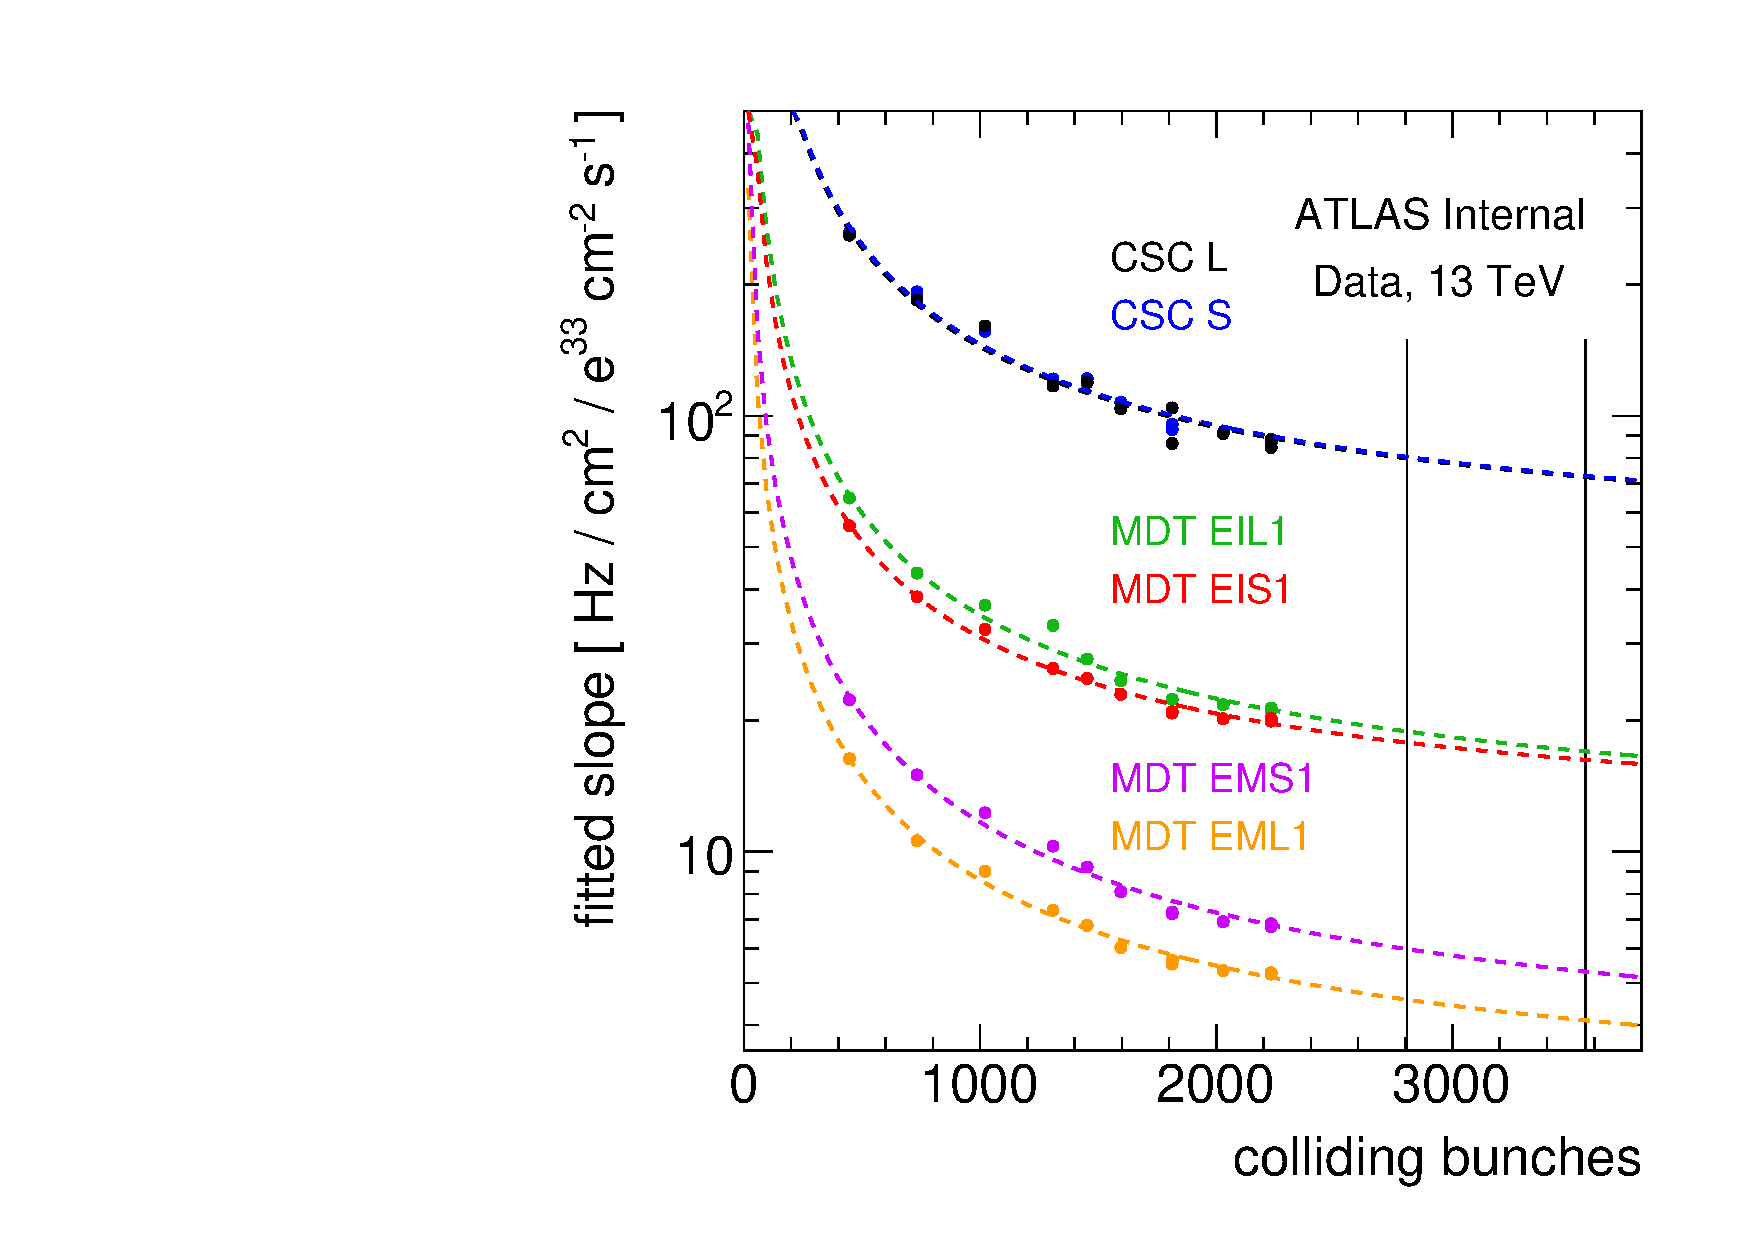
\includegraphics[width=0.45\textwidth]{./figures/slope_vs_bunches_raw_log.pdf}
    \caption{The fitted slope for inclusive hit rates as a function of the number of colliding bunches for various runs in the hottest MDT and CSC chambers, shown with linear (left) and logarithmic (right) scale. The spectra are fitted to $A + B/x$, where $x$ is the number of bunches.}
    \label{fig:extrapolations-slope-vs-bunches-raw}
  \end{center}
\end{figure}

This fit gives parameters for the linear dependence of hit rate on instantaneous luminosity at more filled bunches than was reached in 2015. The projected inclusive hit rates for the hottest chambers of the MS are shown in Figure~\ref{fig:extrapolations-hitrates-raw}. The large (L) and small (S) sectors of a given detector region have similar projected hit rates.

\begin{figure}
  \begin{center}
    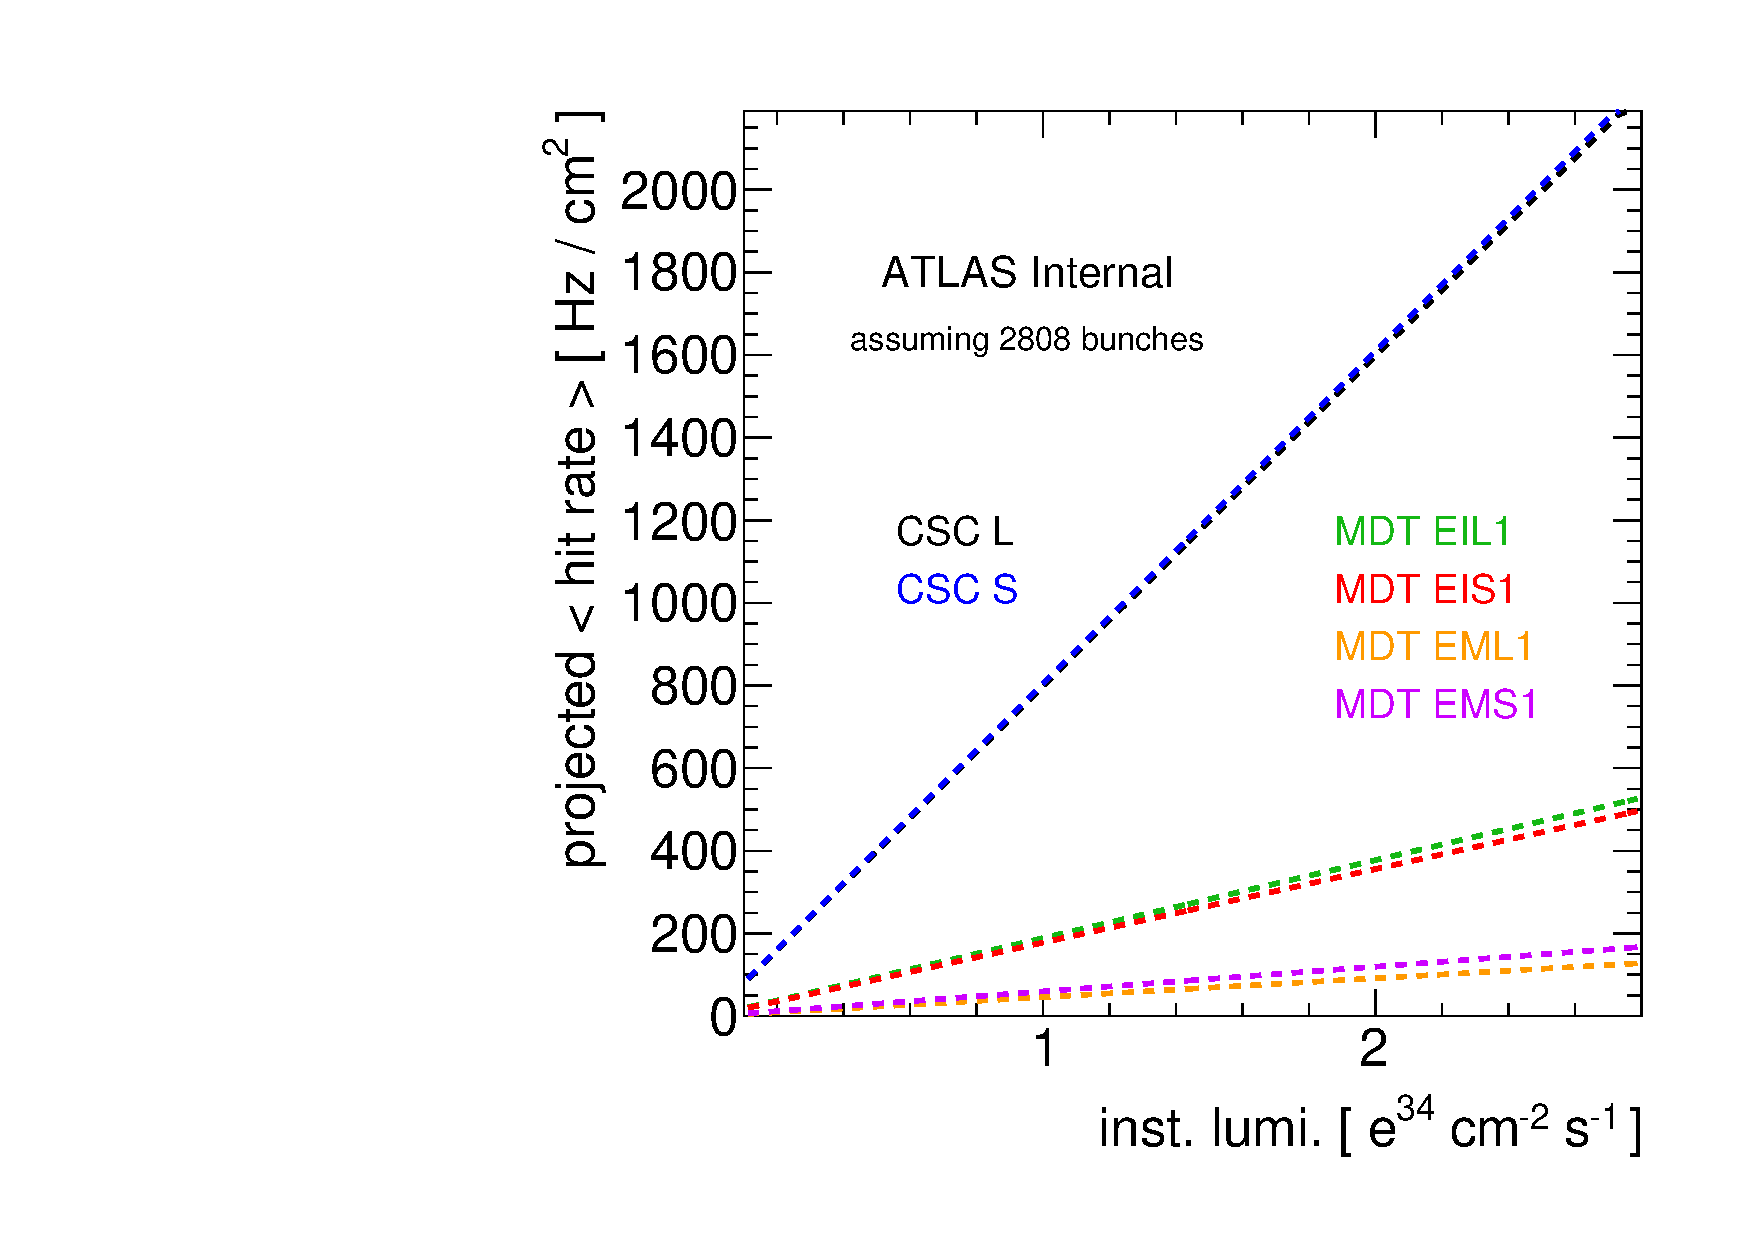
\includegraphics[width=0.45\textwidth]{./figures/extrapolate_vs_lumi_raw_2808.pdf}
    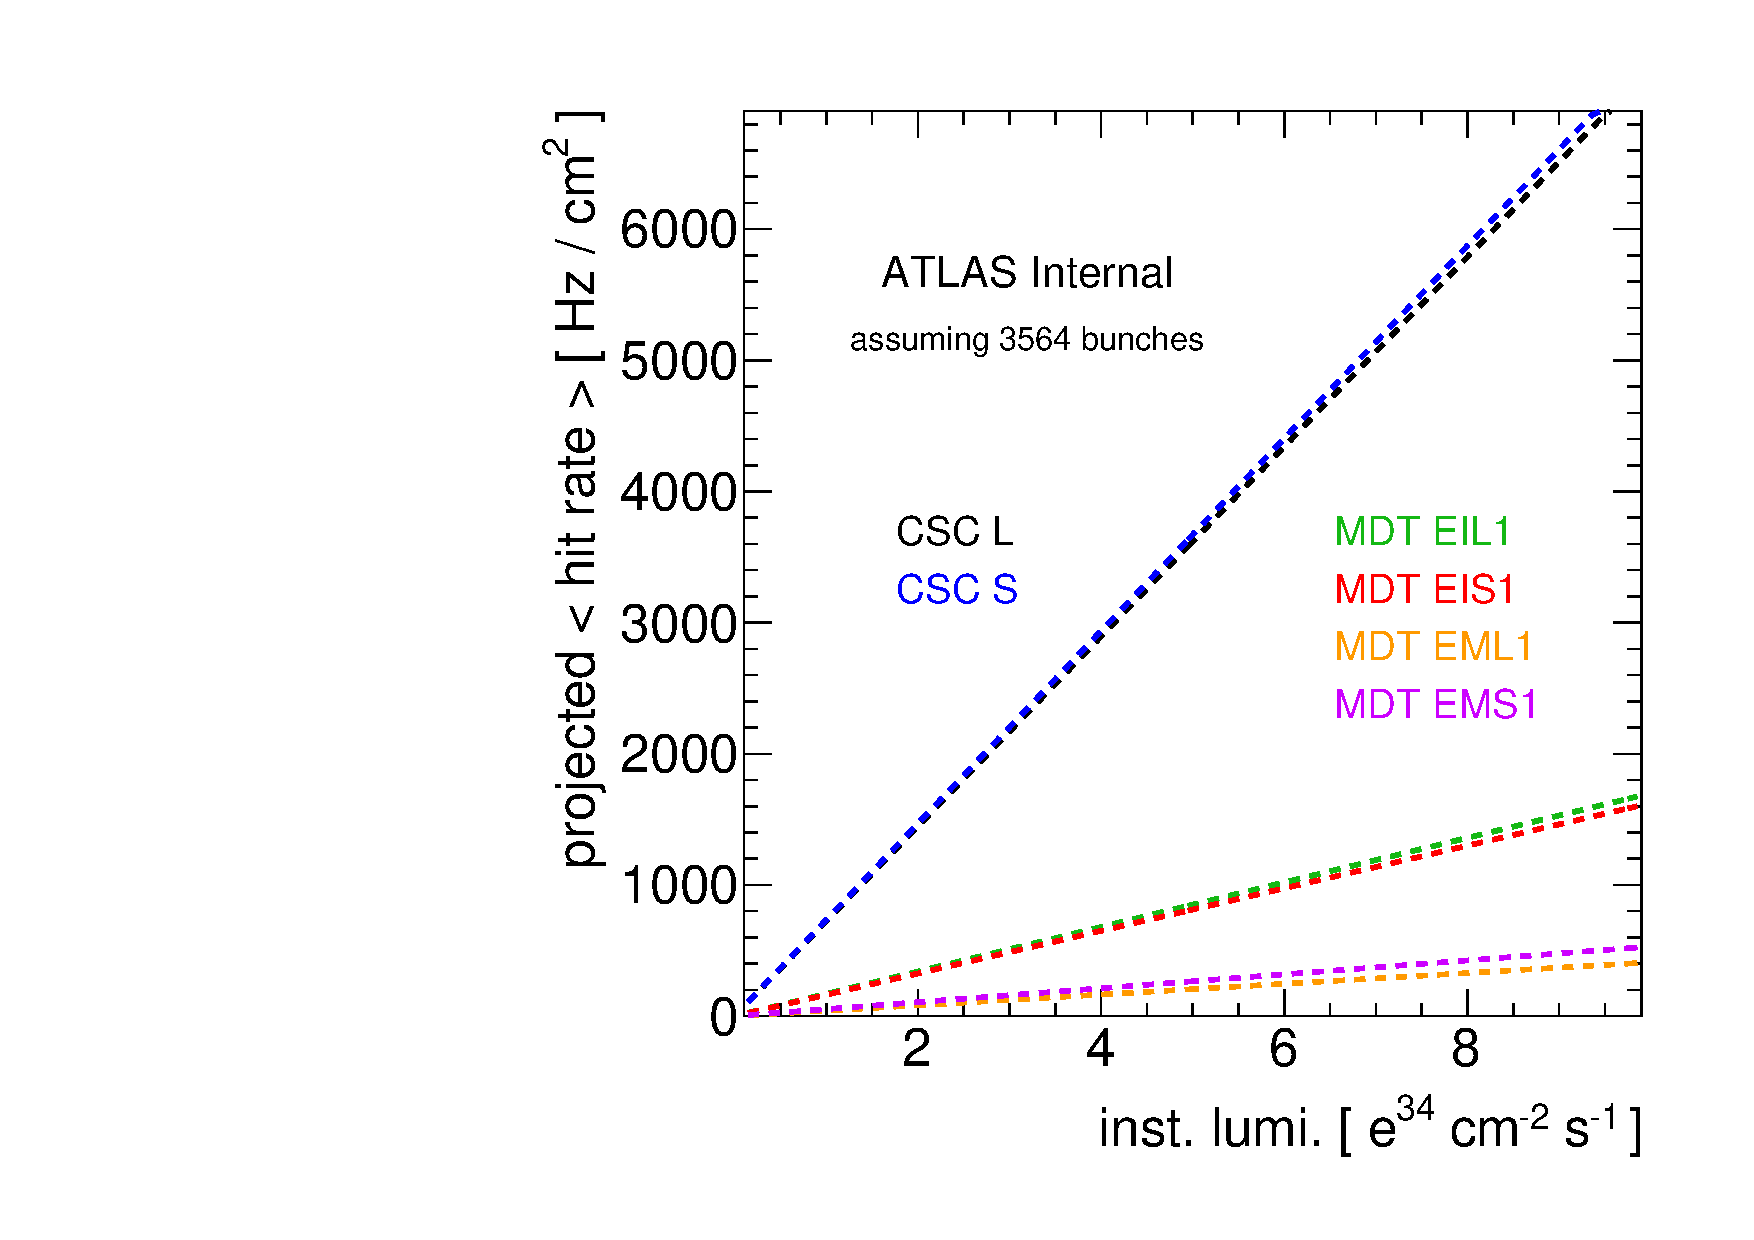
\includegraphics[width=0.45\textwidth]{./figures/extrapolate_vs_lumi_raw_3564.pdf}
    \caption{Projected inclusive hit rates in the MS as a function of instantaneous luminosity, assuming 2808 (left) and 3564 (right) filled bunches in the LHC. The CSC and MDT EI regions are overlaid.}
    \label{fig:extrapolations-hitrates-raw}
  \end{center}
\end{figure}

The projected average hit rates at Run 3 and HL-LHC conditions are shown in Table~\ref{tab:extrapolations-hitrates}, both inclusively and with ADC cuts. The instantaneous luminosity is assumed to be $2\times10^{34}$ in Run 3 and $7\times10^{34}$ at the HL-LHC. 

\newcommand*{\hspfou}{\hspace*{0.4cm}}

\begin{table}
  \begin{center}
    \renewcommand{\arraystretch}{1.4}
    \begin{tabular}{c||c|c||c|c}
      \multicolumn{1}{c}{}   & \multicolumn{4}{c}{\rate} \\
      \multicolumn{1}{c}{}   & \multicolumn{2}{c}{inclusive}                  & \multicolumn{2}{c}{with ADC cut} \\
      \hspsix Region \hspsix & \hspsix Run 3 \hspsix & \hspfou HL-LHC \hspfou & \hspsix Run 3 \hspsix & \hspfou HL-LHC \hspfou \\
      \hline\hline
      CSC L                  & 1598                  &  5065                  & 1093                  & 3338 \\
      CSC S                  & 1609                  &  5095                  & 1094                  & 3342 \\
      \hline
      MDT EIL1               &  377                  &  1189                  &  321                  & 1007 \\
      MDT EIS1               &  356                  &  1137                  &  304                  &  968 \\
      \hline
      MDT EML1               &   92                  &   287                  &   77                  &  241 \\
      MDT EMS1               &  120                  &   372                  &  100                  &  309 \\
      \hline\hline
      NSW, hottest           & 3560                  & 11200                  & 2420                  & 7390 \\
    \end{tabular}
    \caption{Projected hit rates at Run 3 and HL-LHC conditions in the hottest regions of the MS, both inclusively and with ADC cuts. Run 3 conditions assume $\mathcal{L}=2\times10^{34}$ and 2808 filled bunches in the LHC. HL-LHC conditions assume $\mathcal{L}=7\times10^{34}$ and 3564 filled bunches.}
    \label{tab:extrapolations-hitrates}
  \end{center}
\end{table}

The CSC hit rate in 2015 data-taking closest to the beampipe is at most $\sim\!2.2$ times larger than the average hit rate of the chamber, as discussed in Section~\ref{sec:hitrates}. This implies the hottest region of the small wheel at HL-LHC conditions will have a hit rate of 11.2 $\text{kHz} / \text{cm}^2$ when hits in 2015 data-taking are considered inclusively. The corresponding hit rate is 7.4 $\text{kHz} / \text{cm}^2$ when hits are considered with ADC cuts. These projections assume no changes in the ATLAS shielding or beam pipe.

The extrapolations here are generally consistent with previous extrapolations using the Run 1 dataset \cite{CERN-LHCC-2013-006,ATL-COM-MUON-2013-003,ATL-COM-MUON-2013-011}. The regions of the CSC closest to the beam pipe project to have a rate which is within the benchmark of 15 $\text{kHz} / \text{cm}^2$ considered in the NSW technical design report. Projections of the MDT hit rates are about 20\% lower than the Run 1 projections, which is expected from simulation, given the updates to the ATLAS beam pipe and shielding during Long Shutdown 1 \cite{ATL-COM-MUON-2014-027}.

\section{Conclusions}
\label{sec:conclusions}

This note presents measurements of the hit rates in the MDTs and CSCs of the ATLAS Muon Spectrometer in 2015 operation. The hit rates are considered as a function of detector region, instantaneous luminosity, and transverse distance from the beampipe. The hit rates show linear behavior as a function of the instantaneous luminosity, indicating good performance.

Additionally, the hit rates are projected to future data-taking conditions by extrapolating the linear behavior to the expected conditions in Run 3 and the HL-LHC. These runs are expected to operate with more filled bunches and higher instantaneous luminosity than are reached in 2015 operation. The maximum projected hit rate in the small wheel at HL-LHC conditions is 11.2 (7.4) $\text{kHz} / \text{cm}^2$ when hits are measured inclusively (with ADC cut). This projection does not consider future changes to the ATLAS shielding or beam pipe.



\section*{Acknowledgements}
%% Acknowledgements for papers with collision data
% Version 19-Feb-2015

% Standard acknowledgements start here
%----------------------------------------------
We thank CERN for the very successful operation of the LHC, as well as the
support staff from our institutions without whom ATLAS could not be
operated efficiently.

We acknowledge the support of ANPCyT, Argentina; YerPhI, Armenia; ARC,
Australia; BMWFW and FWF, Austria; ANAS, Azerbaijan; SSTC, Belarus; CNPq and FAPESP,
Brazil; NSERC, NRC and CFI, Canada; CERN; CONICYT, Chile; CAS, MOST and NSFC,
China; COLCIENCIAS, Colombia; MSMT CR, MPO CR and VSC CR, Czech Republic;
DNRF, DNSRC and Lundbeck Foundation, Denmark; EPLANET, ERC and NSRF, European Union;
IN2P3-CNRS, CEA-DSM/IRFU, France; GNSF, Georgia; BMBF, DFG, HGF, MPG and AvH
Foundation, Germany; GSRT and NSRF, Greece; RGC, Hong Kong SAR, China; ISF, MINERVA, GIF, I-CORE and Benoziyo Center, Israel; INFN, Italy; MEXT and JSPS, Japan; CNRST, Morocco; FOM and NWO, Netherlands; BRF and RCN, Norway; MNiSW and NCN, Poland; GRICES and FCT, Portugal; MNE/IFA, Romania; MES of Russia and ROSATOM, Russian Federation; JINR; MSTD,
Serbia; MSSR, Slovakia; ARRS and MIZ\v{S}, Slovenia; DST/NRF, South Africa;
MINECO, Spain; SRC and Wallenberg Foundation, Sweden; SER, SNSF and Cantons of
Bern and Geneva, Switzerland; NSC, Taiwan; TAEK, Turkey; STFC, the Royal
Society and Leverhulme Trust, United Kingdom; DOE and NSF, United States of
America.

The crucial computing support from all WLCG partners is acknowledged
gratefully, in particular from CERN and the ATLAS Tier-1 facilities at
TRIUMF (Canada), NDGF (Denmark, Norway, Sweden), CC-IN2P3 (France),
KIT/GridKA (Germany), INFN-CNAF (Italy), NL-T1 (Netherlands), PIC (Spain),
ASGC (Taiwan), RAL (UK) and BNL (USA) and in the Tier-2 facilities
worldwide.
%----------------------------------------------



\clearpage

\appendix
\part*{Appendix}
\addcontentsline{toc}{part}{Appendix}

\section{Details of the ZeroBias dataset}
\label{sec:zerobias}

Data events are collected via the \texttt{ZeroBias} stream. This stream replaces the \texttt{MinBias} stream in 2015 data-taking as the recommended source of unbiased proton collisions. Another usage of the stream is to provide data events used in MC overlay of additional pileup interactions. 

The stream triggers on ``zero bias'' events by acknowledging a L1 \texttt{EM15} trigger and recording the event one LHC orbit after this. This ensures the recorded event is from a filled bunch crossing but makes no further requirements of the event.

The stream is pre-scaled to 10 Hz throughout 2015. 5 Hz of triggers are allocated for inclusive zero bias events, \texttt{HLT\_noalg\_zb\_L1ZB}, and 5 Hz of triggers are allocated for zero bias events where additionally a jet is required at HLT with $\pt > 40$ GeV, \texttt{HLT\_j40\_L1ZB}. Both triggers are seeded by \texttt{L1\_ZB}. More details on the stream are available at the \href{https://twiki.cern.ch/twiki/bin/viewauth/Atlas/Run2StreamingSetup}{Run2StreamingSetup twiki}.

Data events are required to be in lumi blocks where all detector and reconstruction elements are reported to be functioning properly, which are collected in a good runs list (GRL). Exceptionally, Run 281143 is included in the GRL, when the insertable $b$-layer (IBL) was turned off. The absence of the IBL does not affect the \texttt{ZeroBias} triggers or the operation of the MDT and CSC. The GRL used here is:

\texttt{data15\_13TeV.periodAllYear\_DetStatus-v73-pro19-08\_DQDefects-00-01-02} \\
\texttt{\_PHYS\_StandardGRL\_All\_Good\_25ns\_tolerable\_IBLSTANDBY-DISABLE.xml}

Because the study is not statistically limited, not all events are used in the study. A random sample of 10-50\% of each run is used in the studies. The runs are described in more detail in Table~\ref{tab:zerobias}.

\begin{table}
  \begin{center}
    \begin{tabular}{c|c|c|c}
      Run    & Int. lumi. [\ipb] & Bunches & Events used \\
      \hline
      278880 &             22.7  &     447 & 51304 \\
      279169 &             57.8  &     733 & 70949 \\
      279345 &             54.9  &     877 & 53972 \\
      279685 &             78.2  &    1021 & 57115 \\
      280231 &             93.2  &    1165 & 51597 \\
      280464 &             61.5  &    1309 & 36492 \\
      280673 &            156.8  &    1453 & 33852 \\
      280862 &            137.8  &    1453 & 59833 \\
      281074 &             48.0  &    1596 & 36431 \\
      281143 &            210.2  &    1596 & 77801 \\
      281411 &            141.7  &    1813 & 46019 \\
      282992 &            112.1  &    1813 & 63457 \\
      283429 &            243.0  &    2029 & 73039 \\
      283780 &            151.3  &    2232 & 73218 \\
      284213 &            207.7  &    2232 & 77754 \\
      284285 &            255.8  &    2232 & 74323 \\
    \end{tabular}
    \caption{Data-taking conditions for runs used in the MDT/CSC hit rate studies. The integrated luminosity is taken from \href{https://atlas-lumicalc.cern.ch/results/b8e9b9/result.html}{lumicalc (b8e9b9)}.}
    \label{tab:zerobias}
  \end{center}
\end{table}



\section{Cleaning for emittance scans}
\label{sec:emittance}

During 2015 data-taking, the LHC sometimes performed short van der Meer scans during collisions to track the beam emittance. This led to rapidly changing instantaneous luminosity across only a few lumi blocks, as shown in Figure~\ref{fig:emittance-scans}. These lumi blocks are marked with tolerable DQ defects because the reported luminosity is unreliable.

\begin{figure}
  \begin{center}
    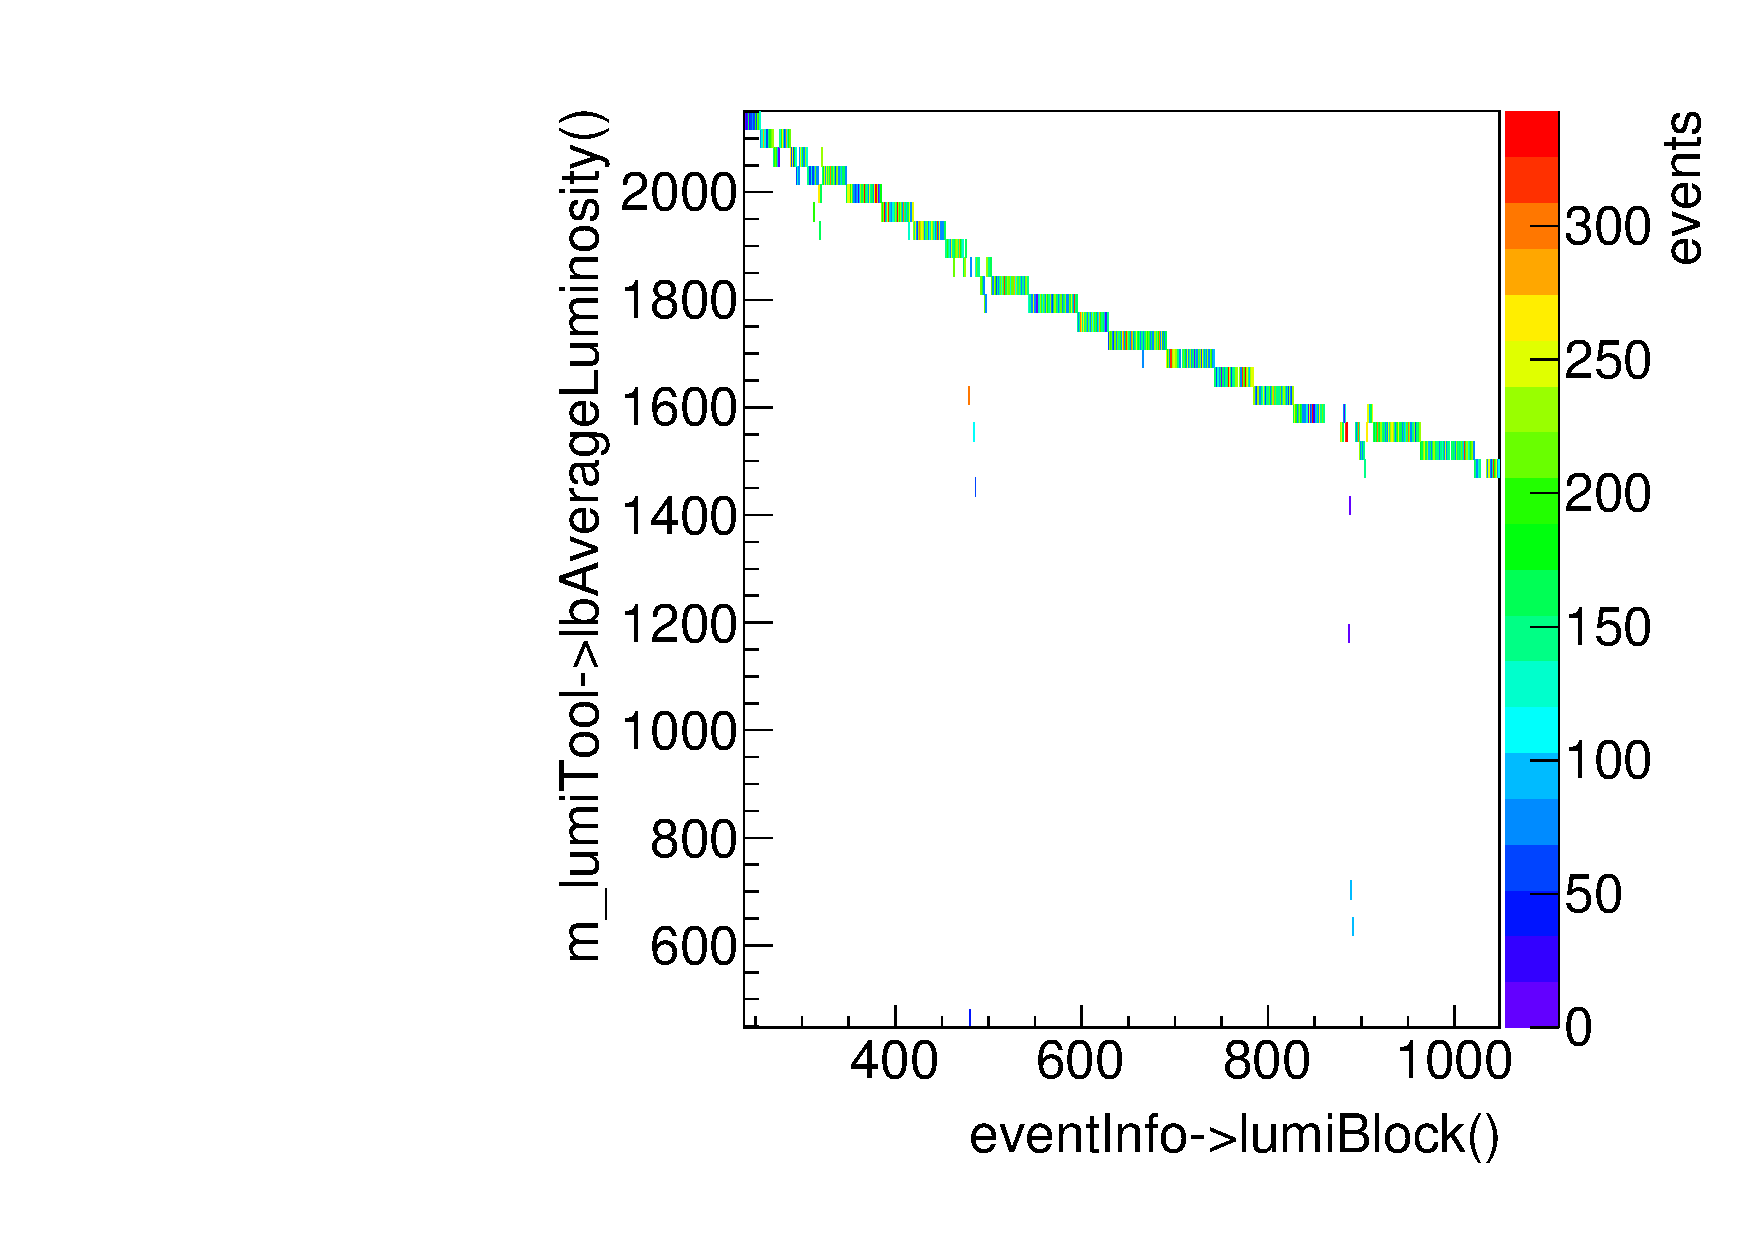
\includegraphics[width=0.45\textwidth]{./figures/lumi_vs_lb_00279685.pdf}
    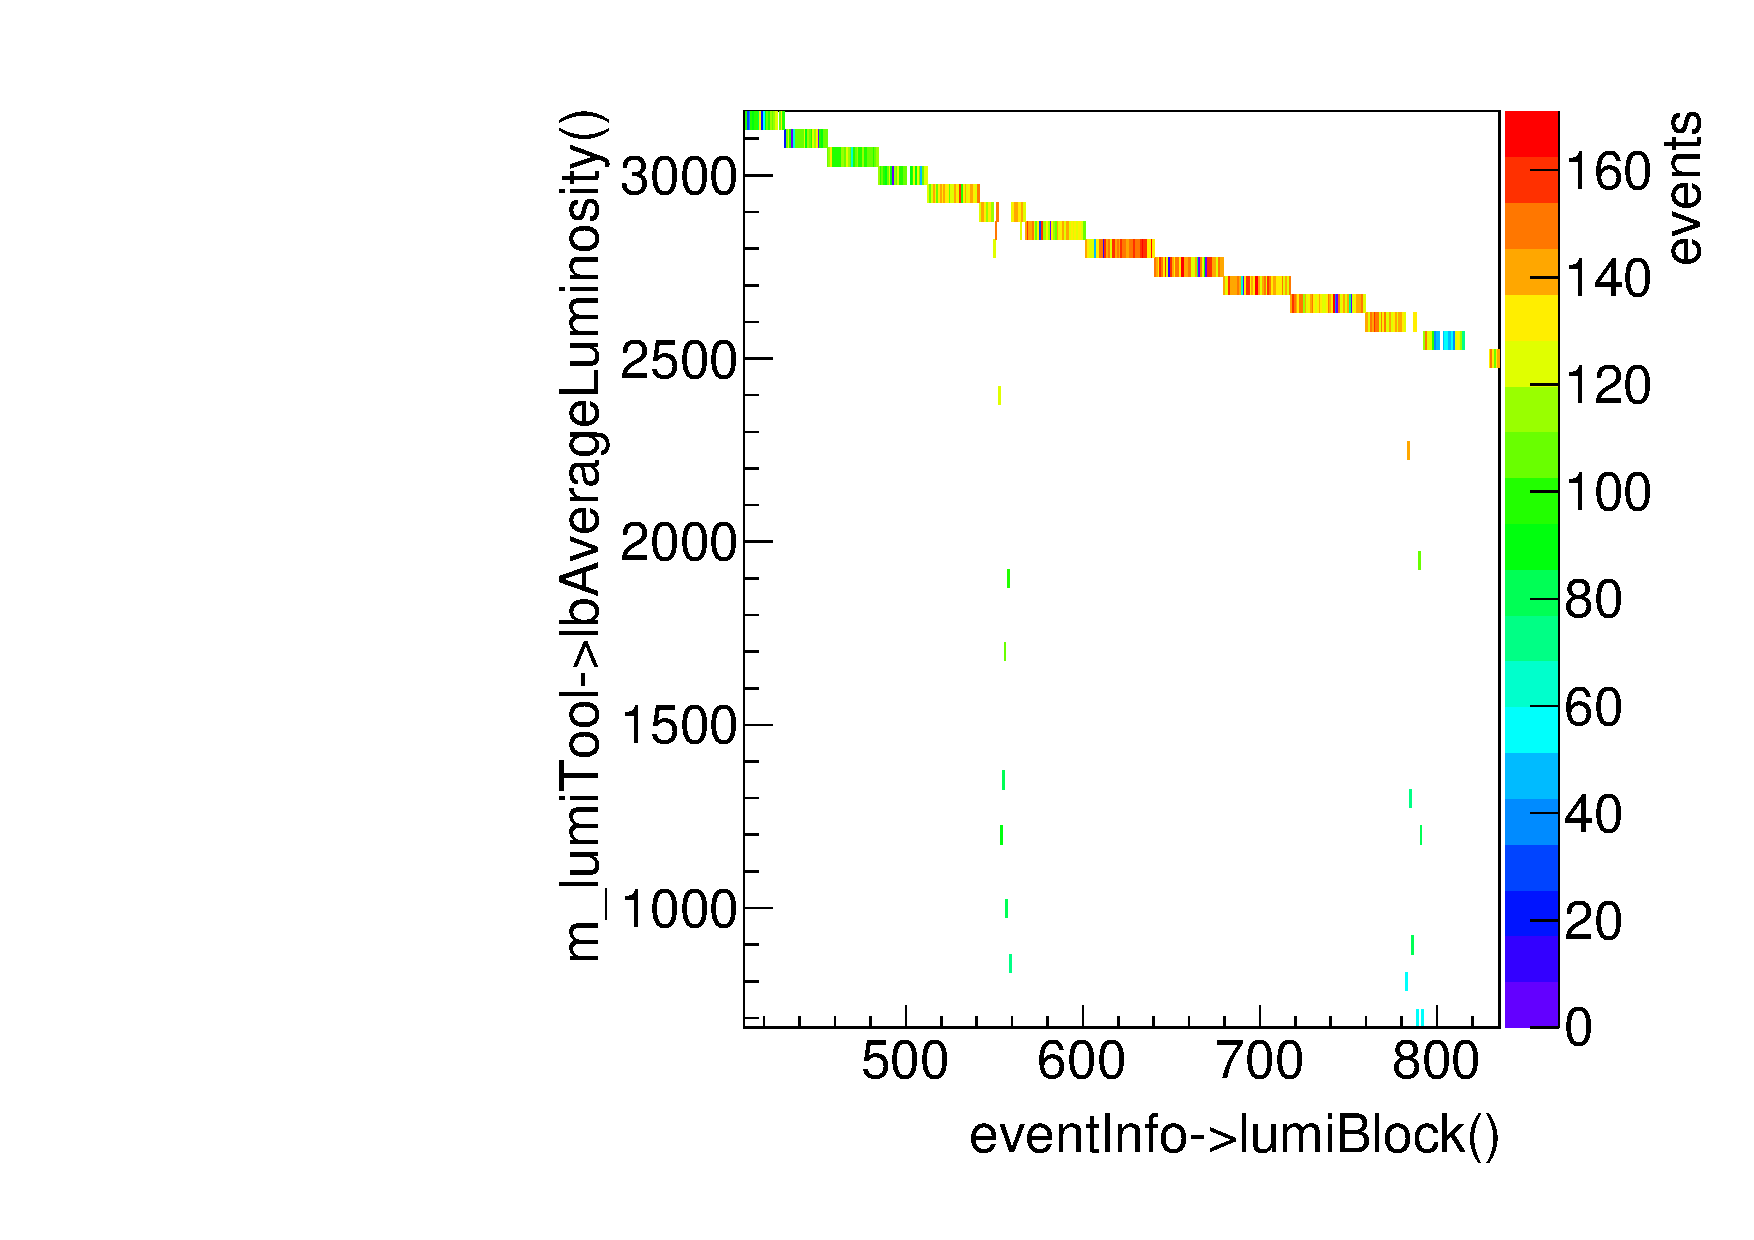
\includegraphics[width=0.45\textwidth]{./figures/lumi_vs_lb_00280464.pdf}
    \caption{Number of events in a given lumiblock and for a given instantaneous luminosity in Run 279685 (left) and 280464 (right). }
    \label{fig:emittance-scans}
  \end{center}
\end{figure}

The study of hit rates in the MDTs and CSCs depends heavily on the reported luminosity. Lumi blocks where the instantaneous luminosity is rapidly changing are therefore excluded from this study, as discussed in consultation with the \href{http://cern.ch/go/t7ND}{ATLAS Luminosity Group}.


\section{Removing noisy MDT tubes}
\label{sec:noisytubes}

The MDTs are composed of hundreds of thousands of drift tubes. A small fraction of these tubes show noisy behavior such that they record hits at a much higher rate than expected from incident particles. They are therefore discarded from this analysis to avoid biasing the measurements, both in counting hit tubes and in deriving the active area of the MDTs.

Noisy tubes are identified by observing the tube-level occupancy in Run 284285. As shown in Figure~\ref{fig:noisytubes}, the long tail at high occupancy indicates that a few tubes fire 1-2 orders of magnitude more often than most. Judging the spectrum by eye, tubes are marked as noisy if they fired in more than 10\% of events in Run 284285.

\begin{figure}
  \begin{center}
    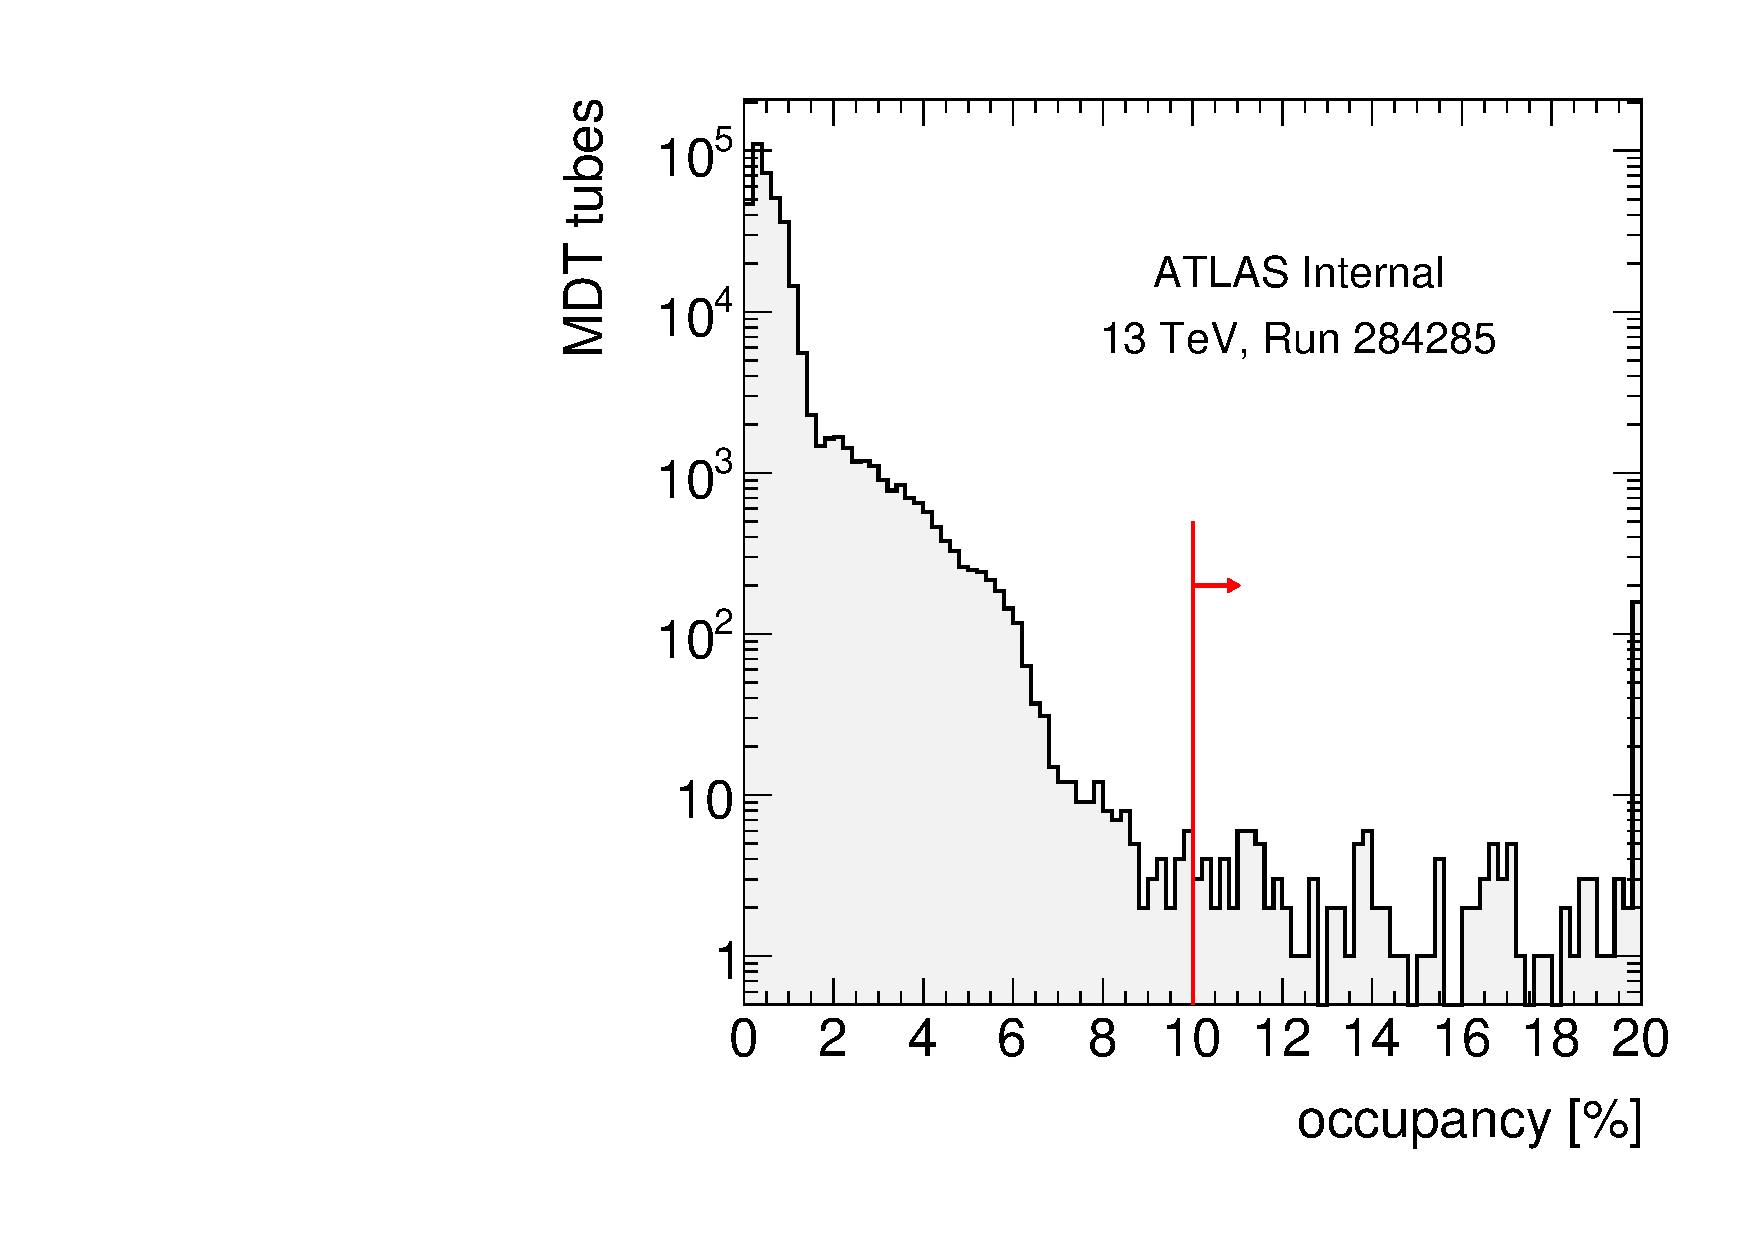
\includegraphics[width=0.45\textwidth]{./figures/occupancy_00284285.pdf}
    \caption{MDT tube occupancy in Run 284285. Most tubes fire in less than 2\% of events, but some fire at much larger rates. Tubes which fire in greater than 10\% of events in Run 284285 are considered noisy and discarded in this analysis.}
    \label{fig:noisytubes}
  \end{center}
\end{figure}



\section{Figures with ADC cuts}
\label{sec:electronicnoise}

The main body of the note describes a projection of CSC and MDT hit rates to future data-taking conditions, both inclusively and with ADC cuts applied to suppress electronic noise. However, only figures of inclusive hits are shown. This appendix presents the corresponding figures in the case of ADC cuts applied, as described in Table~\ref{tab:electronic-rawvsadc}.

% The hit rates presented in the main body of the note include all reported hits, including those from electronic noise. The contribution from electronic noise is detector-dependent, hence the inclusive hit rate is less useful for projecting to future LHC conditions because new detectors (sTGC, MM) will be deployed in the NSW. This appendix reports the hit rates with hit quality criteria cuts (\textit{ADC cuts}) which remove a large fraction of electronic noise while maintaining high efficiency for hits from incident particles. This is a more accurate reflection of the conditions for future MS detectors, though a proper unfolding to particle fluxes is still not attempted. The quality cuts considered for suppressing electronic noise are shown in Table~\ref{tab:electronic-adc}.

%% \begin{table}
%%   \begin{center}
%%     \begin{tabular}{c|c}
%%       detector & quality criteria \\
%%       \hline
%%       MDT      & tube ADC greater than 50 \\
%%       CSC      & maximum cluster strip ADC greater than 100 \\
%%     \end{tabular}
%%     \caption{Criteria for a MDT tube hit or CSC cluster passing noise thresholds.}
%%     \label{tab:electronic-adc}
%%   \end{center}
%% \end{table}

\begin{table}
  \begin{center}
    \renewcommand{\arraystretch}{1.4}
    \begin{tabular}{c|c|c}
      figure                              & inclusive                                     & quality criteria \\
      \hline
      hit rates per region                & Fig.~\ref{fig:hitrates-vs-region-raw}              & Fig.~\ref{fig:hitrates-vs-region-adc} \\
      CSC hit rates vs. inst. lumi.       & Fig.~\ref{fig:hitrates-vs-lumi-csc-raw}            & Fig.~\ref{fig:hitrates-vs-lumi-csc-adc} \\
      hit rates vs. $r$                   & Fig.~\ref{fig:hitrates-vs-r-raw}                   & Fig.~\ref{fig:hitrates-vs-r-adc} \\
      fitted slopes vs. N(bunches)        & Fig.~\ref{fig:extrapolations-slope-vs-bunches-raw} & Fig.~\ref{fig:extrapolations-slope-vs-bunches-adc} \\
      projected hit rates vs. inst. lumi. & Fig.~\ref{fig:extrapolations-hitrates-adc}         & Fig.~\ref{fig:extrapolations-hitrates-adc} \\
    \end{tabular}
    \caption{Figures reported the inclusive hit rates and their equivalent figures reported with quality criteria requirements.}
    \label{tab:electronic-rawvsadc}
  \end{center}
\end{table}

\begin{figure}
  \begin{center}
    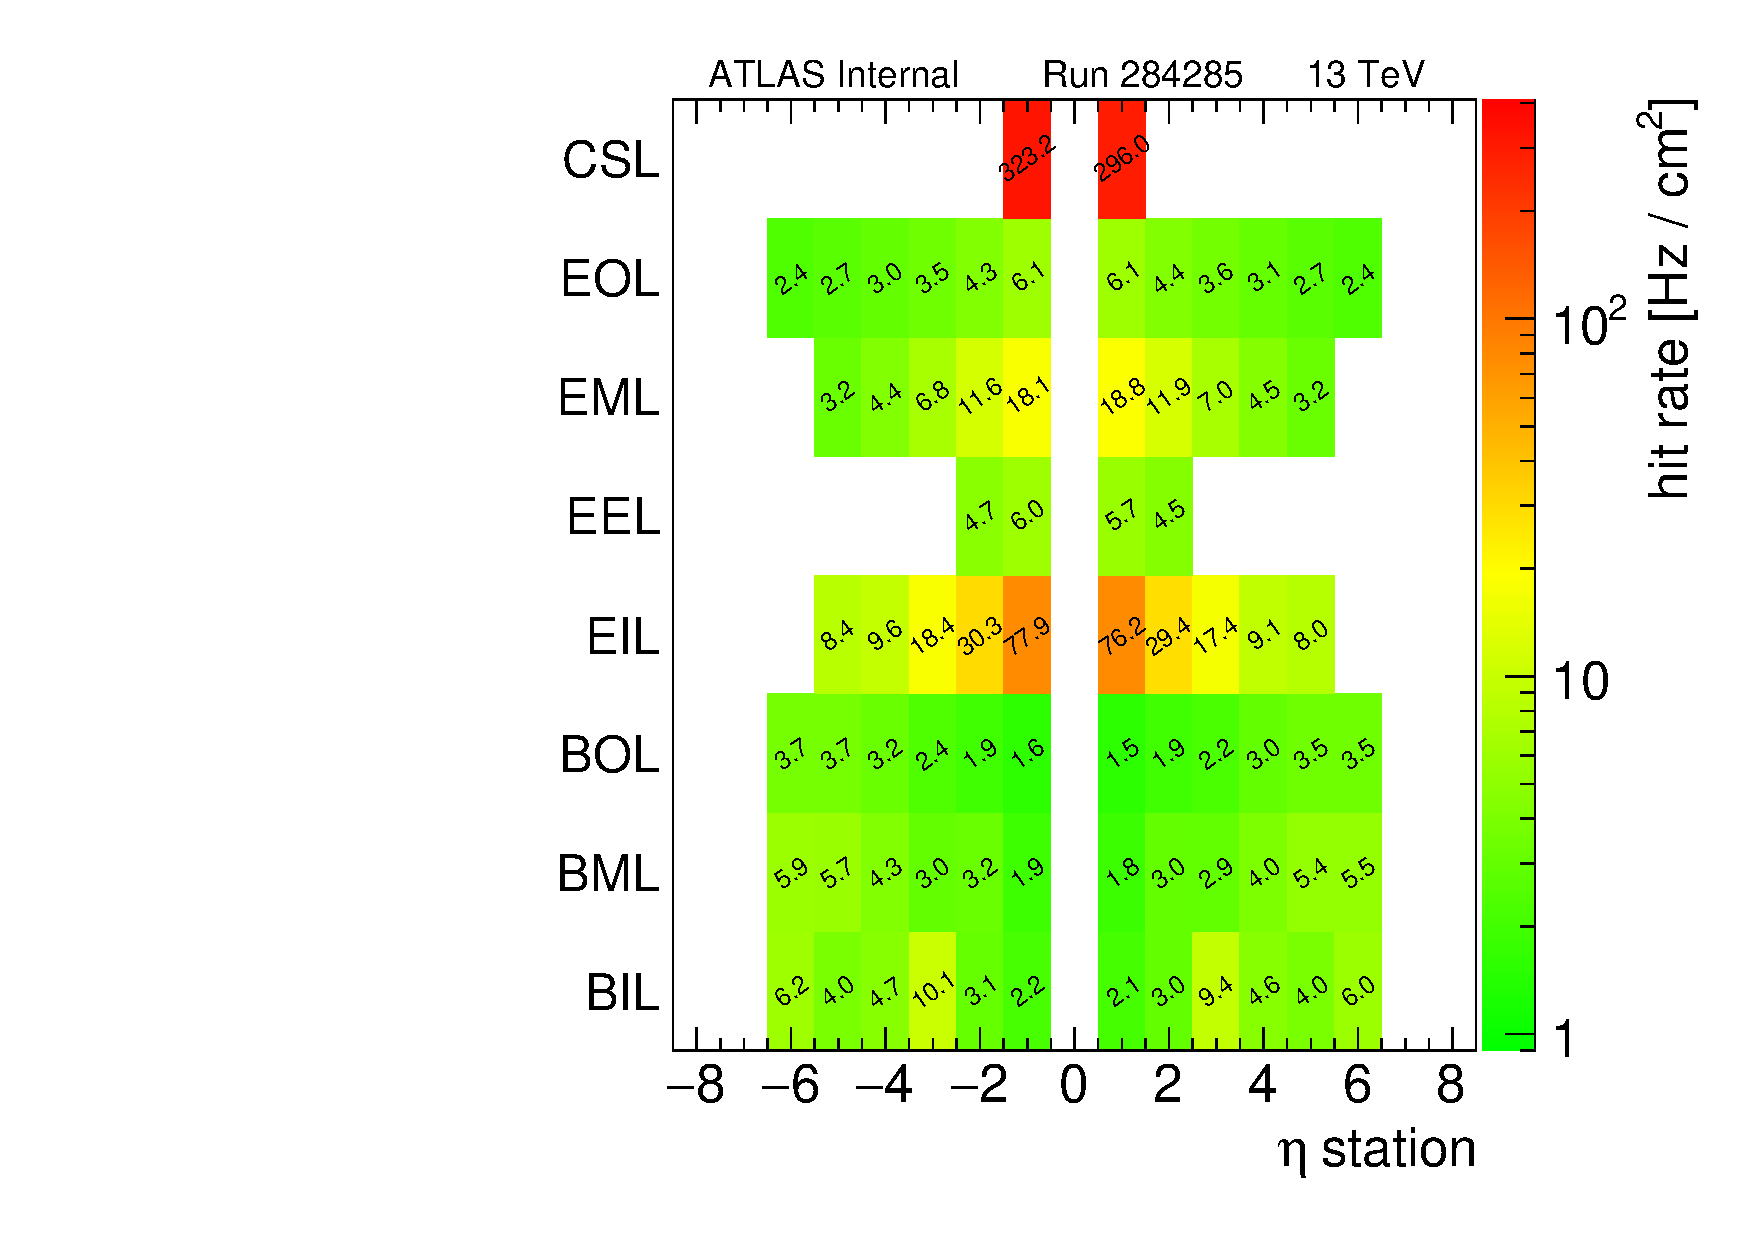
\includegraphics[width=0.45\textwidth]{./figures/rate_adc_vs_region_L_00284285.pdf}
    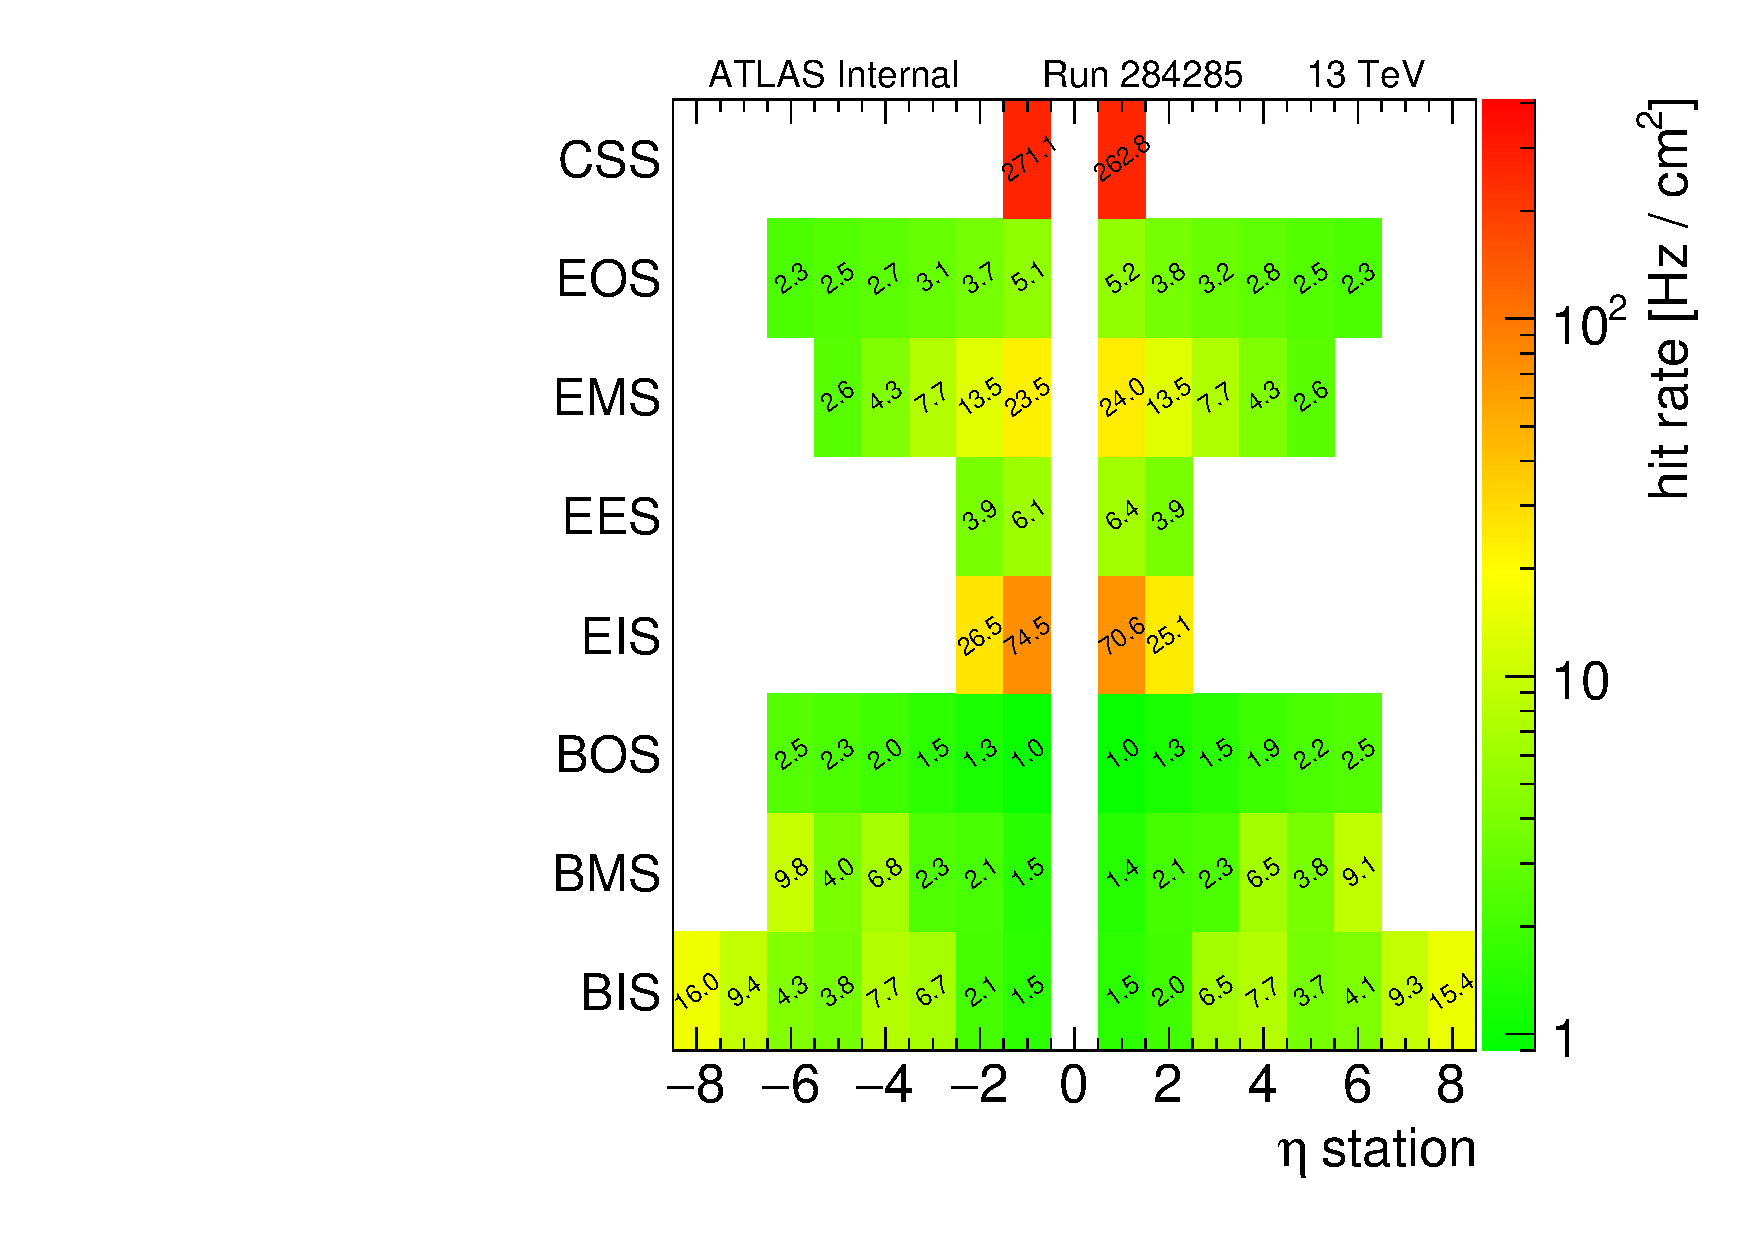
\includegraphics[width=0.45\textwidth]{./figures/rate_adc_vs_region_S_00284285.pdf}
    \caption{Total hit rate in the MDTs in Run 284285 in the largest regions of the detector. The rates are split into large sectors (left) and small sectors (right). Positive eta stations indicate the $+z$ side of ATLAS, and negative eta stations indicate the $-z$ side.}
    \label{fig:hitrates-vs-region-adc}
  \end{center}
\end{figure}

\begin{figure}
  \begin{center}
    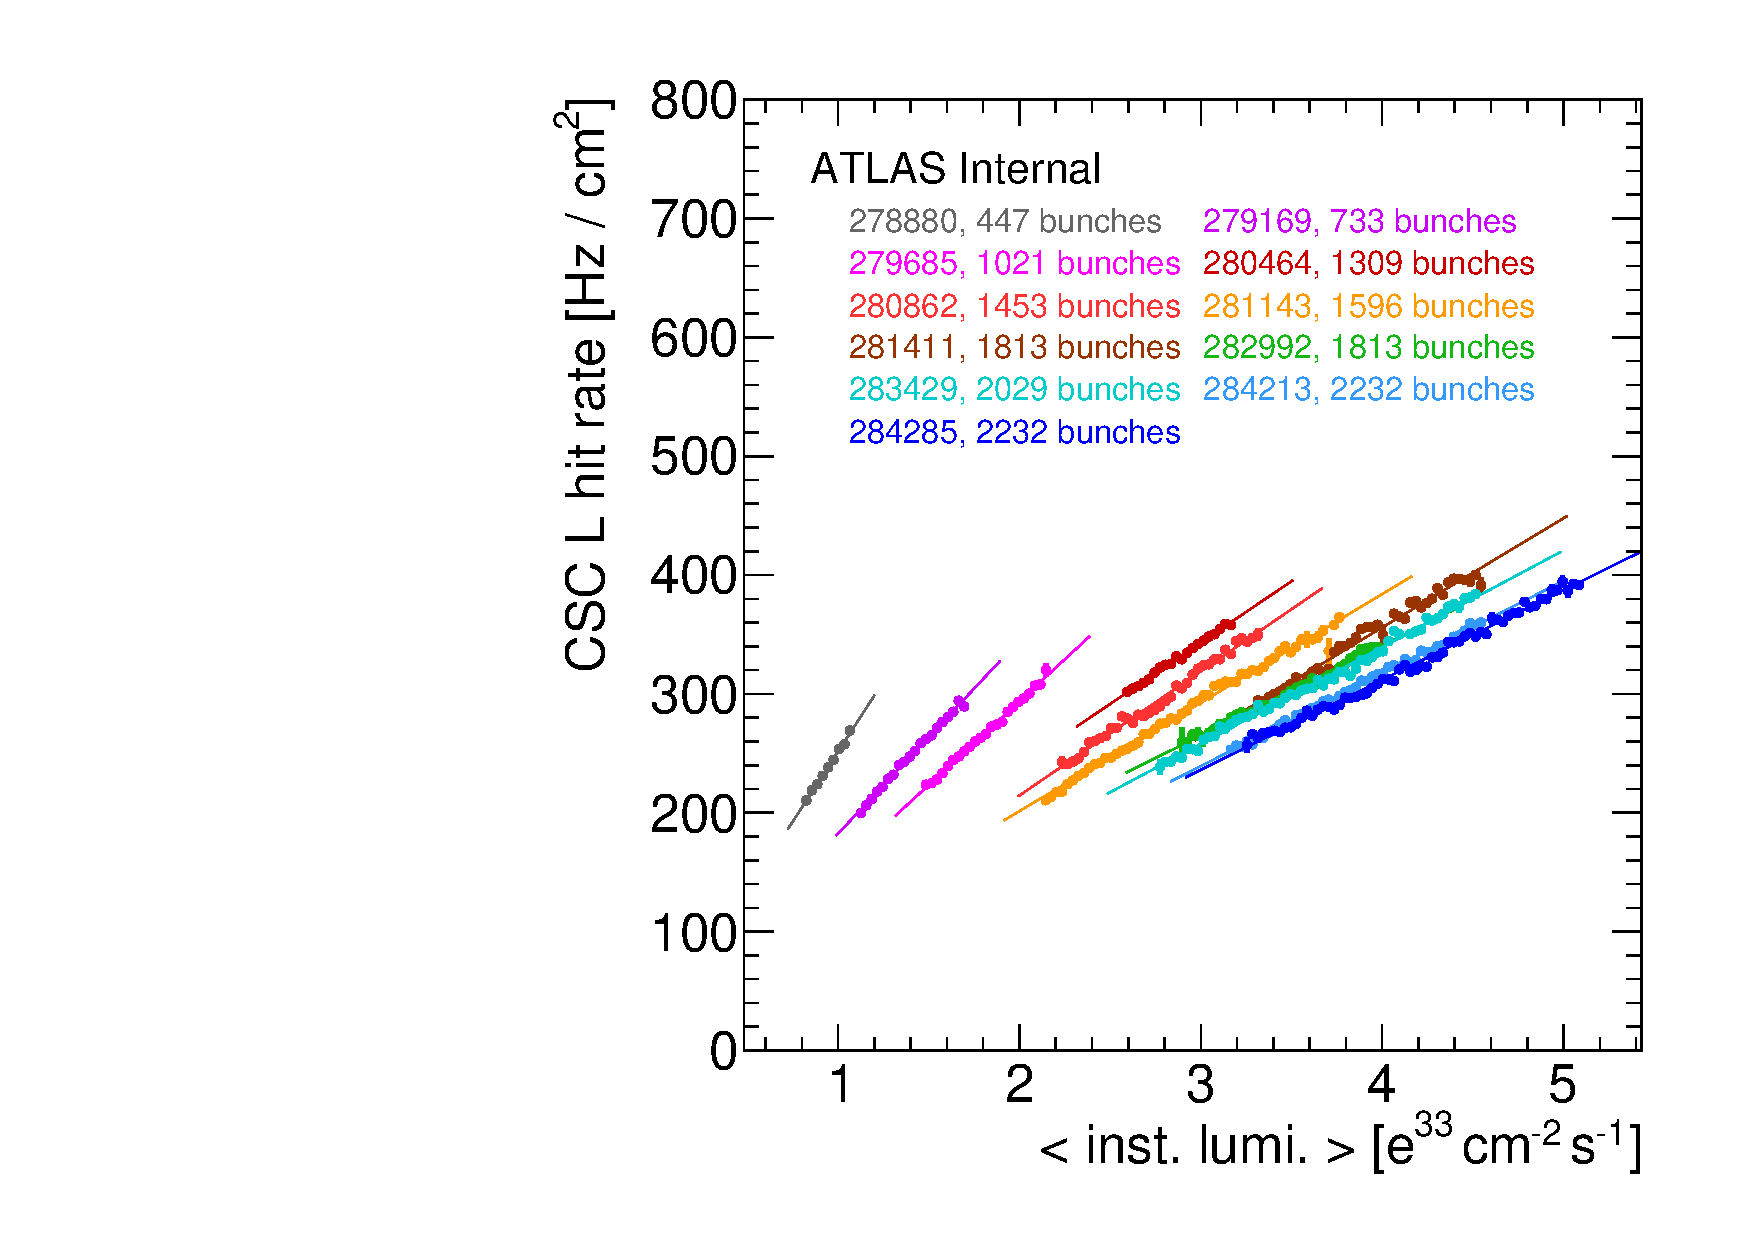
\includegraphics[width=0.45\textwidth]{./figures/rate_adc_vs_lumi_vs_evts_csc_CSL1_overlay.pdf}
    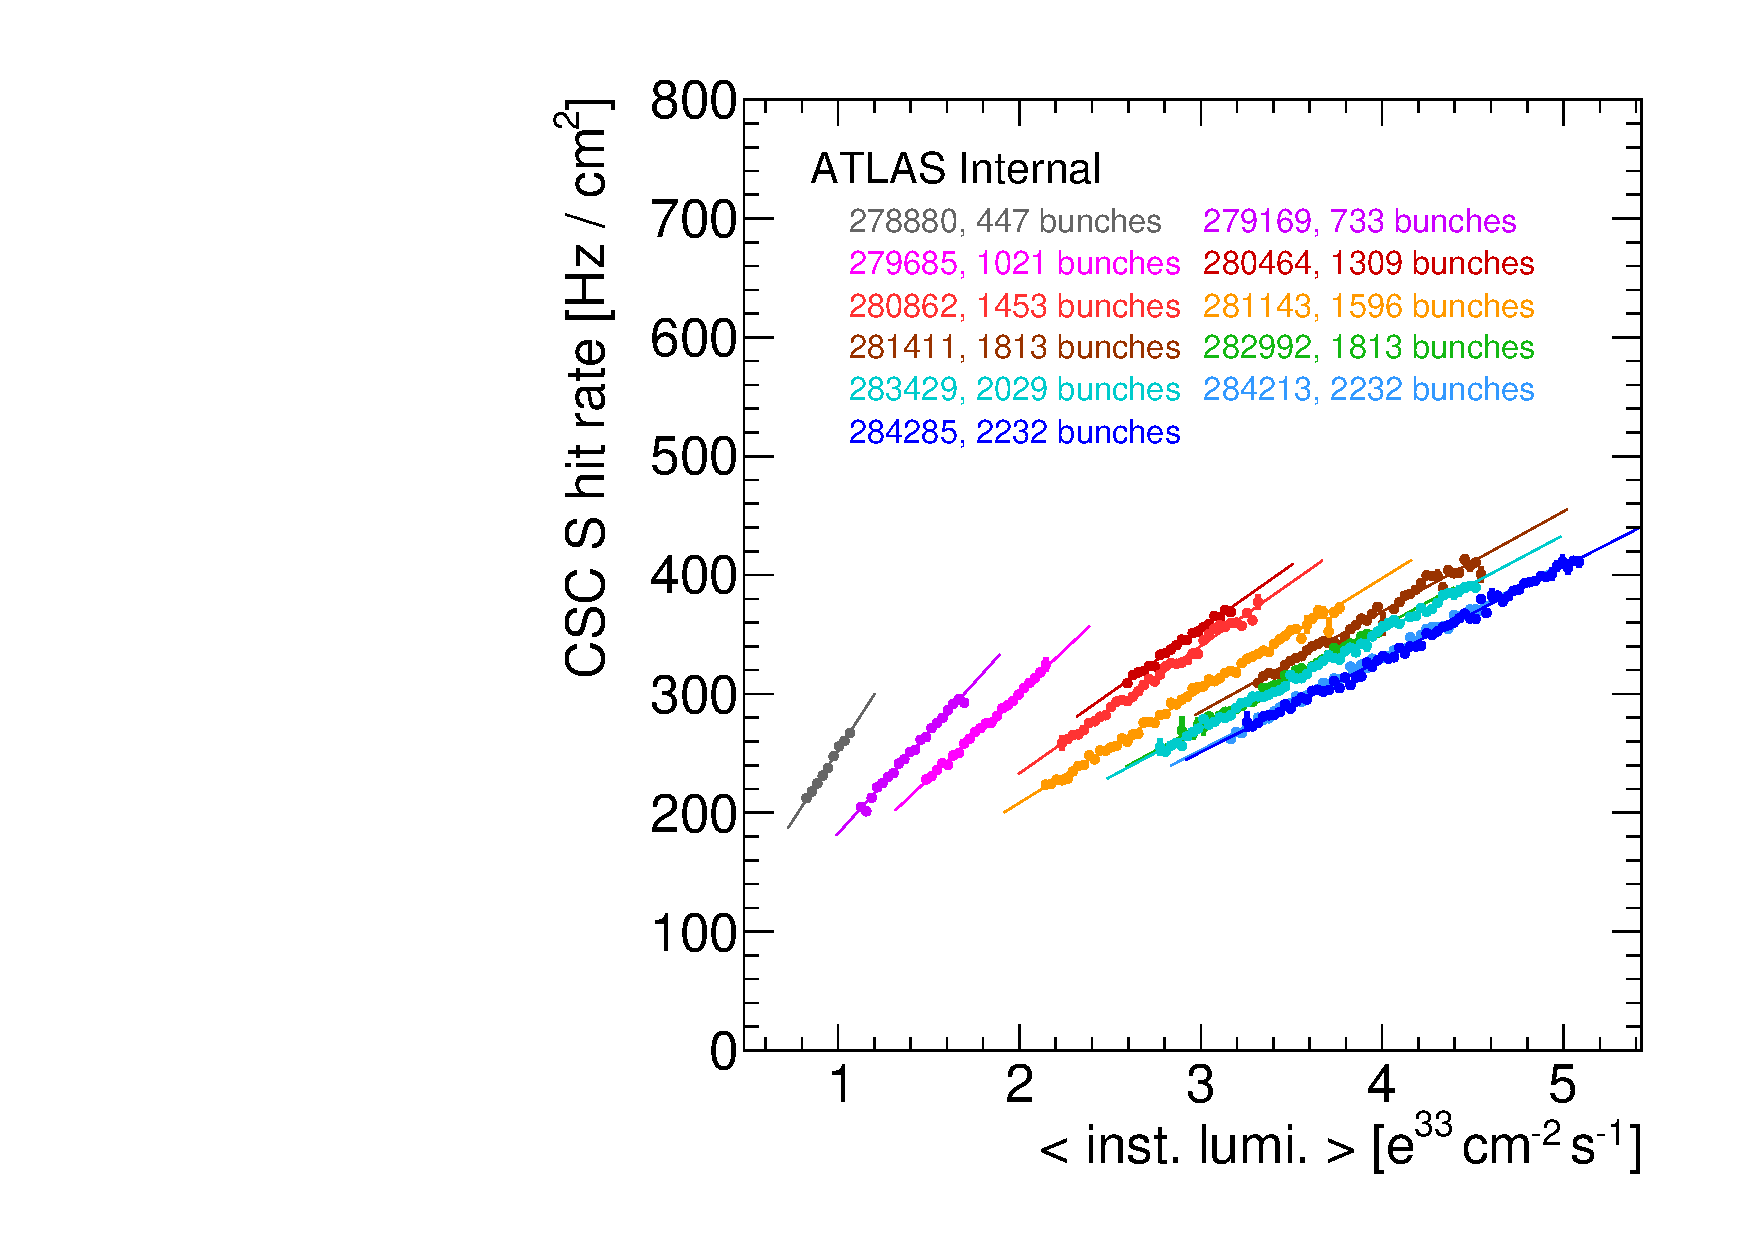
\includegraphics[width=0.45\textwidth]{./figures/rate_adc_vs_lumi_vs_evts_csc_CSS1_overlay.pdf}
    \caption{Total hit rate in the CSC large (left) and small (right) chambers as a function of instantaneous luminosity, for multiple runs.}
    \label{fig:hitrates-vs-lumi-csc-adc}
  \end{center}
\end{figure}

\begin{figure}
  \begin{center}
    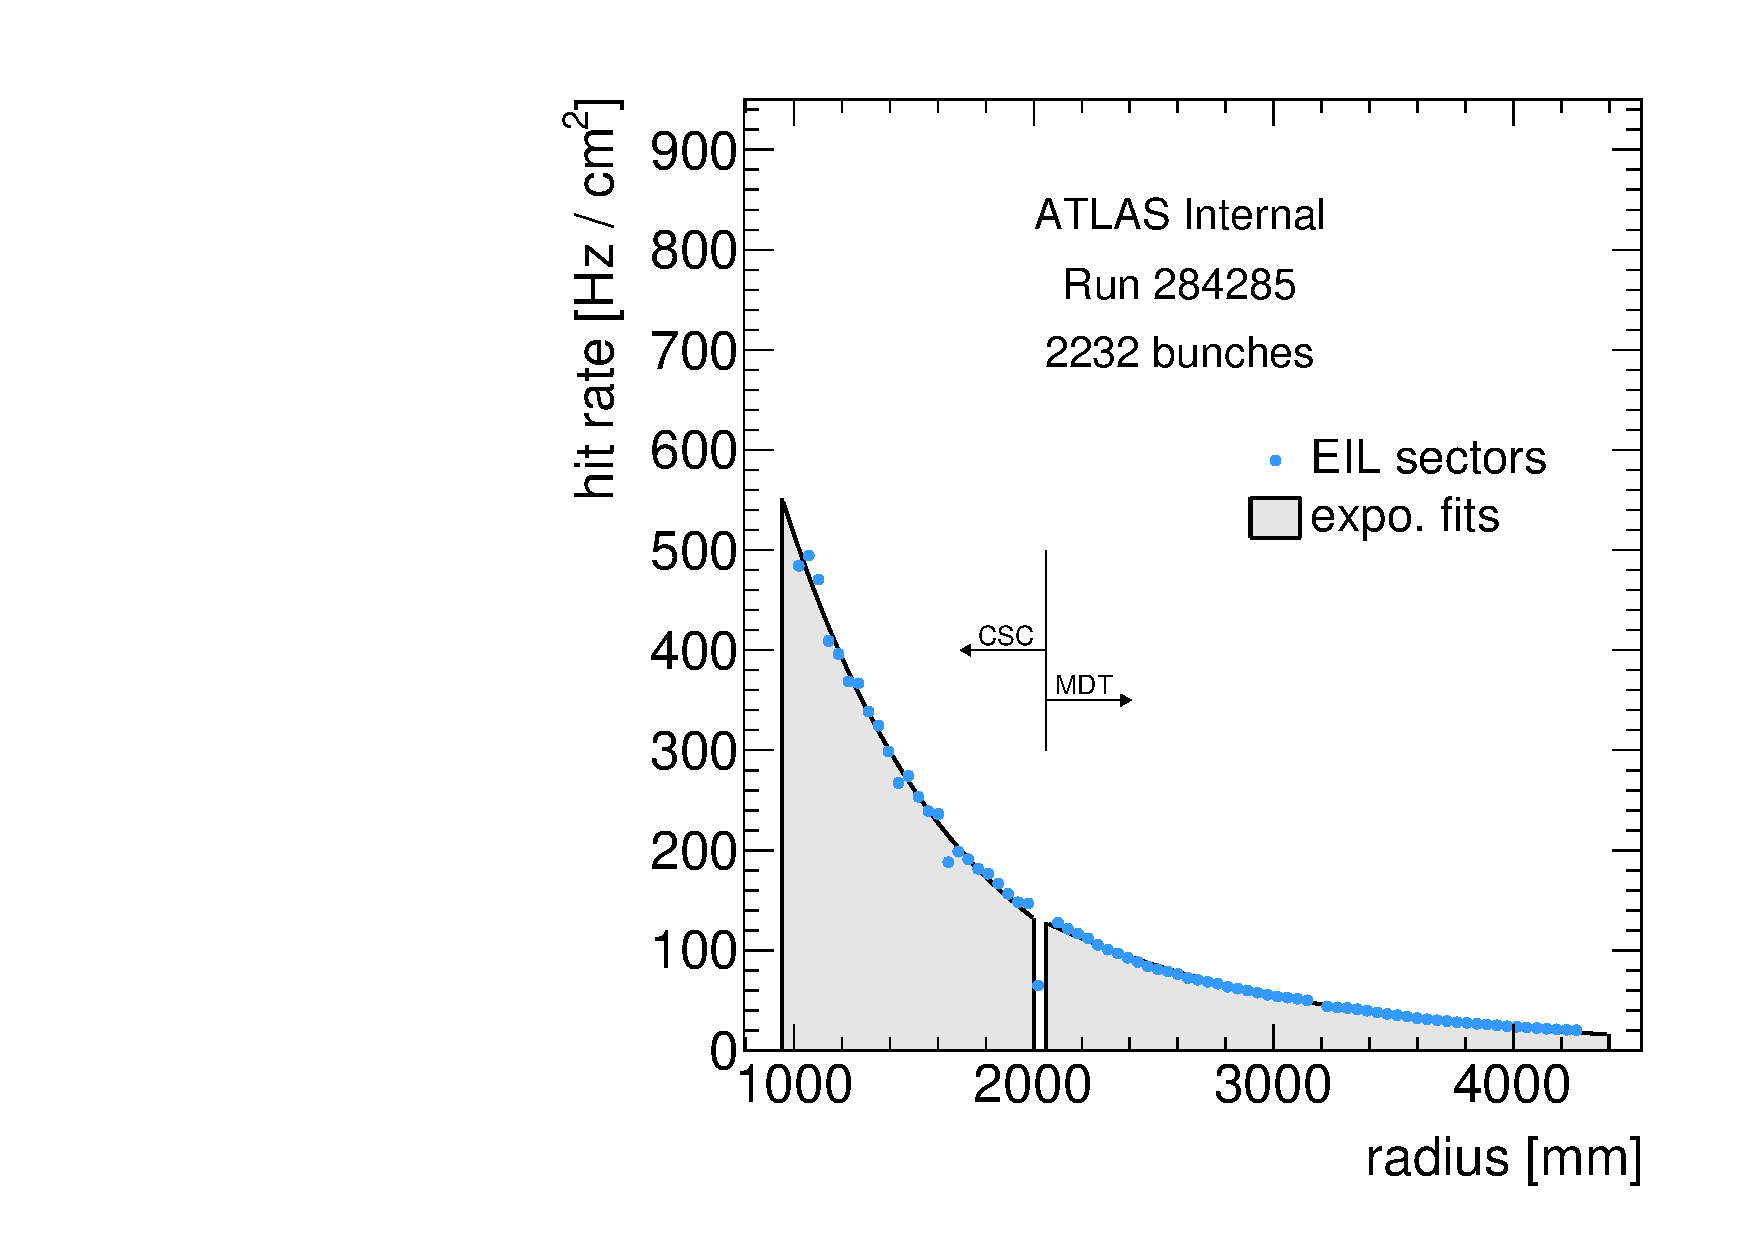
\includegraphics[width=0.45\textwidth]{./figures/rate_adc_vs_r_EIL_00284285.pdf}
    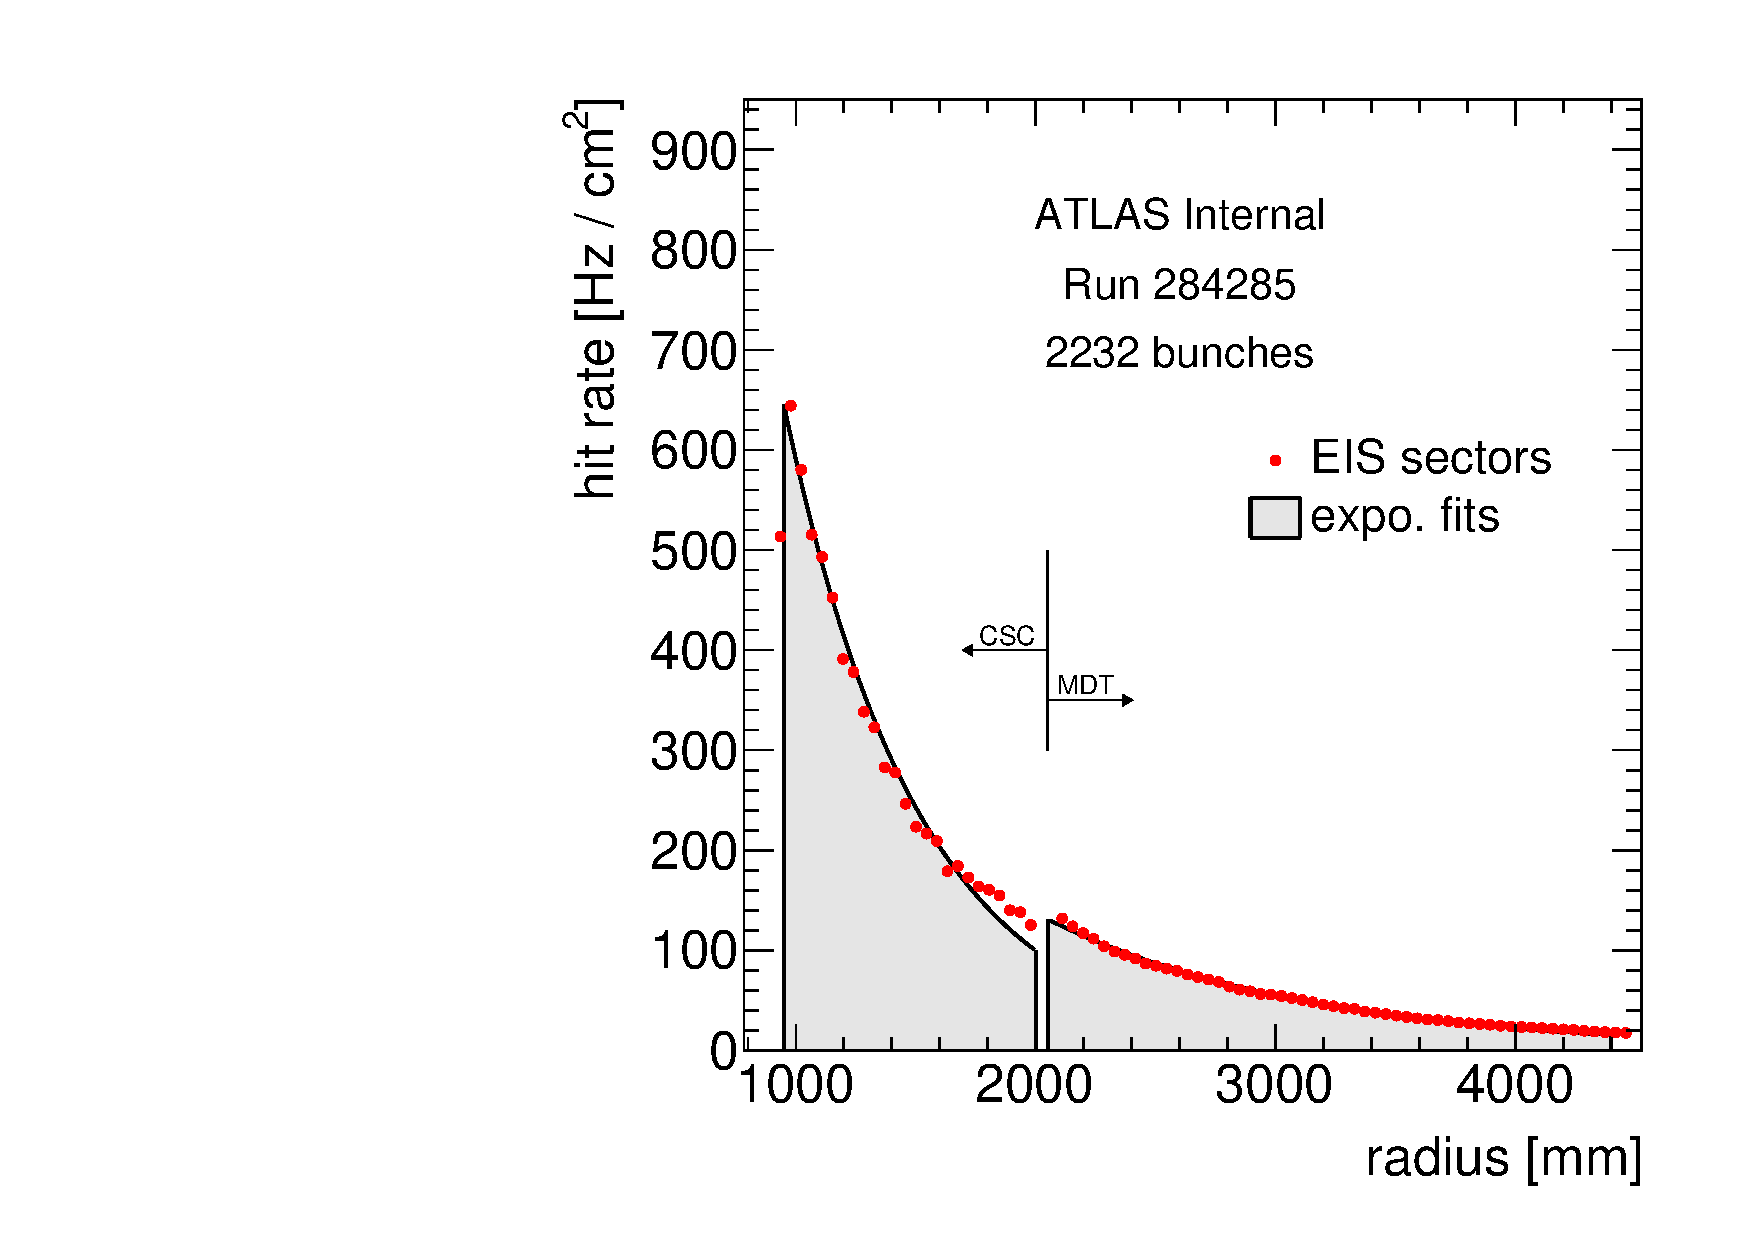
\includegraphics[width=0.45\textwidth]{./figures/rate_adc_vs_r_EIS_00284285.pdf}
    \caption{Total hit rate as a function of the transverse distance from the beam pipe in the small wheel, for large (left) and small (right) sectors, in Run 284285.}
    \label{fig:hitrates-vs-r-adc}
  \end{center}
\end{figure}

\begin{table}
  \begin{center}
    \renewcommand{\arraystretch}{1.4}
    \begin{tabular}{c|c|c|c}
      \multicolumn{1}{c|}{}              & \multicolumn{2}{c|}{\rate}                               & \multicolumn{1}{c}{} \\
      \hspace{0.6cm}region\hspace{0.6cm} & \hspace{0.6cm}average\hspace{0.6cm} & peak: smallest $r$ & peak / average \\
      \hline\hline
      % CSC L                              & 310                                 & 601                & 1.94 \\
      % CSC S                              & 324                                 & 738                & 2.28 \\
    \end{tabular}
    \caption{Comparison of the CSC chamber average hit rate with the hit rate closest to the beampipe in Run 284285. The average luminosity in Run 284285 is $\mathcal{L}=4.1\times10^{33}$.}
    \label{tab:hitrates-vs-r-adc}
  \end{center}
\end{table}

\begin{figure}
  \begin{center}
    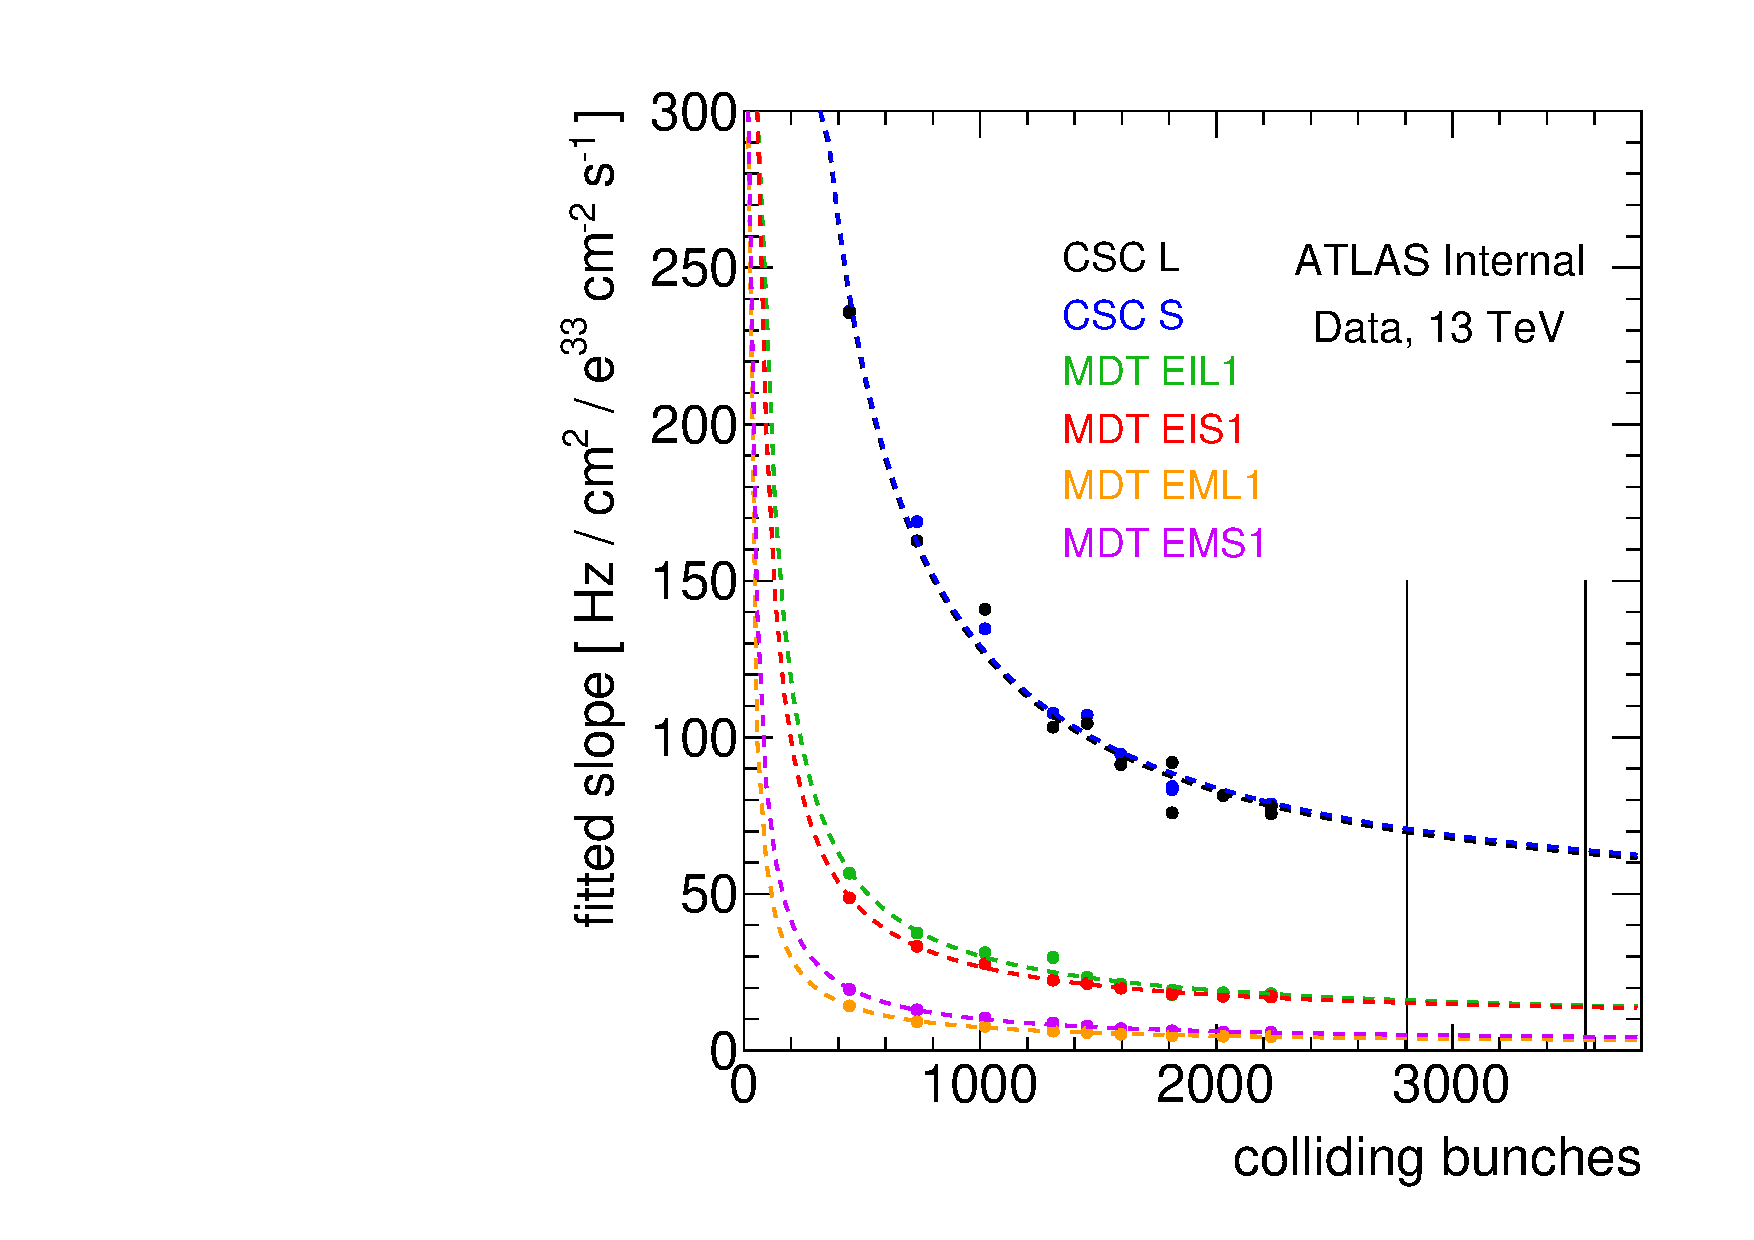
\includegraphics[width=0.45\textwidth]{./figures/slope_vs_bunches_adc_lin.pdf}
    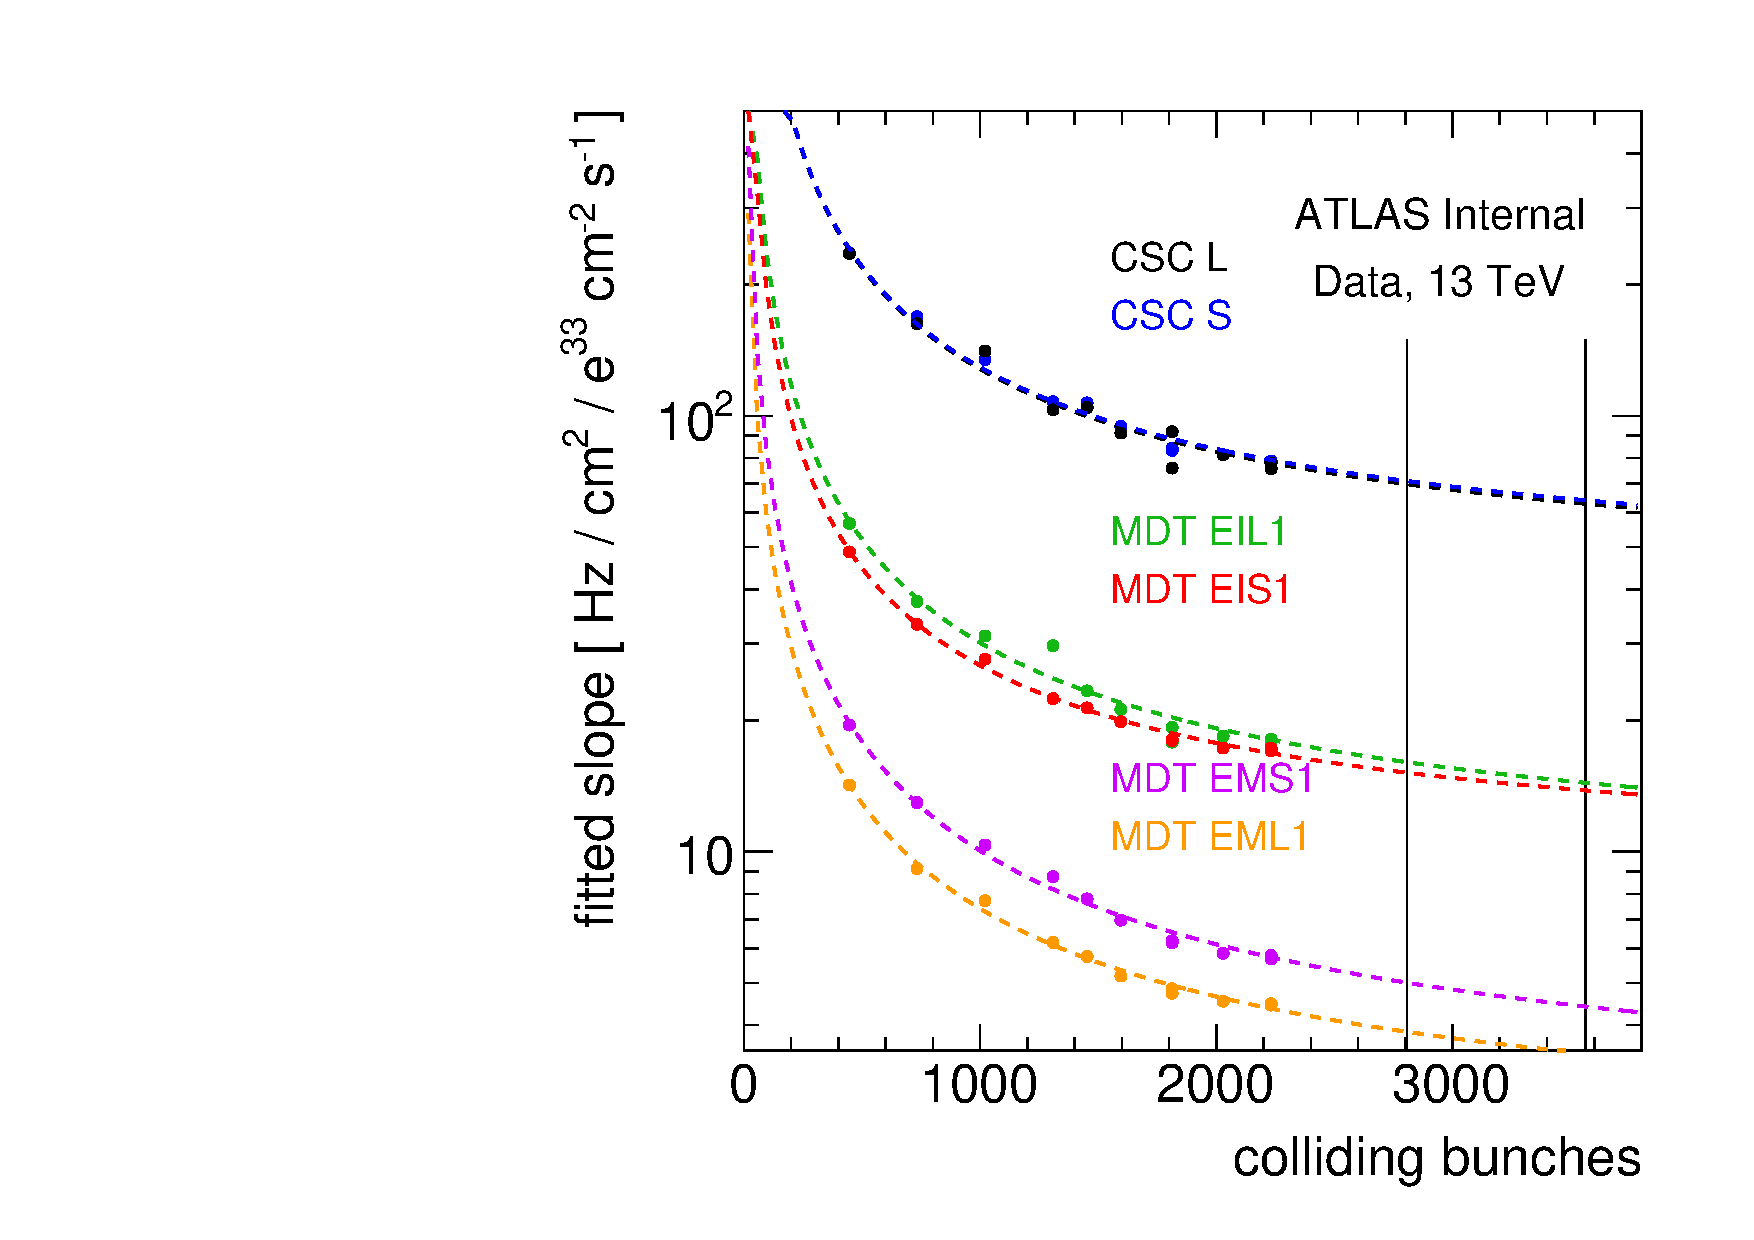
\includegraphics[width=0.45\textwidth]{./figures/slope_vs_bunches_adc_log.pdf}
    \caption{The fitted slope as a function of the number of colliding bunches for various runs in the hottest MDT and CSC chambers, shown with linear (left) and logarithmic (right) scale. The spectra are fitted to $A + B/x$, where $x$ is the number of bunches.}
    \label{fig:extrapolations-slope-vs-bunches-adc}
  \end{center}
\end{figure}

\begin{figure}
  \begin{center}
    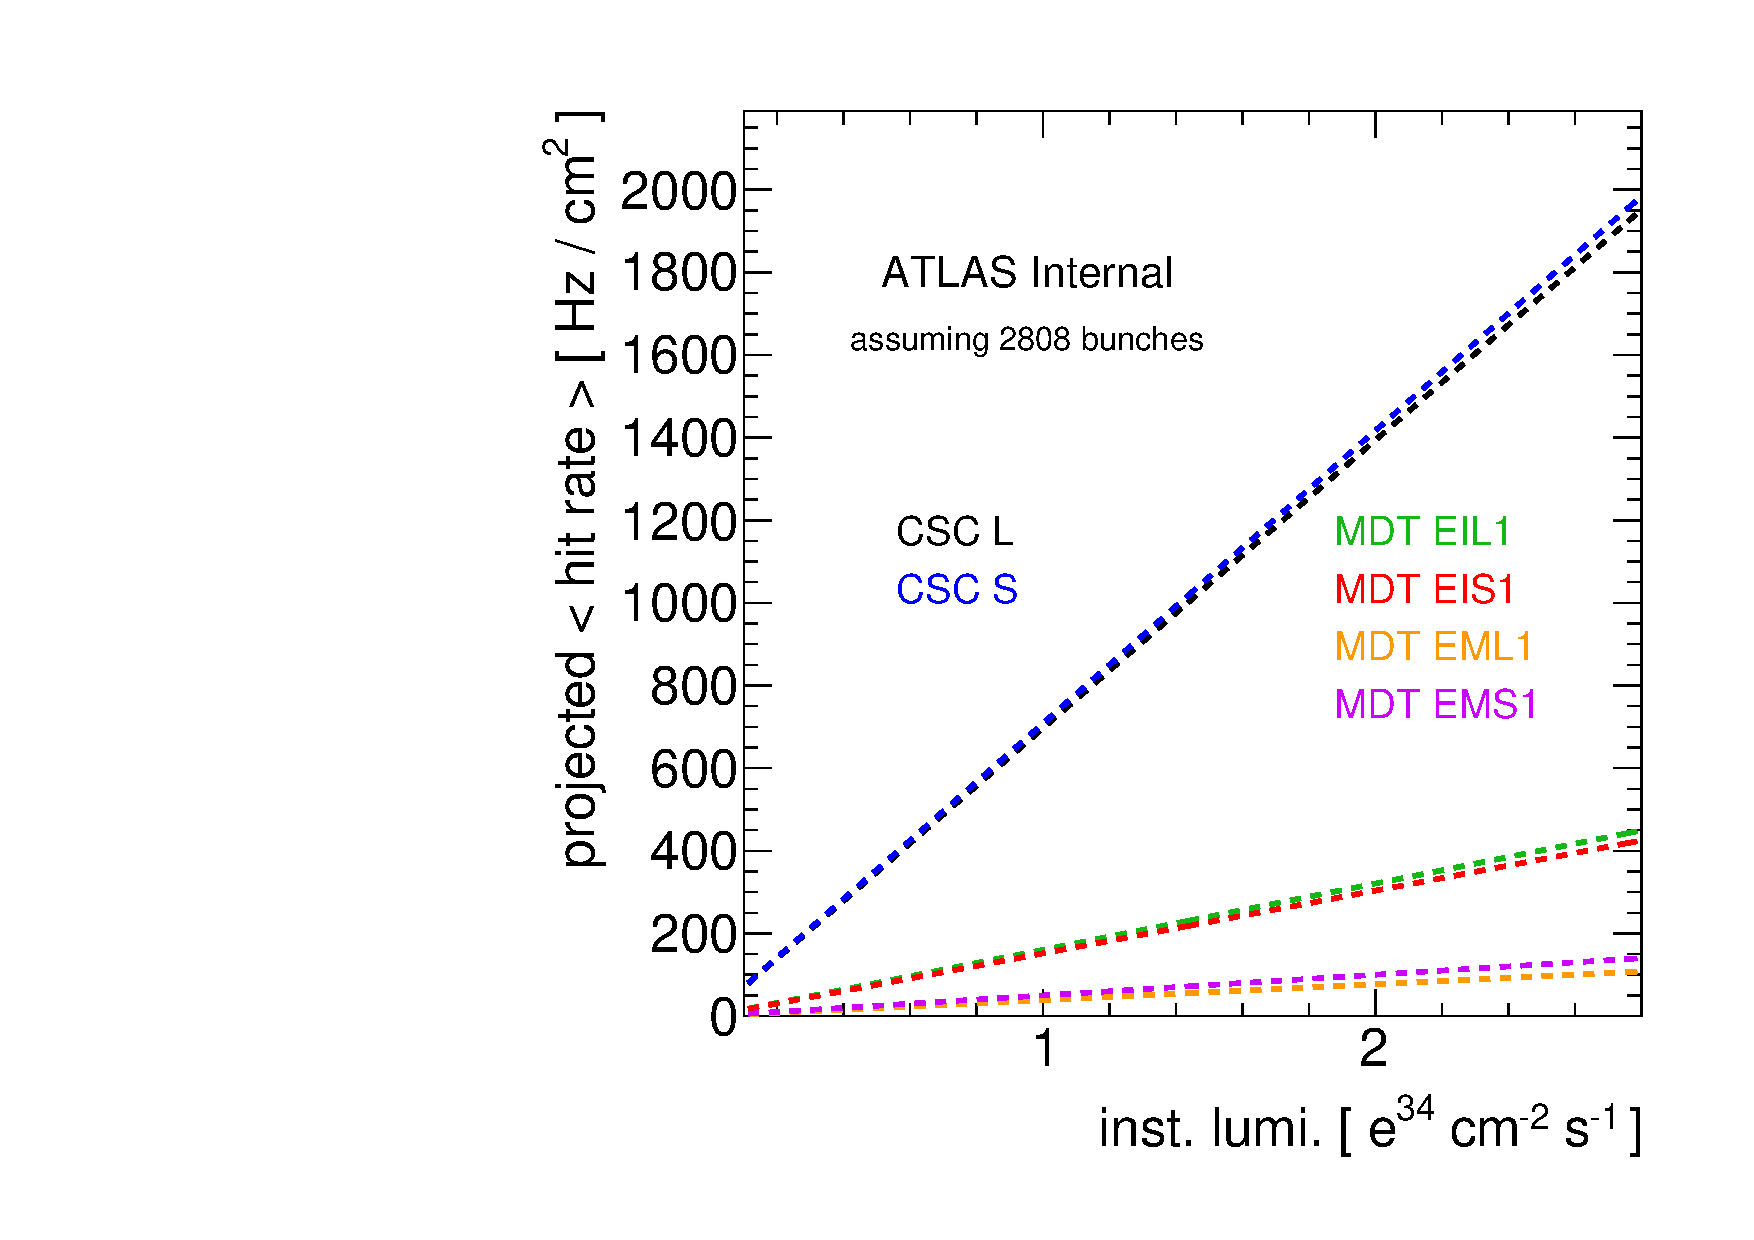
\includegraphics[width=0.45\textwidth]{./figures/extrapolate_vs_lumi_adc_2808.pdf}
    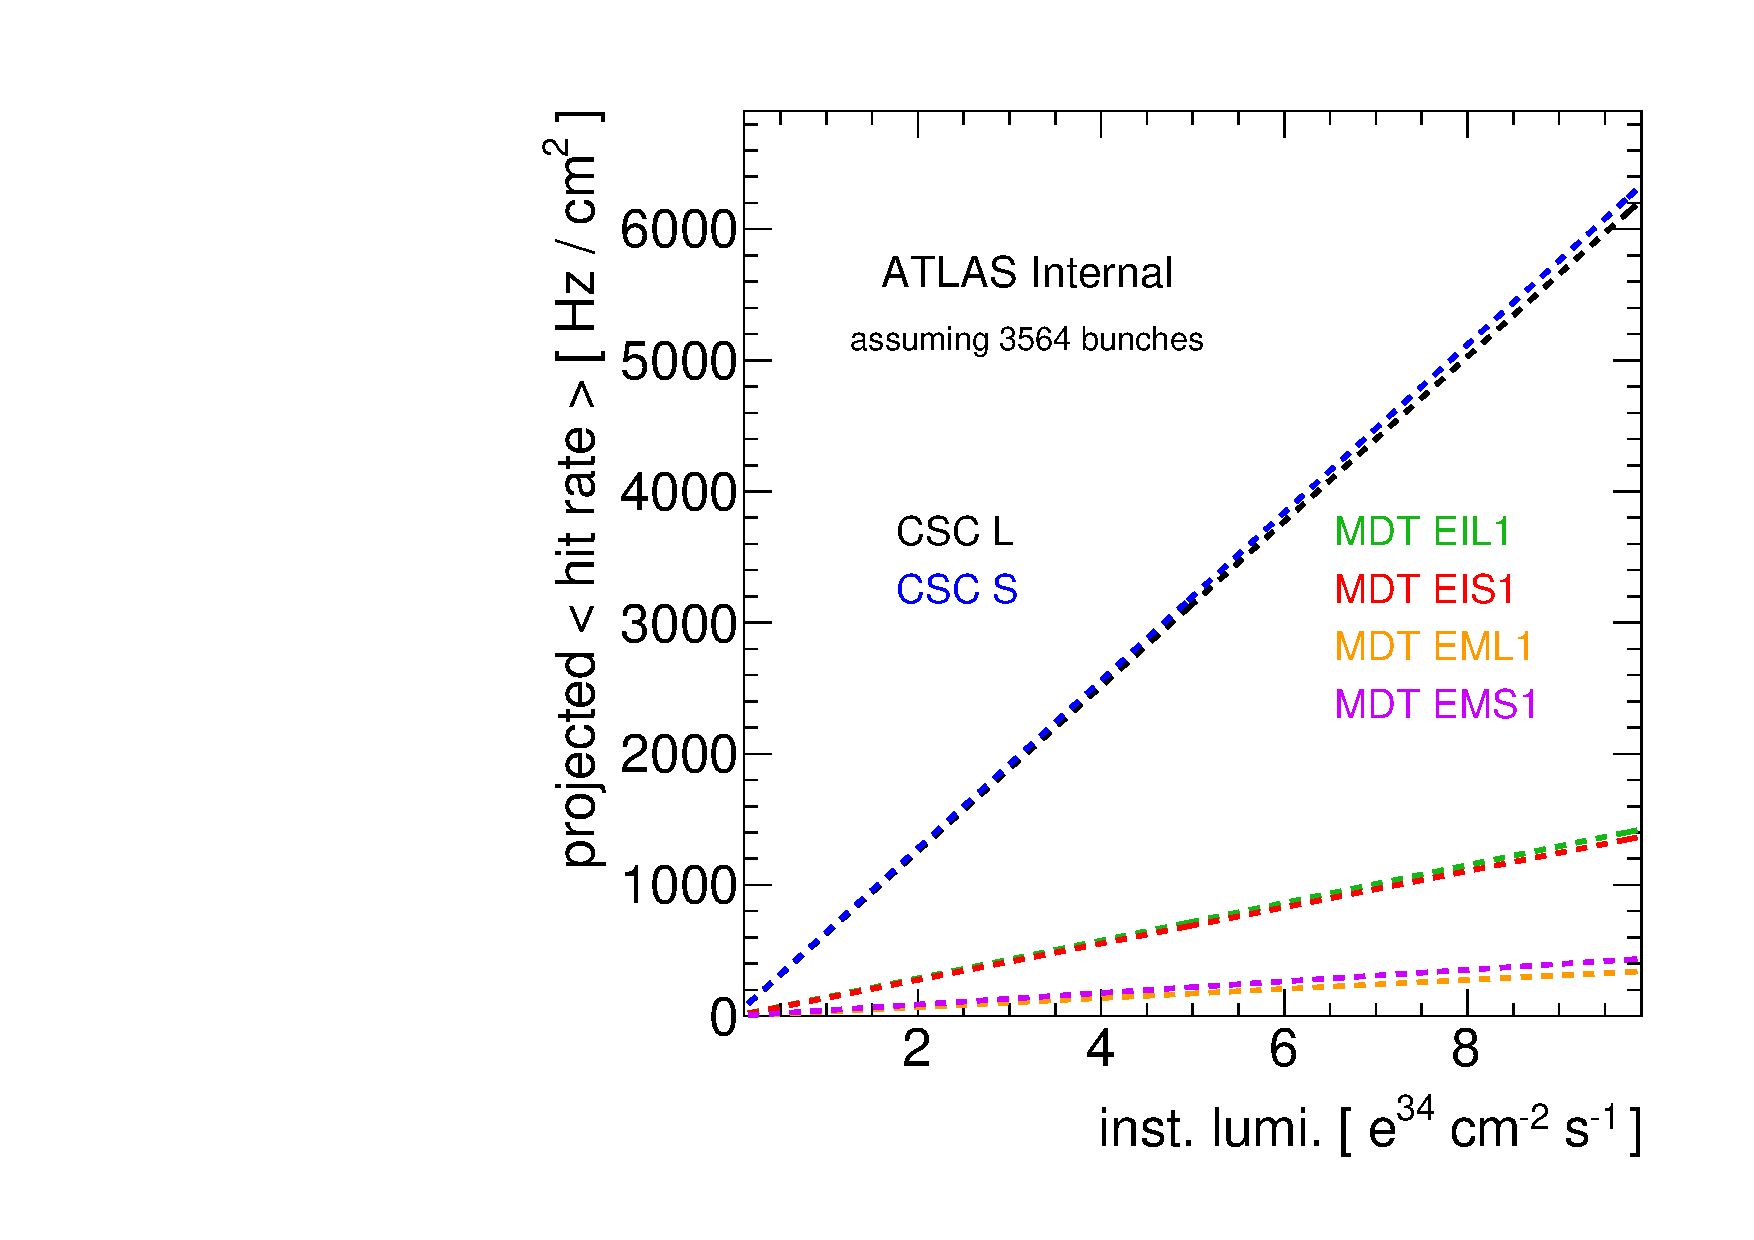
\includegraphics[width=0.45\textwidth]{./figures/extrapolate_vs_lumi_adc_3564.pdf}
    \caption{Projected average hit rates in the MS as a function of instantaneous luminosity, assuming 2808 (left) and 3564 (right) filled bunches in the LHC. The CSC and MDT EI regions are overlaid.}
    \label{fig:extrapolations-hitrates-adc}
  \end{center}
\end{figure}

% The CSC hit rate in 2015 data-taking closest to the beampipe is 1.94 (2.28) times larger than the average hit rate of the large (small) chambers. This implies the hottest region of the NSW will have a hit rate of between 8535 and 10214 $\text{Hz} / \text{cm}^2$, depending on the number of filled bunches in the LHC, and assuming no changes to the shielding of the MS or the beampipe. The projected hit rates with quality criteria requirements are 10-15\% lower than the inclusive projected hit rates.



\printbibliography

\end{document}
